\documentclass[a4paper, 12pt]{report}
\usepackage{indentfirst}
	\setlength{\parindent}{2.30em}
    \setcounter{tocdepth}{4}
    \setcounter{secnumdepth}{4}
	
\usepackage{pdflscape}
\usepackage{subfigure}
\usepackage{rotating}
\usepackage{wrapfig}
\usepackage{lscape}
\usepackage{booktabs,tabularx}
\usepackage{mathptmx}
\usepackage{amsmath,amssymb,amsfonts}
\usepackage{algorithm, algorithmic}
\usepackage{wasysym}
\usepackage{bm}
\usepackage{cleveref}
\usepackage{xfrac}
\usepackage{palatino, url}
\usepackage{minted}

\usepackage[top=4.572cm, bottom=3.175cm, left=3.81cm, right=3.175cm]{geometry}
\usepackage{sectsty}  % section font size
	\sectionfont{\normalsize}
	\subsectionfont{\normalsize}
	\subsubsectionfont{\normalsize}
	\paragraphfont{\normalsize}
	\subparagraphfont{\normalsize}

\usepackage{siunitx}
\usepackage{etoolbox} % remove spaces before and after paragraph
\usepackage{setspace} % control linespacing
	\setstretch{2}
%\usepackage{apacite}
%\usepackage{IEEEtrantools}
\usepackage{natbib}

\usepackage{graphicx}
	\graphicspath{{./Figures/}}
	\DeclareGraphicsExtensions{.pdf,.jpeg,.jpg,.png}

\usepackage{textcomp}
\usepackage[dvipsnames]{xcolor}

\usepackage{caption}
\captionsetup{format=hang, font=normalsize, labelfont=bf, justification=justified, labelsep=period}

% Pagination

\usepackage{fancyhdr}
	\pagestyle{fancyplain} % <- use fancyplain instead fancy
	\fancyhf{}
	\fancyhead[R]{\thepage}
	\renewcommand{\headrulewidth}{0pt}

\makeatletter
	\patchcmd{\@makechapterhead}{\vspace*{60\p@}}{}{}{}% Removes space above \chapter head
	\patchcmd{\@makeschapterhead}{\vspace*{50\p@}}{}{}{}% Removes space above \chapter* head
	\chapterfont{\normalsize \centering \MakeUppercase}

\begin{document}
\begin{titlepage}
	\setlength{\topmargin}{-40pt}
	\setlength{\textheight}{664pt}
	\addcontentsline{toc}{chapter}{\MakeUppercase{Title Page}\vspace{-0.5cm}}
	\begin{singlespace}
		\begin{center}
			\textbf{\MakeUppercase{Design and Development of 3D Point Cloud Scanner System (3D-PCSS) based on 2D LiDAR with A Web-based Application for Flour Product Storage Volume Measurement}}
			\vspace{2.50cm}

			\MakeUppercase{A THESIS}

			\vspace{2.0cm}

			Presented to the Faculty of\\
			Department of Computer Applications\\
			College of Computer Studies \\
			Mindanao State University -- Iligan Institute of Technology

			\vspace{2.0cm}


			In Partial Fulfillment\\
			of the Requirements for the Degree\\
			MASTER OF SCIENCE IN COMPUTER APPLICATIONS

			\vspace{2.25cm}

			\textbf{JAAFAR J. OMAR}

			\vspace{3.0cm}

			\textbf{ENGR. CARL JOHN O. SALAAN, Ph.D.} \\
			Adviser
			\vspace{2.0cm}

			March 2023

		\end{center}
	\end{singlespace}
\end{titlepage}

\pagenumbering{roman}
\tableofcontents
\listoffigures
\listoftables

\pagenumbering{arabic}

\renewcommand{\thechapter}{\Roman{chapter}}
\chapter{Introduction}
\renewcommand{\thechapter}{\arabic{chapter}}
\label{ch:Introduction}
\thispagestyle{empty}

\section{Background of the Study}
\label{intro:sec:Background of the Study}

Agricultural raw materials, such as rice, wheat, and corn, which mostly include solid, liquid or powered, provide significant amounts of carbohydrates for use in industry and human nutrition . Certain grains require little processing and can be eaten right away after harvest, while others must be prepared through a number of primary and secondary milling steps. As farmers learned to produced more resulting of various agricultural innovation, this raw materials must preserve the quality for future consumption \citep{Bucklin2019175}.
It is expected an increase in raw materials annually does necessitate an efficient post-harvest processes such as raw product storing method incorporating modern technologies \citep{Kumar2017-jl,yegorova_2021,Joni2022}.

Various tools and methods have been developed to measure stored raw materials volume inside an industrial storage silos or bins, employing sensors like contact level indicators (e.g., tilt switches, pressure diaphragms, rotary paddles) and non-contact indicators (e.g., stereovision, radar, ultrasound, lasers). Contact sensors offer cost-effective, dust-resistant point measurements but lack surface detail. Non-contact sensors can map grain surfaces accurately but require permanent mounting, are relatively expensive, and are susceptible to dust interference. However, conventional volumetric measurement method using weighted fiberglass tape is still being used providing only a single data point which leads to inaccuracy and error-prone volume measurement \citep{turner2016,turner2017}.

Point cloud data consists of a set of points representing an object in either a two or three-dimensional structure. This data typically comprises X, Y, and Z coordinates, but modern point clouds may also include additional information such as intensity, RGB values, and more \citep{wang2019306, stojanovic2023point}.

Light Detection and Ranging (LiDAR) is one of the many devices that can gather 3D points that often refer as point clouds. Unfortunately, commercial 3D LiDAR systems tend to be expensive in comparison to their 2D-based LiDAR. This cost disparity can lead to limitations in accessibility for certain applications or industries, hindering widespread adoption and innovation in fields where 3D spatial data is crucial. Low-cost two axes-based LiDAR can mimic the collection of 3D point cloud by adding an additional axes using tilting device \citep{clar2022}. However, it comes with a notable drawback: it lacks several capabilities present in high-end 3D LiDAR systems, including multi-echo functionality, long-range detection, high angular resolution, among others.

Recent innovations in various industries have made the production less manual but producing more by using automation and wireless technologies that helped to produce better and accurate measurement compared to traditional methods. These approaches include various sensing technologies, automated measurements, machine to machine (M2M) communications, and monitoring systems. The interconnected sensors and actuators allow to remotely collect data, store, and process the data to provide better insight in the industry and also for the economic growth, specify the characteristics of a paperless factory, it is a development of a smart factory in which all data that is turned into information is stored, transferred, and displayed entirely remotely and digitally. As the level of digitization of a smart factory, it is not a revolution but rather an evolution \citep{bulut2020}.

%Although laser  technology have been proved to be useful and excellent in various field compared to other technology with in terms of its capabilities, features, and accuracy, however, it produced undesirable or no data when the environment is exposed to dust or fog the blocks the visibility of the object interest \citep{yigit2015,turner2017,duysak2020}. With the given circumstances, todays commercial high-end LiDAR still gather relevant data to analyze using multi-echo functionality and some hardware improvement which, unfortunately, lacks on low-cost LiDAR.

\section{Statement of the Problem}
\label{intro:sec:Statement of the Problem}
%A variety of product that stored in a silo can be solid, powdered and liquid. When the product such as solid grains, corn are being stored, minimal dust cloud are generated during filling process. However, when powdered products such as cement or flour are being filled, a dense dust cloud are created. Ideally, when LiDAR is used for measuring the distance between the product and the door, it is installed at the top. Due to the fine-texture of solid materials such as flour product, a dispersed dust cloud may form during the pneumatic conveying process of loading flour into the bin \citep{williams2007}. Although LiDAR sensor have the ability to provide faster data collection and detailed spatial illustration compared to other sensing technologies, and the precision of distance measurement is undeniable, the wavelengths that LiDAR operates, typically, 700 to 900 nm can be problematic when deposit layers of dust formed caused by stored product as it may caused a problem when scanning the spatial structure of the product.

While some food manufacturing industries still rely on manual and labor-intensive storage measurement procedures, there is a growing need to adopt advanced technologies with remote capabilities. This shift aims to eliminate the need for frequent physical processes that may endanger employees. Additionally, monitoring the volume of raw product storage, particularly in industries dealing with essential commodities like flour, holds paramount importance for various reasons. Ensuring accurate and timely monitoring of storage bins prevents detrimental scenarios such as underproduction or overstocking. In the case of underproduction, inadequate monitoring leading to stockouts can disrupt the production process, resulting in delayed deliveries and potential loss of sales. Conversely, overstocking can lead to unnecessary inventory costs, space constraints, and increased risk of product spoilage or infestation. Specifically, in the context of flour storage, overstocking can attract flour beetles, leading to infestation and contamination of the stored flour when left unsold. Thus, precise volume monitoring is crucial to maintaining optimal inventory levels, facilitating efficient production planning, and mitigating the risk of financial losses and product quality issues for food manufacturing industries.

%Silo storage systems are versatile, accommodating a wide range of products, including solids, powders, and liquids. One characteristic of product storages is that when they are filled with raw materials, except for liquids, they create a dust cloud in the empty space. Solid grains like corn typically produce minimal dust clouds during filling, whereas powdered substances like cement or flour often generate dense dust clouds.

%When implementing LiDAR for storage volume measurement, the ideal placement is at the top of the silo. However, in the case of fine-textured solid materials such as flour, dispersed dust clouds may arise during the pneumatic conveying process of loading flour into the bin \citep{williams2007}. Although LiDAR sensors offer advantages such as rapid data collection and precise spatial representation compared to alternative sensing technologies, their operational wavelengths—usually between 700 to 900 nm—can pose challenges when scanning through layers of dust deposited by stored products. This challenge may potentially impact the accuracy of spatial structure scans.

This study presents the development of a volumetric measurement system for raw materials storage bin. The system is designed to be controlled and scanned remotely using a web-based interface, alleviating the manual process of volume measurement. Additionally, this study investigates the behavior of the system when dust clouds are present during filling due to fine texture of some raw materials such as flour.

%There are various advanced LiDAR technologies such as 3D LiDAR sensors that are available in the market, primarily used for robotics applications, that can address these problems without the need of additional hardware and software configuration. However such sensing devices are too expensive and sophisticated. The focus of this study is to utilized low-cost LiDAR technology to partially mimic the sophisticated functionality of the above mentioned technology.

\section{Objectives of the Study}
\label{intro:sec:Objectives of the Study}
The general objective of this study was to develop a system that can remotely measure the volume of the product inside of a flour storage bin using point cloud data and web-based Application. The following specific goals were completed:

\begin{enumerate}
	\item Designed and developed a 3D point cloud scanner system (3D-PCSS);
	\item Developed a web-based application for remote access to 3D-PCSS system and visualization for point cloud and volume measurement;
	\item Tested and evaluated the performance of the system.
\end{enumerate}

\section{Originality of the Study}
\label{intro:sec:Originality of the Study}
The originality of this study lies in the development of a system capable of remotely estimating and monitoring the volume and capacity of storage materials. This study introduces two distinct components: the point cloud acquisition system and the web application system designed for remote monitoring purposes. Furthermore, the study explores the system's behavior in the presence of dust, providing insights for further enhancement and modification.

\section{Scope and Limitations}
\label{intro:sec:Scope and Limitations}
The scope of this study is to develop a volume estimation system through remote point cloud acquisition and a web application. It is important to note that the system testing was not conducted directly in a commercial manufacturing industry or an actual industrial storage bin. Instead, testing took place in an open area using a mock-up storage bin designed to replicate the size and shape of a typical industrial storage facility. Additionally, the study exclusively focuses on utilizing flour as the primary raw material for testing purposes.


\section{Significance of the Study}
\label{intro:sec:Significance of the Study}

Accurate and efficient post-harvest processes are vital in the food industry to ensure effective inventory management and maintain an adequate supply of materials. Automation with remote sensing devices is a modern technology that can be integrated into a variety of industries, eliminating labor-intensive tasks that may expose employees to dangerous scenarios. The development of the 3D point cloud scanner system (3D-PCSS) addresses the need for precise volume measurement of stored flour within silo storage bins. By employing point cloud data and a web-based application, the system offers remote accessibility and visualization capabilities, allowing for convenient monitoring and management of storage facilities. This technological advancement, with potential integration into industrial settings, not only enhances efficiency in inventory management but also minimizes the risks associated with manual measurement procedures. Furthermore, the testing and evaluation of the system provide valuable insights into its performance and potential for further refinement, paving the way for future advancements in automated storage volume measurement systems.

\section{Conceptual Framework}
\label{intro:sec:Conceptual Framework}

\begin{figure}[H]
	\centering
	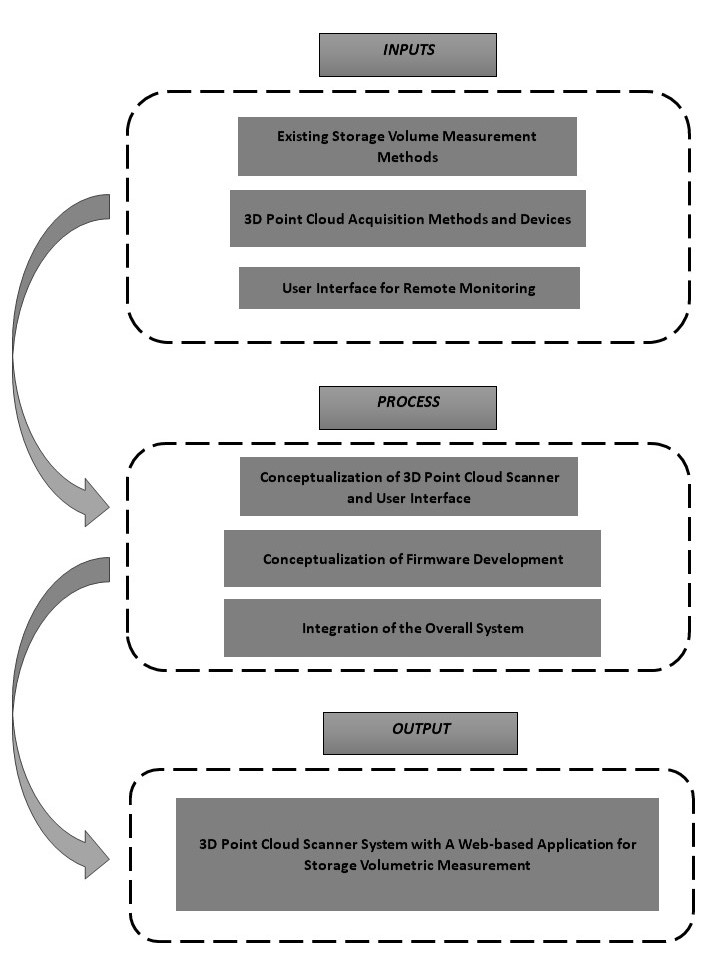
\includegraphics[width=1\textwidth, height=0.9\textheight]{concept_framework.jpg}
	\caption{General Conceptual Flow}
	\label{fig:conceptual-framework}
\end{figure}

Figure \ref{intro:sec:Conceptual Framework} outlines the conceptualization of the study. As shown in the figure, The conceptualization of the study are derived from the examination of prior studies and established methodologies. The study examined existing storage volume measurement methods, 3D point cloud acquisition methods and devices, and different user interface for remote monitoring. The output of this paper is the design and development 3D point cloud scanner system with a web-based application for Storage volumetric measurement. The general and specific objectives are presented in the previous section (see section \ref{intro:sec:Objectives of the Study}).

\section{Theoretical Framework}
\label{intro:sec:Theoretical Framework}
This section introduces the fundamental theories that guides the underlying principles, methodologies and technologies involved in the study.

\subsection{Calculating Storage Materials Volume using Depth Measurement}
The volume of stored grain is typically calculated using the depth measurement. Once the equivalent level height of the grain is determined based on the depth measurement and surface profile assessment, this height is multiplied by the conversion factor to obtain the volume of the stored grain. This calculation accounts for the headspace between the eave and the grain surface. The underlying calculation with a single and non complex geometric shape can be presented as follows:

\begin{equation}
	V = A \times h
\end{equation}

Where:
\begin{align*}
	V & : \text{Volume of the storage container}   \\
	A & : \text{Area of the base of the container} \\
	h & : \text{Height or depth of the container}
\end{align*}

\subsection{3D Polar Coordinate to Cartesian Coordinate}
Converting polar coordinates to cartesian coordinates in three dimensions involves considering the radial distance ($\rho$), the polar angle ($\theta$), and the azimuthal angle ($\phi$). Given a point in spherical coordinates ($\rho$, $\theta$, $\phi$), the corresponding Cartesian coordinates ($x$, $y$, $z$) can be calculated as follows:
\begin{equation}
	x = \rho \times \sin(\theta) \times \cos(\phi)
\end{equation}
\begin{equation}
	y = \rho \times \sin(\theta) \times \sin(\phi)
\end{equation}
\begin{equation}
	z = \rho \times \cos(\theta)
\end{equation}

Where:
$x$, $y$, and $z$ represent the Cartesian coordinates of the point.
$\rho$ is the radial distance from the origin to the point.
$\theta$ is the polar angle measured from the positive $z$-axis to the point.
$\phi$ is the azimuthal angle measured from the positive $x$-axis to the projection of the point onto the $xy$-plane.

\subsection{Point Cloud Data}
A set of points in three dimensions that represent an object's or scene's surface is called a point cloud. Point clouds can be generated through a variety of methods, including photogrammetry, LiDAR, and 3D scanning. Processing and evaluation of these point clouds for a variety of applications is an increasing area of point cloud processing.


\subsection{Computational Geometry using Convex Hull}
The study of the development and evaluation of algorithms for geometric problems in low dimensions—usually two or three—is known as computational geometry. As the smallest convex polygon containing a given set of points, the Convex Hull is a fundamental concept in computational geometry. The convex hull represents the smallest convex set enclosing a given set of points in a Euclidean space as figure \ref{ch1:fig:convex_hull_theory} illustrated. It adheres to principles of convexity, ensuring that the shape remains convex, and minimality, guaranteeing it encompasses the points with minimal expansion.

The Gift Wrapping algorithm, which has a time complexity of O(nh), where n is the number of points and h is the number of points on the hull, is one straightforward method for calculating the Convex Hull \citep{barber1996quickhull,chan1996optimal}.

The equation \ref{ch1:eq:convex_hull} defines the convex hull of a set of points $P_j$ in N-dimensional space. The variable $C$ represents a point in the convex hull, $\lambda_j$ are non-negative weights, and $A_j$ are some constraints. The summation iterates over all points from $j=1$ to $N$.

\begin{equation}
	\label{ch1:eq:convex_hull}
	C = \left\{ \sum_{j=1}^{N} \lambda_j P_j: \lambda_j \geq 0 \text{ for all } j \text{ and } \sum_{j=1}^{N} \lambda_j = 1 \right\}
\end{equation}




\begin{figure}[H]
	\centering
	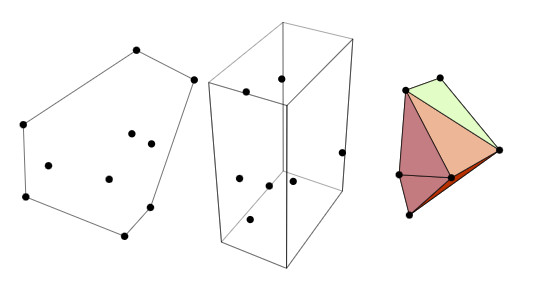
\includegraphics[width=0.8\textwidth]{convex_hull_3d}
	\caption{Convex Hull of Set of Points}
	\label{ch1:fig:convex_hull_theory}
\end{figure}

TODO: Add Polygon Mesh

\subsection{ROS Nodes, Topics, and Subscribe-Publish Relationship}
A framework for building complicated robotic systems that is adaptable is called Robot Operating System (ROS). It makes it possible for nodes, software components that carry out particular functions, to communicate with one another. Topics, also referred to as buses, are the methods by which nodes exchange messages with one another. A key component of ROS is the publish-subscribe connection, in which nodes can publish or subscribe to topics.

Nodes in ROS have the ability to simultaneously subscribe to an indefinite number of topics and share data to an indefinite number of topics. One of the main methods of data communication between nodes, and consequently between other components of the system, is through topics \citep{St-Onge2022}. A node must first advertise a topic before publishing content, or messages, into it in order to exchange information. The first part is completed in the node's initialization code, and the second is completed each time new data has to be shared, usually at a predetermined frequency inside the main loop of the code. Conversely, the node or nodes that need the content of a topic will subscribe to it. The subscriber will associate a callback function triggered for each new incoming message \citep{St-Onge2022}.

%These formulas allow you to convert spherical coordinates to Cartesian coordinates, providing a way to represent points in three-dimensional space using different coordinate systems.


%The research is based on the idea of using automation for industrial operations, specifically in the food industry. Point cloud data is a collection of an unorganized set of x, y, and z coordinates in a three-dimensional space. There are various ways to acquire point cloud data, and one possible way is through active non-contact sensing technology such as LiDAR sensor. LiDAR uses Time-of-Flight (TOF) method of measuring distance between the sensor to the object. TOF scanners are inexpensive compared to other specialized 3D scanners \citep{chua2017}. The researcher will utilize LiDAR to acquire 3D point cloud data because of its ability to gather points data and converts them into a global world coordinate frame \citep{bi2021}. The study does, however, acknowledge the potential limits of LiDAR, when the environment is prone to medium (e.g., water vapor, gases, dust particle, etc.) that can obstruct the target surface, the LiDAR acquired point cloud data that may alter the precision of the data \citep{chua2017}. Thus, the researcher will manage the raw point cloud data by filtering the factoring medium such as dust. Lastly, Delaunay Triangulation is a computational geometry computation that connects a set points to form a mesh of triangles. It can be used for volume estimation by calculating the volume of a convex hull which will be use in this study.

\section{Definition of Terms}
\label{intro:sec:Definition of Terms}

\begin{enumerate}
	\item \textbf{LiDAR} \textemdash stands for Light Detection and Ranging, can also be describe as Light Imaging, Detection, and Ranging. It is a method for determining ranges by targeting an object or a surface with a laser and measuring the time-of-flight to determine the distance.

	\item \textbf{Bin} \textemdash is a large container used to store materials, such as grain, coal, sand, or other bulk goods. They are typically made of metal, plastic, or wood and come in various sizes, shapes, and designs.

	\item \textbf{ROS} \textemdash Robot Operating System is a set of open-source libraries and tools designed to help developers build robot applications. It provides a common framework for creating, managing and sharing code, data, and other resources related to robotic systems.

	\item \textbf{Point Cloud} \textemdash is a set of data points in a three-dimensional space, typically representing the surface of an object. Each point in the cloud is defined by its three-dimensional coordinates (x, y, and z) and may also include additional information such as color, intensity, or normal vector.
	\item \textbf{Convex Hull} \textemdash is the minimum convex polygon from the set of points that encompasses all of the points in the set.

\end{enumerate}
\renewcommand{\thechapter}{\Roman{chapter}}
\chapter{Review of Related Literature}
\renewcommand{\thechapter}{\arabic{chapter}}
\label{ch:rrl}
\thispagestyle{empty}

Enhancing post-harvest processing and storage technology is essential meeting increasing global demand and minimizing waste. Improved technology ensures efficient supply chains and reduces losses due to spoilage, damage, or inefficient methods. Moreover, advanced monitoring and management techniques not only enhance production but also contribute to safety standards \citep{Kumar2017-jl,Joni2022}.

In this chapter, various relate topic were reviewed and discussed. Different methods, technologies and implementation were also introduced and examined.

\section{Overview of Existing Methods, Techniques and Technologies Used for Volume Measurement}

%In this chapter, the researcher discussed the general idea of the volume estimation and filtering method and its several related studies. The chapter also presented some published and unpublished methods and technologies used for measuring the level and volume of the materials inside the silo (or sometimes called bin).
According to \citet{turner2016}, the determination of grain volume in a bin depends on variables like bin diameter and corresponding level height of grain. Different surface condition assessment, however, is subjective and subject to a number of variables, such as operator experience, visibility, lighting, and ambient circumstances. Various strategies can be used to improve volume estimate; standard angles of repose for various grain types are provided in the literature.

Traditional level measurements are already used and studied in different industries such as weight and cable methods, ultrasonic, Guided Ware Radar (GWR), and Thru-air Radar (TAR) which has their own advantage and disadvantages. Ultrasonic and laser technologies are excellent in providing accurate and detailed measurement of level. However, these technologies are problematic when in terms of dusty environment \citep{duysak2020}. Additionally, Various tools and methods have been developed to measure stored raw materials volume inside an industrial storage silos or bins, employing sensors like contact level indicators (e.g., tilt switches, pressure diaphragms, rotary paddles) and non-contact indicators (e.g., stereovision, radar, ultrasound, lasers). Contact sensors offer cost-effective, dust-resistant point measurements but lack surface detail. Non-contact sensors can map grain surfaces accurately but require permanent mounting, are relatively expensive, and are susceptible to dust interference. However, conventional volumetric measurement method using weighted fiberglass tape is still being used providing only a single data point which leads to inaccuracy and error-prone volume measurement due to uneven materials  surface topology \citep{turner2016,turner2017}.

New methods and technologies have been trying to incorporate in industrial settings to enhance the measurement methods such as using Microwaves Radar \citep{vogt2017}, Horn Antennas-based \citep{duysak2020, yigit2015}, Load Cell, Ultrasonic, Laser-based \citep{geuvara2020}, and Temperature-based sensor \citep{rhee2021}.

\section{Point Cloud Acquisition Devices}
\label{rrl:sec:3D Point Cloud acquisition}
The recent advancements in spatial acquisition technologies such as 3D laser scanning, photogrammetry, videogrammetry, RGB-D camera, and stereo camera have resulted in the formation of point clouds that may contain millions, billions, or trillions of points \citep{jaboyedoff2012}. Various 3-dimensional scanning technology produces data that are formatted as point cloud, typically these point cloud data acquired using laser or image scanner. These gathered data can be managed to ease the measurement and visualization of an object or environment \citep{chua2017}. Point cloud data are processed to generate desired output on the specific application. Over the past 20 years, the advent of high-quality 3D point cloud acquisition changes the perspective of robotics. Moreover, 3D scanning through various technologies enable the possibility of less contact for physical measurement that eliminate the traditional approach that involves time and effort. These technologies vary in size, functionality, and cost, ranging from affordable options to more complex and expensive ones \citep{rusu2011}.


\subsection{Light Detection and Ranging (LiDAR)}
\label{rrl:subsec:Light Detection and Ranging}
LiDAR, a remote sensing technology, employs laser light to create precise 2D or 3D models of objects or environments. Apart from Time-of-Flight (ToF) and triangulation, which measures distances based on the angle and timing of laser pulses, LiDAR systems utilize other techniques such as amplitude modulation and frequency modulation. These techniques vary in how they measure distances and capture data. By integrating data from multiple laser pulses, LiDAR generates a comprehensive point cloud that accurately represents the shape and structure of the objects within the environment, Figure \ref{fig:Typical LiDAR System} shows the block diagram of a typical LiDAR system. LiDAR technology have been used in industrial settings. In the context of LiDAR scanning, individual point cloud scans are acquired and processed for a specific area. These point clouds are then merged and blended together to generate a complete point cloud of the desired area, which can be utilized for distance and measurement calculations \citep{jaboyedoff2012, raj2020}.

\begin{figure}[H]
	\centering
	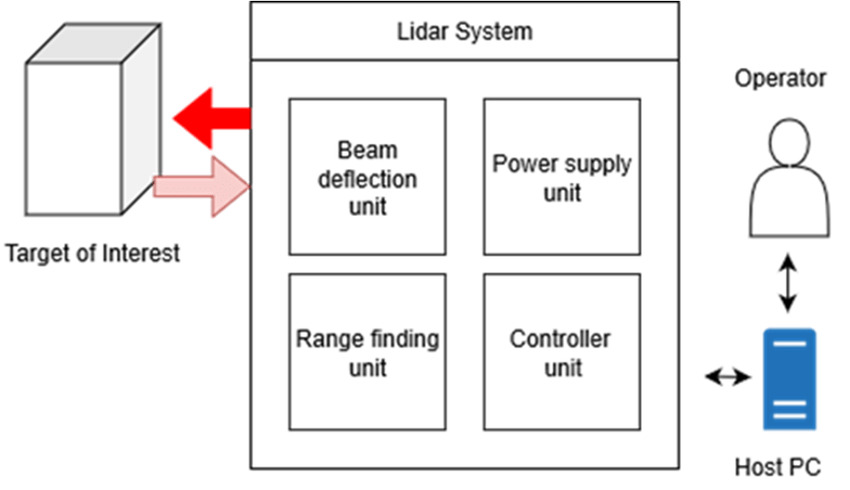
\includegraphics[width=0.9\textwidth]{Figures/Block-diagram-of-light-detection-and-ranging-LiDAR-system} % second figure itself
	\caption{Typical LiDAR System}
	\label{fig:Typical LiDAR System}
\end{figure}

A 360-degree scan of a LiDAR is generally obtained as shown in figure \ref{fig:360-dgree-lidar-scan} to produce a 2D map, a typical scan using the robot's top-mounted 2D LIDAR. The axis of the rotating LIDAR sensor is shown as a red line. The border of the surrounding obstacles is indicated in blue \citep{sarker2020}.

\begin{figure}[H]
	\centering
	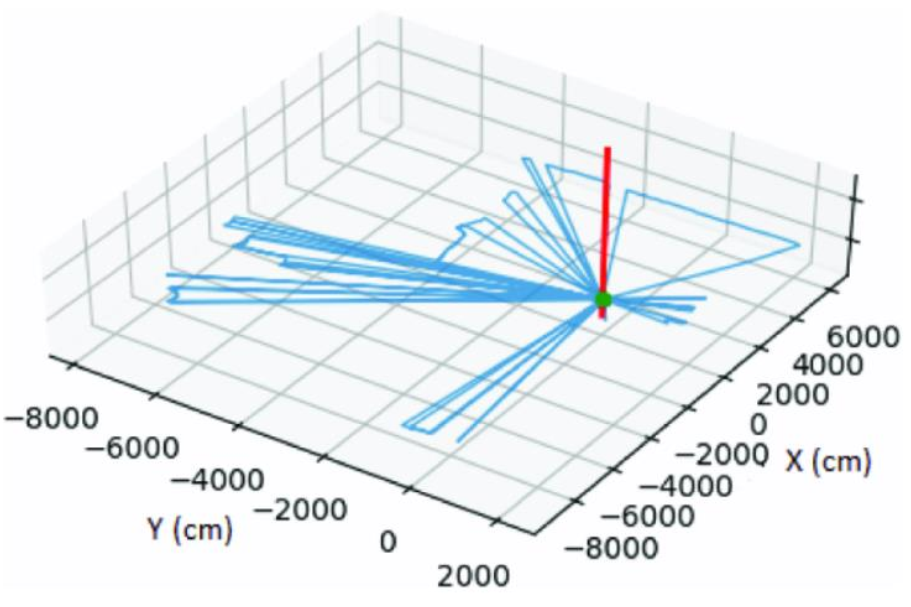
\includegraphics[width=0.9\textwidth]{Figures/360-degree-lidar-scan.png} % first figure itself
	\caption{360-degree scan of 2D LiDAR}
	\label{fig:360-dgree-lidar-scan}
\end{figure}

\subsection{Rotating 2D LiDAR Scanner into a 3D Point Cloud Scanner: Mechanisms and Techniques}
A 2D LiDAR scanner, typically used for horizontal plane scanning, can be transformed into a 3D point cloud scanner with the addition of extra components and processing techniques. One common method involves incorporating a rotating mechanism, such as a pan-tilt unit (PTU), to the 2D LiDAR. As the LiDAR rotates, it collects data points at various angles, generating a series of 2D scans. These scans are then combined and processed using algorithms to reconstruct a 3D representation of the surroundings. Integrating the 2D LiDAR device with electric motors into various configurations enables the acquisition of 3D scans. Figure \ref{fig:four_different_configurations} illustrates four such configurations: pitching, rolling, yawing, and top yawing scans \citep{raj2020}.

\begin{figure}[H]
	\centering
	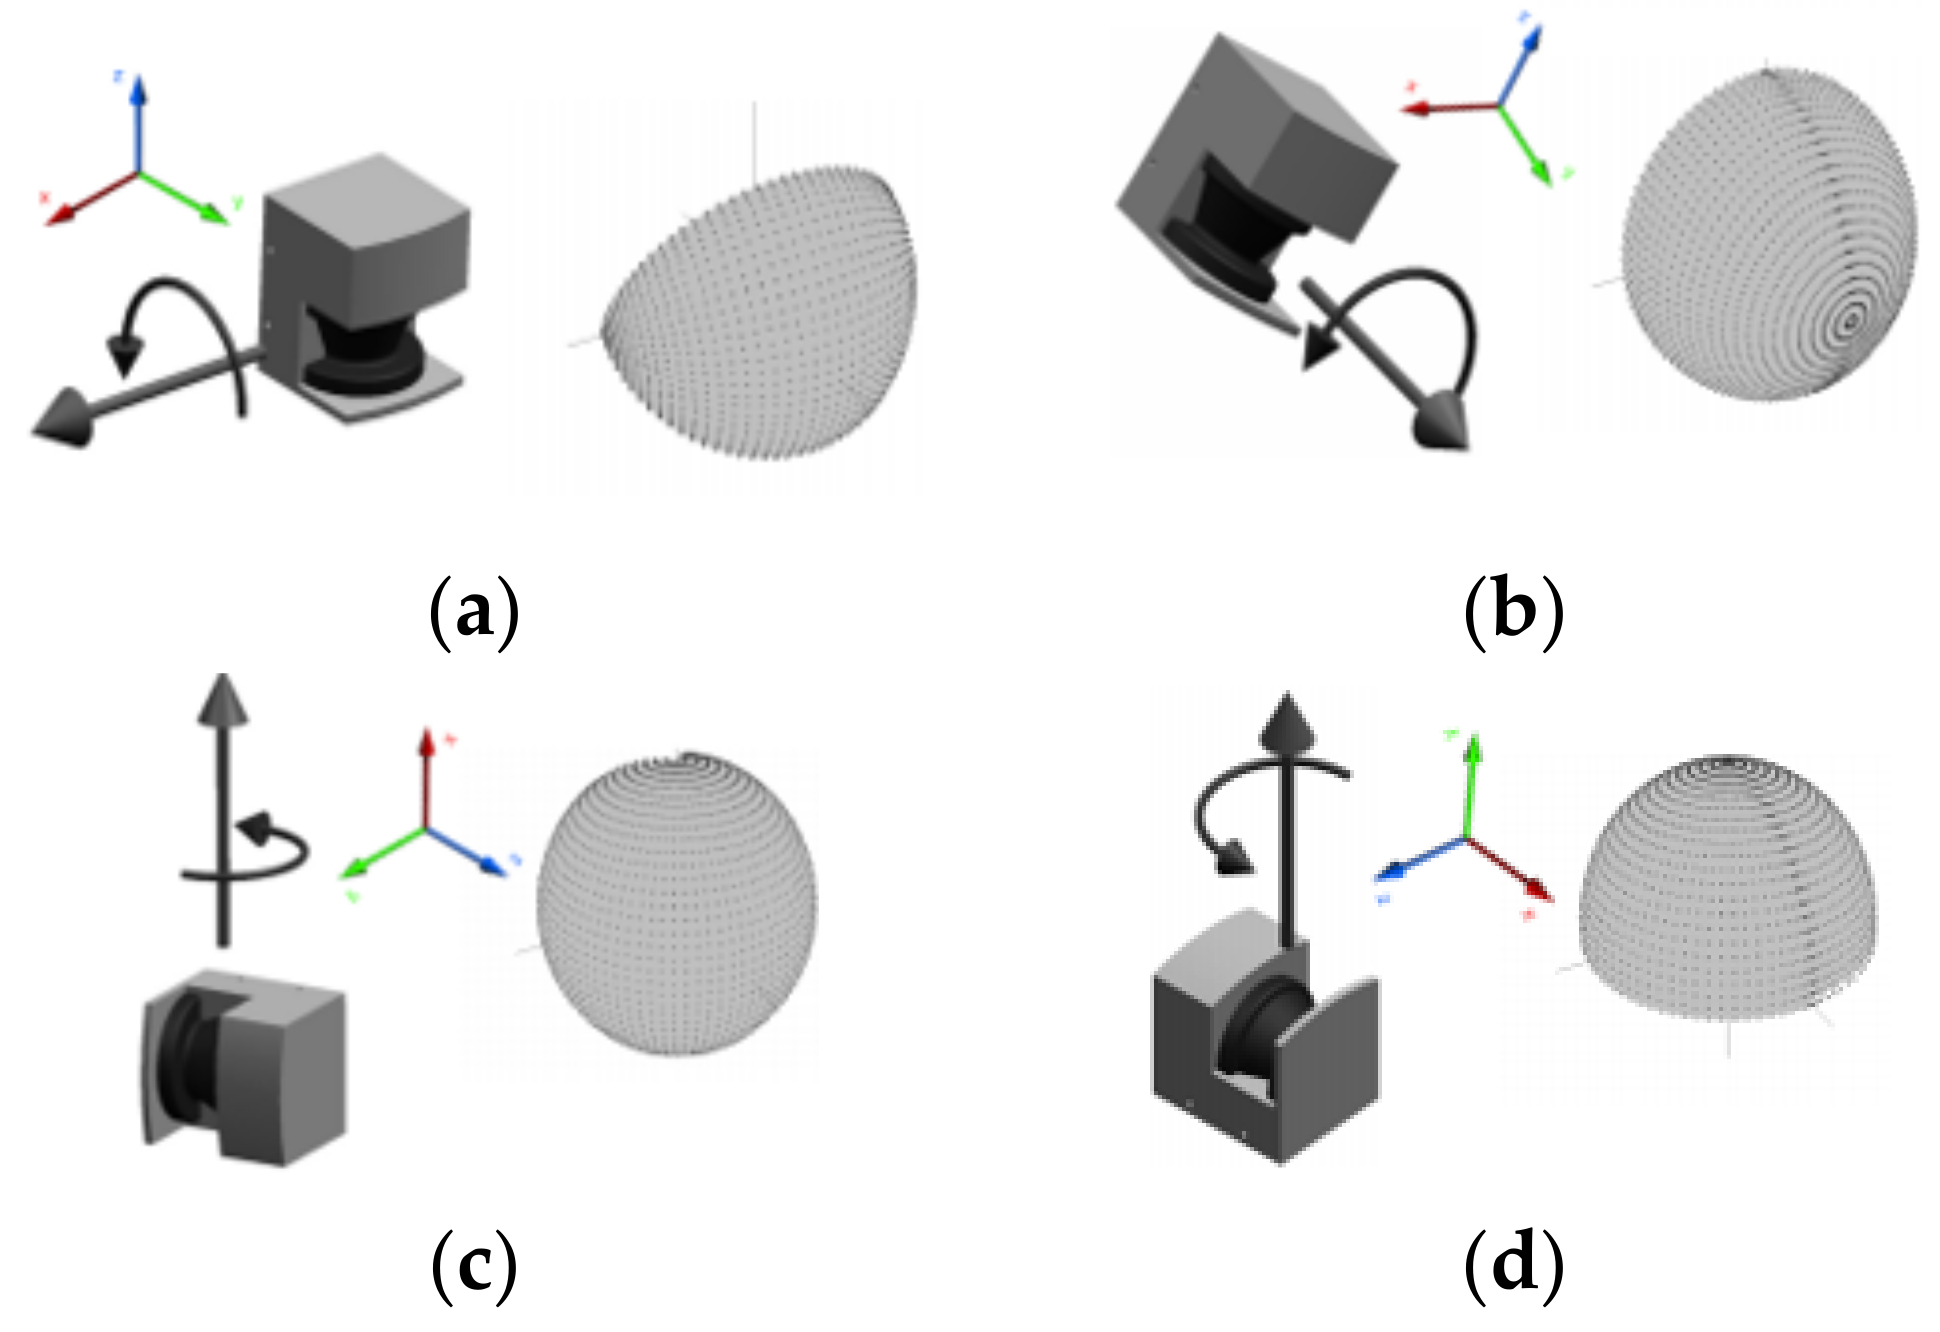
\includegraphics[width=0.9\textwidth]{Figures/tilting} % include your image file here
	\caption{Four different configurations for rotating: (a) pitching scan, (b) rolling scan, (c) yawing scan, (d) top yawing scan}
	\label{fig:four_different_configurations}
	\medskip
	\normalsize Source: \citep{raj2020}
\end{figure}

% \begin{figure}[H]
% 	\centering
% 	\begin{minipage}{0.5\textwidth}
% 		\centering
% 		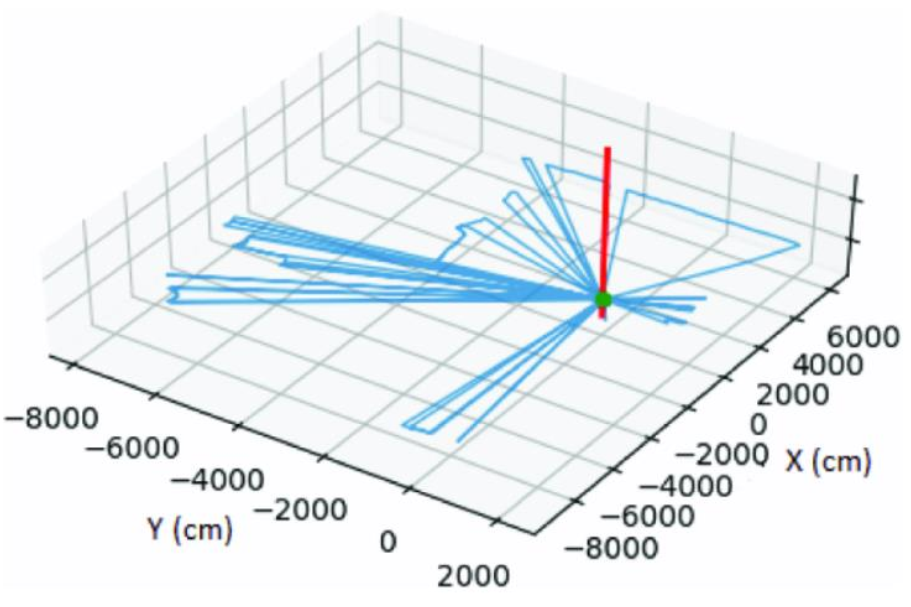
\includegraphics[width=0.9\textwidth]{Figures/360-degree-lidar-scan.png} % first figure itself
% 		\caption{360-degree scan of 2D LiDAR}
% 		\label{fig:360-dgree-lidar-scan}
% 	\end{minipage}\hfill
% 	\begin{minipage}{0.5\textwidth}
% 		\centering
% 		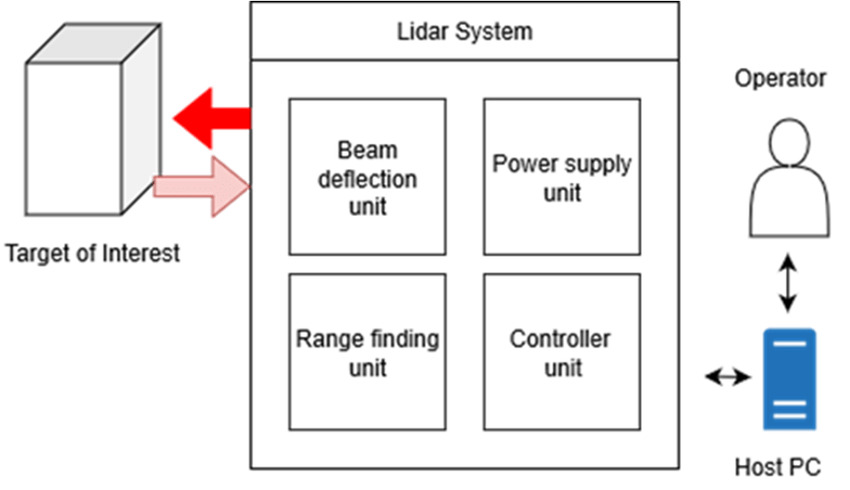
\includegraphics[width=0.9\textwidth]{Figures/Block-diagram-of-light-detection-and-ranging-LiDAR-system} % second figure itself
% 		\caption{Typical LiDAR System}
% 		\label{fig:Typical LiDAR System}
% 	\end{minipage}
% \end{figure}

\citet{kang2018} utilized a 2D low-cost off-the-shelf LiDAR to reconstruct complex 3D model by integrating an external rotary for additional dimension. The experimental test achieved to evaluate 3D reconstruction by concluding that using a low-cost 2D LiDAR sensors can  perform 3D point cloud acquisition but increase either the complexity of its hardware or software.

A stepper motor was used in the study conducted by \citet{yuan2021} and \citet{kang2018} to rotate a 2D LiDAR. However, in the study conducted by \citet{yuan2021}, the rotating 2D LiDAR with initial motor shaft position defined using a combination of photoelectric switches and shading sheets, to create a 3D point cloud representation of the environment. The main objective of the study was to minimize the cost by utilizing stepper motor. Intensive calibration was conducted to correct the error of the system due to lack of the absolute angle position of the motor, thus, the study focus on calibrating the system by synchronizing the 2D LiDAR with the stepper motor.

In a previous study by \citet{clar2022}, a servo motor was employed to rotate a 2D LiDAR, with calibration performed to synchronize the LiDAR's movement. However, the system in that study relied on a laptop and microcontroller for operation. While adequate for experimental testing, this setup posed challenges for larger-scale deployment due to its size, weight, and power demands. Consequently, there arose a need for a more compact and portable solution to address these limitations.

The primary problem with calibration and synchronization between a 2D lidar and a servo arises from the lack of an absolute angle reference for the servo. Unlike encoders or sensors that provide precise angular measurements, servos typically lack absolute positioning capabilities. Although rotating 2D LiDAR can never replace commercial 3D LiDAR with several reasons, however, rotating 2D LiDAR can be partially used and installed with in terms of static and nonmoving environment \citep{bi2021}.

TODO: ADD AUTHORS THAT USES ADDITIONAL functionality FOR 2D TO 3D

\section{Volume Measurement Using 3D Point Cloud Data}

Utilizing the latest advances in volume measurement with 3D point cloud data is an innovative method that precisely determines the volume of spaces or objects in a three-dimensional environment. This technique makes precise and thorough volumetric analysis possible by using point cloud data, which frequently consists of millions of points in 3D space. The concepts, procedures, and uses of volume measurement with 3D point cloud data will be covered in explain in this section, along with examples of its relevance in various domains \citep{zhi2016,meng2023}.

\subsection{Frameworks for Point Cloud Processing, Visualization, and Mapping}
Various point cloud processing and mapping frameworks are widely available to lessen the complexity of handling raw point cloud data, such as, Robotic Operating System (ROS), Point Cloud Library (PCL), Open3D, MeshLab, etc. Most of this framework can be used in many different fields such as virtual reality, construction, industry, and surveying.

The PCL has a built-in visualization library that uses Visualization ToolKit (VTK) as its foundation. VTK is a versatile platform that can render 3D point clouds and surfaces, and supports visualizing tensors, textures, and volumetric methods. The PCL Visualization library aims to merge PCL with VTK by providing a complete visualization layer for n-D point cloud structures. Its main goal is to allow for rapid prototyping and visualization of algorithm results on high-dimensional data \citep{rusu2011}.

\citet{ocando2017} take advantage of using ROS framework to map the 3D point cloud data, as the framework allows to interlink programs that is written in different languages. The study successfully addressed the problematic tasks of Simultaneous Localization and Mapping (SLAM) and 3D Octomapping via single sensor. \citet{clar2022} also utilizes ROS framework and PCL to filter, convert and measure the volume of the gathered point cloud data.

\subsection{Techniques and Methods for Volume Estimation Using Computational Geometry}

Point clouds in 3D are highly valuable as they contain crucial information on the shape, size, area, and volume of objects. Various industries, including agriculture and fisheries, have effectively utilized volume estimating methods based on point clouds \citep{geuvara2020}.

Due to a better portrayal of the region encompassed in the group of points, the Delaunay triangulation and voxelization procedures outperform in estimating the outcomes. These strategies, however, have a greater computational cost because of their accuracy \citep{chee2015}. To estimate volume, methods such as Delaunay triangulation and voxelization are used. It is important to consider both accuracy and computing costs when using these methods. Height grids are faster for computing height discrepancies, but accuracy depends on precise point acquisition \citep{bewley2011, duff2000}.

The Delaunay triangulation-based technique for volume computation, known as Delaunay triangulation-driven volume calculation (DTVC), differs from traditional approaches which computes the volume during the triangulation process rather than preserving Delaunay triangles. This method reduces both memory usage and processing time. Experimental findings demonstrate that DTVC achieves a satisfactory trade-off between precision and efficiency \citep{liuY2021}.

In computer graphics, a voxel is an image that depicts a specific region that has been partitioned into a grid of cubes that are all the same size and uniformly spaced \citep{putman2018}.

The Convex Hull is another method that is popular technique for measuring volume from 3D point cloud points (see figure \ref{fig:convex hull}). The computational geometry community has extensively studied the convex hull problem, as evidenced by the works of \citet{kim2002}, \citet{graham1983}, and \citet{maus1984}. Qhull is a commonly used algorithm to compute the convex hull, employing the Voronoi diagram, the Delaunay triangulation, furthest-site Voronoi diagram, the furthest-site Delauney triangulation, and the half-space intersection around a point. The software program allows the creation of high-dimensional objects, and the Quickhull algorithm, written in C, is used to compute the convex hull, which solves round-off errors in floating-point arithmetic. The program is capable of calculating volumes, surface areas, and convex hull approximations.

\begin{figure}[H]
	\centering
	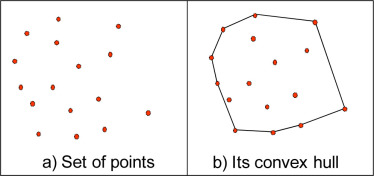
\includegraphics[width=0.8\textwidth]{Figures/convex hull.jpg}
	\caption{Convex Hull}
	\label{fig:convex hull}
\end{figure}

Table \ref{tab:Point Cloud Volume of Different Objects} shows the percentage error analysis from the computed volume of different model point cloud objects in the study of \citet{chang2017}, which shows that in order to estimate the volume of a shape represented by a point cloud, the area of each slice of the shape is calculated by finding the difference between the top and bottom curves of the slice. The total volume of the shape is then calculated by integrating the areas of all the slices using an integration interval equal to the length of the point cloud.

\begin{table}[H]
	\caption{Point Cloud Volume of Different Model}
	\label{tab:Point Cloud Volume of Different Objects}
	\centering
	\begin{tabular}{|c|c|c|c|}
		\hline
		% First row
		Objects        & True Value (\si{mm^3}) & Estimated Value (\si{mm^3}) & Error (\%) \\
		\hline
		% Second row
		Cube           & 1 000 000              & 1 000 000                   & 0          \\
		\hline
		% Third row
		Cylinder       & 125.664                & 125.061                     & 0.479      \\
		\hline
		% Fourth row
		Sphere         & 4 188 90.2             & 4 178 966.87                & 0.234      \\
		\hline
		% Fifth row
		Triangle Prism & 17.321                 & 17.399                      & 0.45       \\
		\hline
	\end{tabular}
\end{table}

The study conducted by \citet{jeong2018} introduces a newly developed explicit hybrid numerical methodology for 3D volume reconstruction from unorganized point clouds, which is based on a modified Allen-Cahn equation and a 3D binary picture segmentation method. The technique has demonstrated potential in a variety of practical applications, including 3D model printing from dispersed scanned data. The computational findings show that the suggested approach for reconstructing 3D volume from point clouds is very efficient and resilient.

\section{Robot Web Tools Application for ROS Remote Monitoring}

The integration of Robot Web Tools (RWT) with ROS has garnered significant attention in recent years due to its potential to revolutionize real-time robotics applications. By leveraging web technologies and cloud computing infrastructure, developers aim to create intuitive interfaces for controlling and monitoring robots remotely. Central to the capabilities of RWT is its efficient messaging mechanism, which enables real-time interaction between web-based interfaces and ROS-enabled robots. By leveraging technologies such as roslibjs and rosbridge, RWT facilitates the seamless exchange of data, including sensor readings, point clouds, and control commands. This efficient messaging paradigm forms the backbone of RWT's ability to provide responsive and interactive interfaces for controlling and monitoring robotic systems.

Several studies have explored the capabilities of RWT in enabling real-time interaction with ROS-enabled robots. For instance, in a study by \citet{qureshi2016poster}, the development of a disaster management application is showcased, wherein Robot Web Tools (RWT) is utilized for seamless communication with ROS nodes. This integration enables an efficient response to emergencies by facilitating real-time interaction and control of robots remotely.

Furthermore, \citet{lim2019cloud} explored the integration of ROS with cloud computing infrastructure to offload computationally intensive tasks and enhance scalability. They utilized RWT to develop web-based visualization tools for analyzing sensor data in real-time, showcasing its versatility in cloud robotics applications.

% The development of a measuring system for accurately defining grain surfaces led to the creation of a bin measurement system utilizing a laser distance meter, as described by \citet{turner2017}. According to the findings of the study, sophisticated data processing techniques were developed to simulate complicated grain surfaces, making it possible to estimate grain volume using the generated surface and bin geometry. However, the requirement for manual post-processing and visual examination restricted the automation of data processing. Moreover, the system's efficacy relied on a clear view of the entire grain surface \citep{turner2017}.

% \section{Point Cloud Processing}
% \label{rrl:sec:Point Cloud Processing}
% Recent advancements in 3D reconstruction and visualization based on point cloud data have led to rapid development in various fields due to the rich data information and detailed real-world representation of objects or environments. Consequently, this massive data, including enormous kinds of noise, is overwhelmingly tedious to manage \citep{li2020}.

% In the study conducted by \citet{wang2020}, when point cloud data are involved in construction applications, different point cloud data processing procedures are crucial to achieving desired outputs. Figure \ref{fig:data-processing} shows the common procedures for the raw point cloud data in a construction setting \citep{wang2020}.

% \begin{figure}[H]
% 	\centering
% 	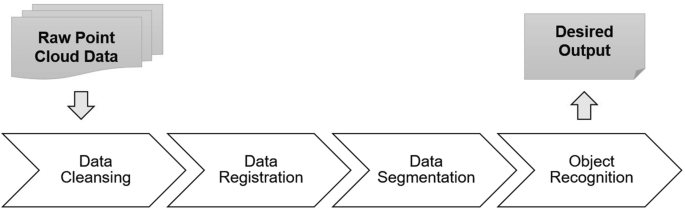
\includegraphics[width=0.9\textwidth]{data-processing}
% 	\caption{Typical processing procedures of point cloud data}
% 	\label{fig:data-processing}
% \end{figure}

% \citet{stanislas2021} divided the point cloud processing into four-step processes, figure \ref{fig:The-four-stages-of-the-point-cloud-classification-process} illustrates the structure of the authors, the point cloud output of the method is the same point cloud that was inputted before the classification took place. The method involves feature computing, data formatting, network prediction, and post-processing.

% \begin{figure}[H]
% 	\centering
% 	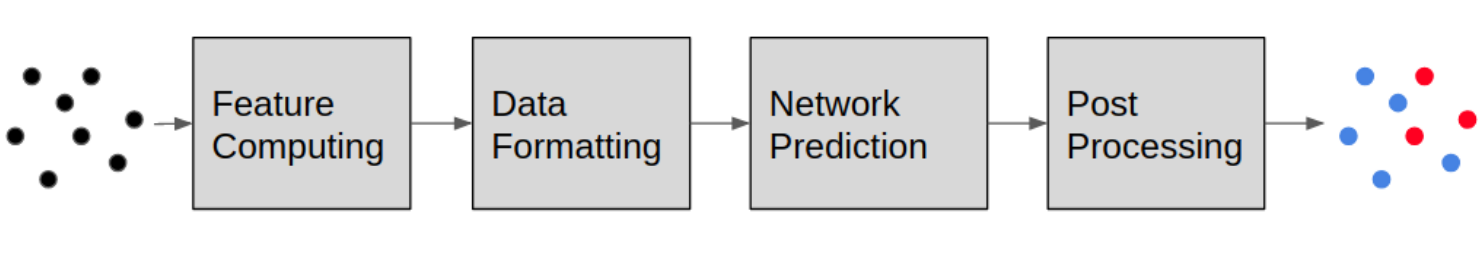
\includegraphics[width=\textwidth]{Figures/four-stage-of-pc-classification-process.png}
% 	\caption{The four stages of the point cloud classification process}
% 	\label{fig:The-four-stages-of-the-point-cloud-classification-process}
% \end{figure}

% \subsection{Outlier Point Cloud Processing}
% \label{sub:Point Cloud Processing}
% Processing of point cloud data by filtering is intensively exposed in research with a wide variety of applications. Cleaning of raw 3D point clouds is commonly the first step for most geometry processing, it involves removing the outliers (e.g., dust, snow, fog, etc.) after classifying the dust and non-dust (inliers) point cloud, smoothing the remaining data, and then reconstructing the surface into a three-dimensional representation \citep{rakotosaona2020}. Artificial Intelligence techniques such as Machine Learning (ML) and Deep Learning (DL) are widely used in classifying point cloud dust and non-dust data to remove noise.

% For instance, \citet{stanislas2018} detected dusty regions in point cloud data by using machine learning techniques as well as specialized neural networks. The 3D map was transformed into 3D occupancy grids in this investigation, and the occupied voxels were utilized to train classifiers based on machine learning to extract significant information, figure \ref{fig:pcl seg} shows the result of the study.

% \begin{figure}[H]
% 	\centering
% 	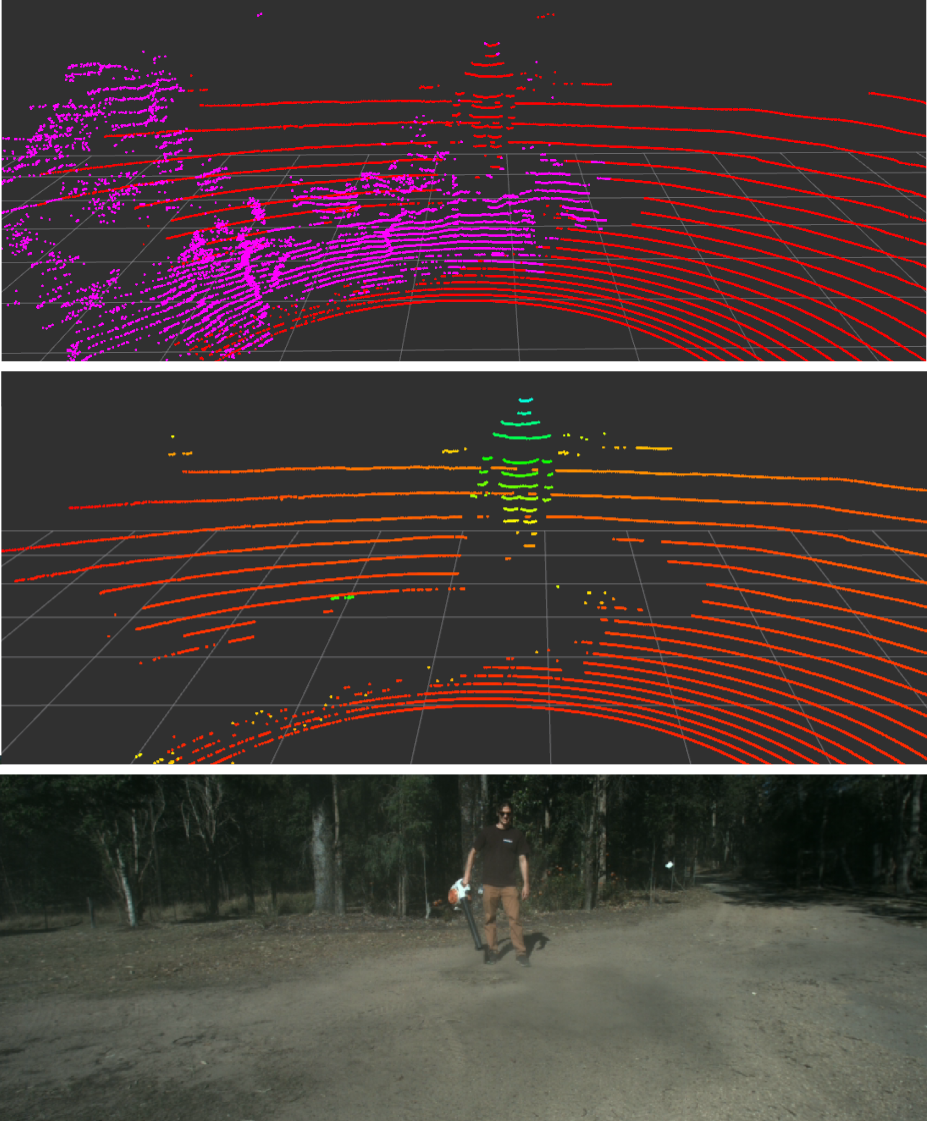
\includegraphics[width=0.7\textwidth]{pcl_seg}
% 	\caption{Top: Detection of airborne dust particle in a LiDAR point cloud, purple is Particle and red is Non-particle. Middle: Removal of detected dust particles from point cloud for robust perception, the color is mapped to the vertical axis (red is low, green is high). Bottom: Image depicting the scene.}
% 	\label{fig:pcl seg}
% \end{figure}

% The same voxel-based approach was also used in the study of \citet{shamsudin2016} for the classification of fog. The method involved using geometrical features and intensity as inputs for the support vector machine (SVM) and k-nearest neighbors (KNN) algorithms to classify fog.

% Both point- and voxel-based categorization were taken into account in study by \citet{stanislas2021}. They experimented with various classifier input features to determine the most effective one for dust removal in order to boost performance. These characteristics include geometry, intensity, and multi-echo data from the LiDAR sensor. With point-based deep learning techniques, geometry, and multi-echo features proved to be the most useful features, while voxel-based deep learning techniques benefited from the addition of intensity information to these features.

% To simplify the point cloud models and reduce the noise in point cloud data, \citet{zhu2020} employed the point-based simplification and guided filter. The guided filter was employed to filter the noisy point cloud model and generate the filtered image. The surface-based filtering group employs the filtering algorithm.

% \citet{ramiya2017} set a threshold by measuring the distance between every point and the mean surface. They assigned a weight to each point based on its distance from the interpolated mean surface.

% \citet{heinzler2020} used a large point cloud data set for CNN-based approach segmentation in controlled adverse weather effects. The approach takes a global understanding of the scene to estimate the validity of individual point measurements, rather than analyzing local spatial statistics as in previous approaches, it also proposes data augmentation technique that reduces the necessity for annotated ground truth data.

% The multi-echos and intensity data features of LiDAR point cloud are utilized in various studies. \citet{afzalaghaeinaeini2021} used low-intensity outlier removal (LIOR) filtering for de-dusting method. The method is composed of two procedures: First, dust particles based on point cloud usually have a lower intensity compared to non-dust point cloud, point cloud with an intensity lower than the set threshold are removed. Second,  the study successfully filtered the point cloud data and removed the dust from the original point cloud data.

% Intensity-based filter was also utilized by \citet{park2020} for removal of snow in point cloud data. The study concluded that this method overcomes the disadvantages of LiDAR sensor compared to other conventional filtering methods.

% \subsection{3D Space Point Cloud Mapping}

% In todays generation, various point cloud processing and mapping frameworks are widely available to lessen the complexity of handling raw point cloud data, such as, Robotic Operating System (ROS), Point Cloud Library (PCL), Open3D, MeshLab, etc. Most of this framework can be used in many different fields such as virtual reality, construction, industry, and surveying.

% The PCL has a built-in visualization library that uses Visualization ToolKit (VTK) as its foundation. VTK is a versatile platform that can render 3D point clouds and surfaces, and supports visualizing tensors, textures, and volumetric methods. The PCL Visualization library aims to merge PCL with VTK by providing a complete visualization layer for n-D point cloud structures. Its main goal is to allow for rapid prototyping and visualization of algorithm results on high-dimensional data \citep{rusu2011}.

% \citet{ocando2017} take advantage of using ROS framework to map the 3D point cloud data, as the framework allows to interlink programs that is written in different languages. The study successfully addressed the problematic tasks of Simultaneous Localization and Mapping (SLAM) and 3D Octomapping via single sensor.

% \section{Volume Estimation}
% \label{rrl:sec:Industrial Volume Measurement}
% Typically in an agriculture and food company setting, calculating the volume of a storage bin involves determining both the storage geometry and the distance between the grain surface and the eave. Traditionally, a fiberglass tape measure with weights is used to calculate the distance between the surface of the grain and the top of the bin. Correction factors are applied to the measurement to account for any irregularities in the surface of the grain, such as when the surface is uneven or when there is a cone-shaped pile \citep{turner2016}. These correction factors are usually simple to apply when the surface is relatively flat and equal in height. Moreover, these traditional approaches necessitate such effort and involved the employees to be at the top of the bin during the estimation. New methods and technologies have been trying to incorporate in industrial settings to eliminate these traditional methods such as using Microwaves Radar \citep{vogt2017}, Horn Antennas-based \citep{duysak2020, yigit2015}, Load Cell, Ultrasonic, Laser-based \citep{geuvara2020}, and Temperature-based sensor \citep{rhee2021}. Each of this technology has their own advantage and disadvantages, however, laser-based sensor (e.g. LiDAR) shows an interesting capabilities and features especially in acquiring three-dimensional point cloud data that can be used for geometric computation and for 3D object representation.

% Point clouds in 3D are highly valuable as they contain crucial information on the shape, size, area, and volume of objects. Various industries, including agriculture and fisheries, have effectively utilized volume estimating methods based on point clouds \citep{geuvara2020}.

% In computer graphics, a voxel is an image that depicts a specific region that has been partitioned into a grid of cubes that are all the same size and uniformly spaced \citep{putman2018}.

% Due to a better portrayal of the region encompassed in the group of points, the Delaunay triangulation and voxelization procedures outperform in estimating the outcomes. These strategies, however, have a greater computational cost because of their accuracy \citep{chee2015}. To estimate volume, methods such as Delaunay triangulation and voxelization are used. It is important to consider both accuracy and computing costs when using these methods. Height grids are faster for computing height discrepancies, but accuracy depends on precise point acquisition \citep{bewley2011, duff2000}.

% The Delaunay triangulation-based technique for volume computation, known as Delaunay triangulation-driven volume calculation (DTVC), differs from traditional approaches which computes the volume during the triangulation process rather than preserving Delaunay triangles. This method reduces both memory usage and processing time. Experimental findings demonstrate that DTVC achieves a satisfactory trade-off between precision and efficiency \citep{liuY2021}.

% Table \ref{tab:Point Cloud Volume of Different Objects} shows the percentage error analysis from the computed volume of different model point cloud objects in the study of \citet{chang2017}, which shows that in order to estimate the volume of a shape represented by a point cloud, the area of each slice of the shape is calculated by finding the difference between the top and bottom curves of the slice. The total volume of the shape is then calculated by integrating the areas of all the slices using an integration interval equal to the length of the point cloud.

% \begin{table}[H]
% 	\caption{Point Cloud Volume of Different Model}
% 	\label{tab:Point Cloud Volume of Different Objects}
% 	\centering
% 	\begin{tabular}{|c|c|c|c|}
% 		\hline
% 		% First row
% 		Objects        & True Value (\si{mm^3}) & Estimated Value (\si{mm^3}) & Error (\%) \\
% 		\hline
% 		% Second row
% 		Cube           & 1 000 000              & 1 000 000                   & 0          \\
% 		\hline
% 		% Third row
% 		Cylinder       & 125.664                & 125.061                     & 0.479      \\
% 		\hline
% 		% Fourth row
% 		Sphere         & 4 188 90.2             & 4 178 966.87                & 0.234      \\
% 		\hline
% 		% Fifth row
% 		Triangle Prism & 17.321                 & 17.399                      & 0.45       \\
% 		\hline
% 	\end{tabular}
% \end{table}

% The study conducted by \citet{jeong2018} introduces a newly developed explicit hybrid numerical methodology for 3D volume reconstruction from unorganized point clouds, which is based on a modified Allen-Cahn equation and a 3D binary picture segmentation method. The technique has demonstrated potential in a variety of practical applications, including 3D model printing from dispersed scanned data. The computational findings show that the suggested approach for reconstructing 3D volume from point clouds is very efficient and resilient.

% The Convex Hull is another method that is popular technique for measuring volume from 3D point cloud points (see figure \ref{fig:convex hull}). The computational geometry community has extensively studied the convex hull problem, as evidenced by the works of \citet{kim2002}, \citet{graham1983}, and \citet{maus1984}. Qhull is a commonly used algorithm to compute the convex hull, employing the Voronoi diagram, the Delaunay triangulation, furthest-site Voronoi diagram, the furthest-site Delauney triangulation, and the half-space intersection around a point. The software program allows the creation of high-dimensional objects, and the Quickhull algorithm, written in C, is used to compute the convex hull, which solves round-off errors in floating-point arithmetic. The program is capable of calculating volumes, surface areas, and convex hull approximations.

% \begin{figure}[H]
% 	\centering
% 	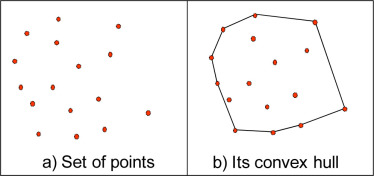
\includegraphics[width=0.8\textwidth]{Figures/convex hull.jpg}
% 	\caption{Convex Hull}
% 	\label{fig:convex hull}
% \end{figure}

\section{Synthesis of the Study}

The conducted review of related literature provides a comprehensive overview of existing methods, techniques, and technologies used for volume measurement, point cloud acquisition devices, and volume measurement using 3D point cloud data. It highlights the importance of enhancing post-harvest processing and storage technology to meet increasing global demand and minimize waste, emphasizing the role of advanced monitoring and management techniques in improving production efficiency and safety standards.

Various methods for volume measurement, including traditional level measurements and emerging technologies such as LiDAR, have been discussed. While traditional methods like weighted fiberglass tape provide a single data point, newer technologies offer more detailed and accurate measurements. Point cloud acquisition devices, particularly LiDAR, have emerged as powerful tools for generating detailed 3D models of objects or environments. Techniques for transforming 2D LiDAR scanners into 3D point cloud scanners have been explored, highlighting the use of rotating mechanisms and processing algorithms.

Additionally, the review discusses frameworks for point cloud processing, visualization, and mapping, emphasizing the importance of utilizing tools like ROS and PCL for efficient data handling. Techniques and methods for volume estimation using computational geometry, such as Delaunay triangulation and voxelization, have been examined, along with their applications in various industries.

Furthermore, the integration of Robot Web Tools (RWT) with ROS for remote monitoring of robots has been explored, demonstrating its potential in enabling real-time interaction and control of robots over the web. Several studies have demonstrated the capabilities of RWT in disaster management, cloud robotics, and real-time sensor data analysis.

Given the advancements in point cloud acquisition devices, volume measurement techniques, and web-based robotics interfaces, this study focused on integrating and utilizing these technologies and methods to provide an alternative solution to existing technology used in storage volume calculation. By leveraging existing technologies and methodologies, the aim of this study was to develop a feasible approach for enhancing storage technology especially in volume measurement technology.
\renewcommand{\thechapter}{\Roman{chapter}}
\chapter{Methodology}
\renewcommand{\thechapter}{\arabic{chapter}}
\label{ch4:Methodology}
\thispagestyle{empty}

In this chapter, the study discusses the systematic approach employed in the development of of the proposed system. As depicted in Figure \ref{ch4:fig:system_development_process}, each phases is essential in shaping the overall system functionality. This chapter explains the approach taken, giving an overview of the techniques, methods, and resources applied at every development step.

\begin{figure}[H]
	\centering
	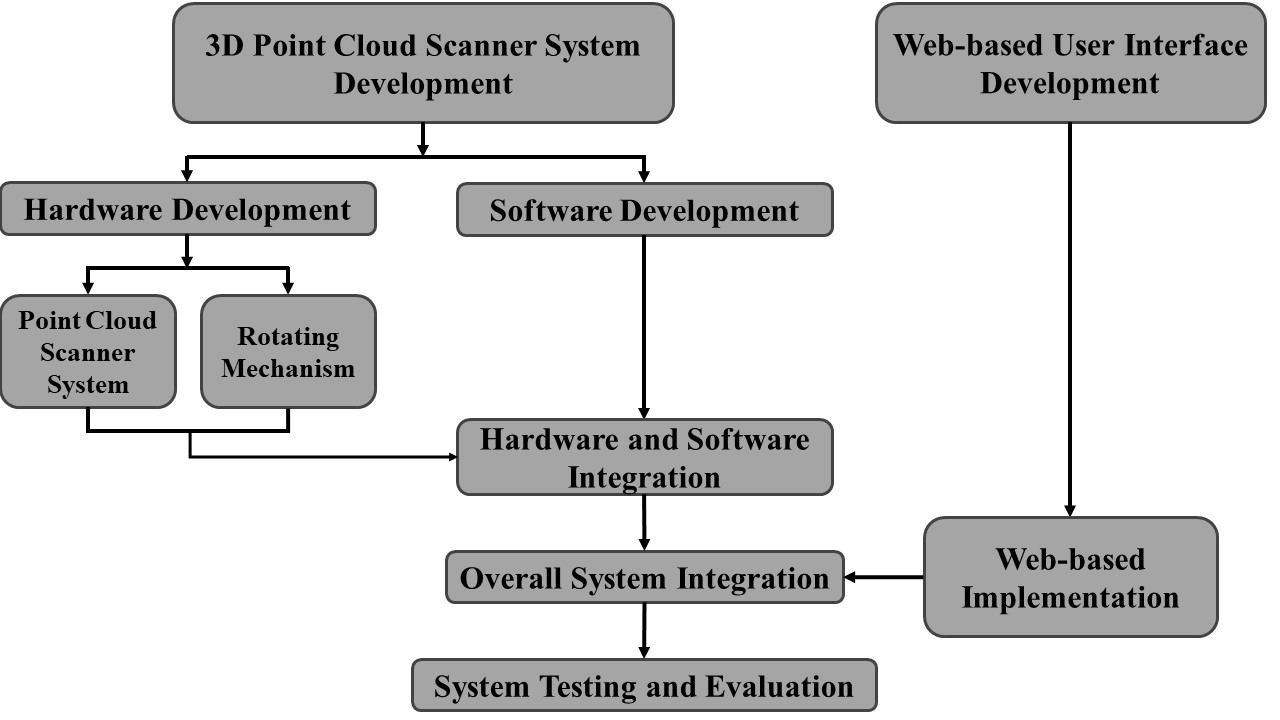
\includegraphics[width=1\textwidth]{Figures/system_development_process}
	\caption{System Development Process}
	\label{ch4:fig:system_development_process}
\end{figure}

\section{System Requirements Analysis}
\label{ch4:sec:system_requirements_analysis}

The development process of the study encompasses hardware, software, and web-based application design, followed by system integration and testing. As depicted in Figure \ref{ch4:fig:overall_system_setup_development} which is the proposed overall system setup, the study undertook the design and development of two distinct yet interconnected systems: the 3D Point Cloud Scanner (3D-PCSS), which is placed at the top of a storage bin, and the web-based application which is both connected to the local network. This overall system setup achieved by following a step by step development process which is illustrated in figure \ref{ch4:fig:system_development_process}, identifying hardware aspect which involves selecting and configuring the necessary components for data acquisition, processing, and communication. software development focuses on programming the processes to control hardware functionality and execute specific tasks. Meanwhile, web-based application design requires creating an interface for users to interact and data visualization. System integration involves bringing together these components and ensuring communication and functionality between them. Lastly, system testing and evaluation was conducted to validate the functionality, performance, and reliability of the developed systems through various testing procedures.

\begin{figure}[H]
	\centering
	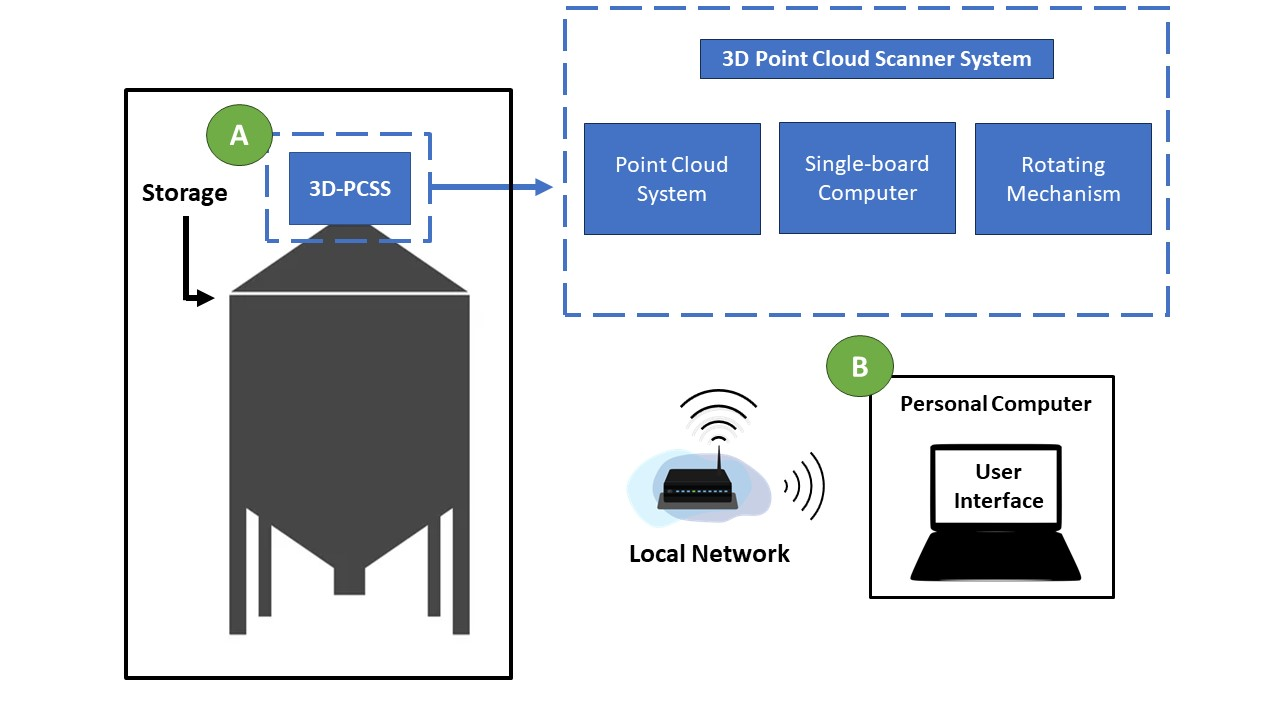
\includegraphics[width=1\textwidth]{Figures/system_analysis}
	\caption{Overall System Setup: (A) 3D-PCSS, (B) User Interface}
	\label{ch4:fig:overall_system_setup_development}
\end{figure}

\section{Hardware Development}
\label{ch4:sec:hardaware_design}

The hardware development conducted in this study involves the design and construction of 3D point cloud scanner and storage bin. The storage bin was created for testing and evaluation of the overall system.

% The researcher will adopt the concept of tilting method using a 2D of-the-shelf LiDAR to acquire 3D point cloud data to minimize the cost compared to commercial 3D LiDAR. The hardware and physical components of 3D point cloud scanner are composed of three major components, the 2D LiDAR device, the tilting mechanism which include the fabricated holder for mechanical tilting and the motor for the rotation movement. In Figure \ref{ch4:fig:System Hardware Block Diagram}, the 3D point cloud scanner is placed at the top of the flour bin.

% \begin{figure}
% 	\centering
% 	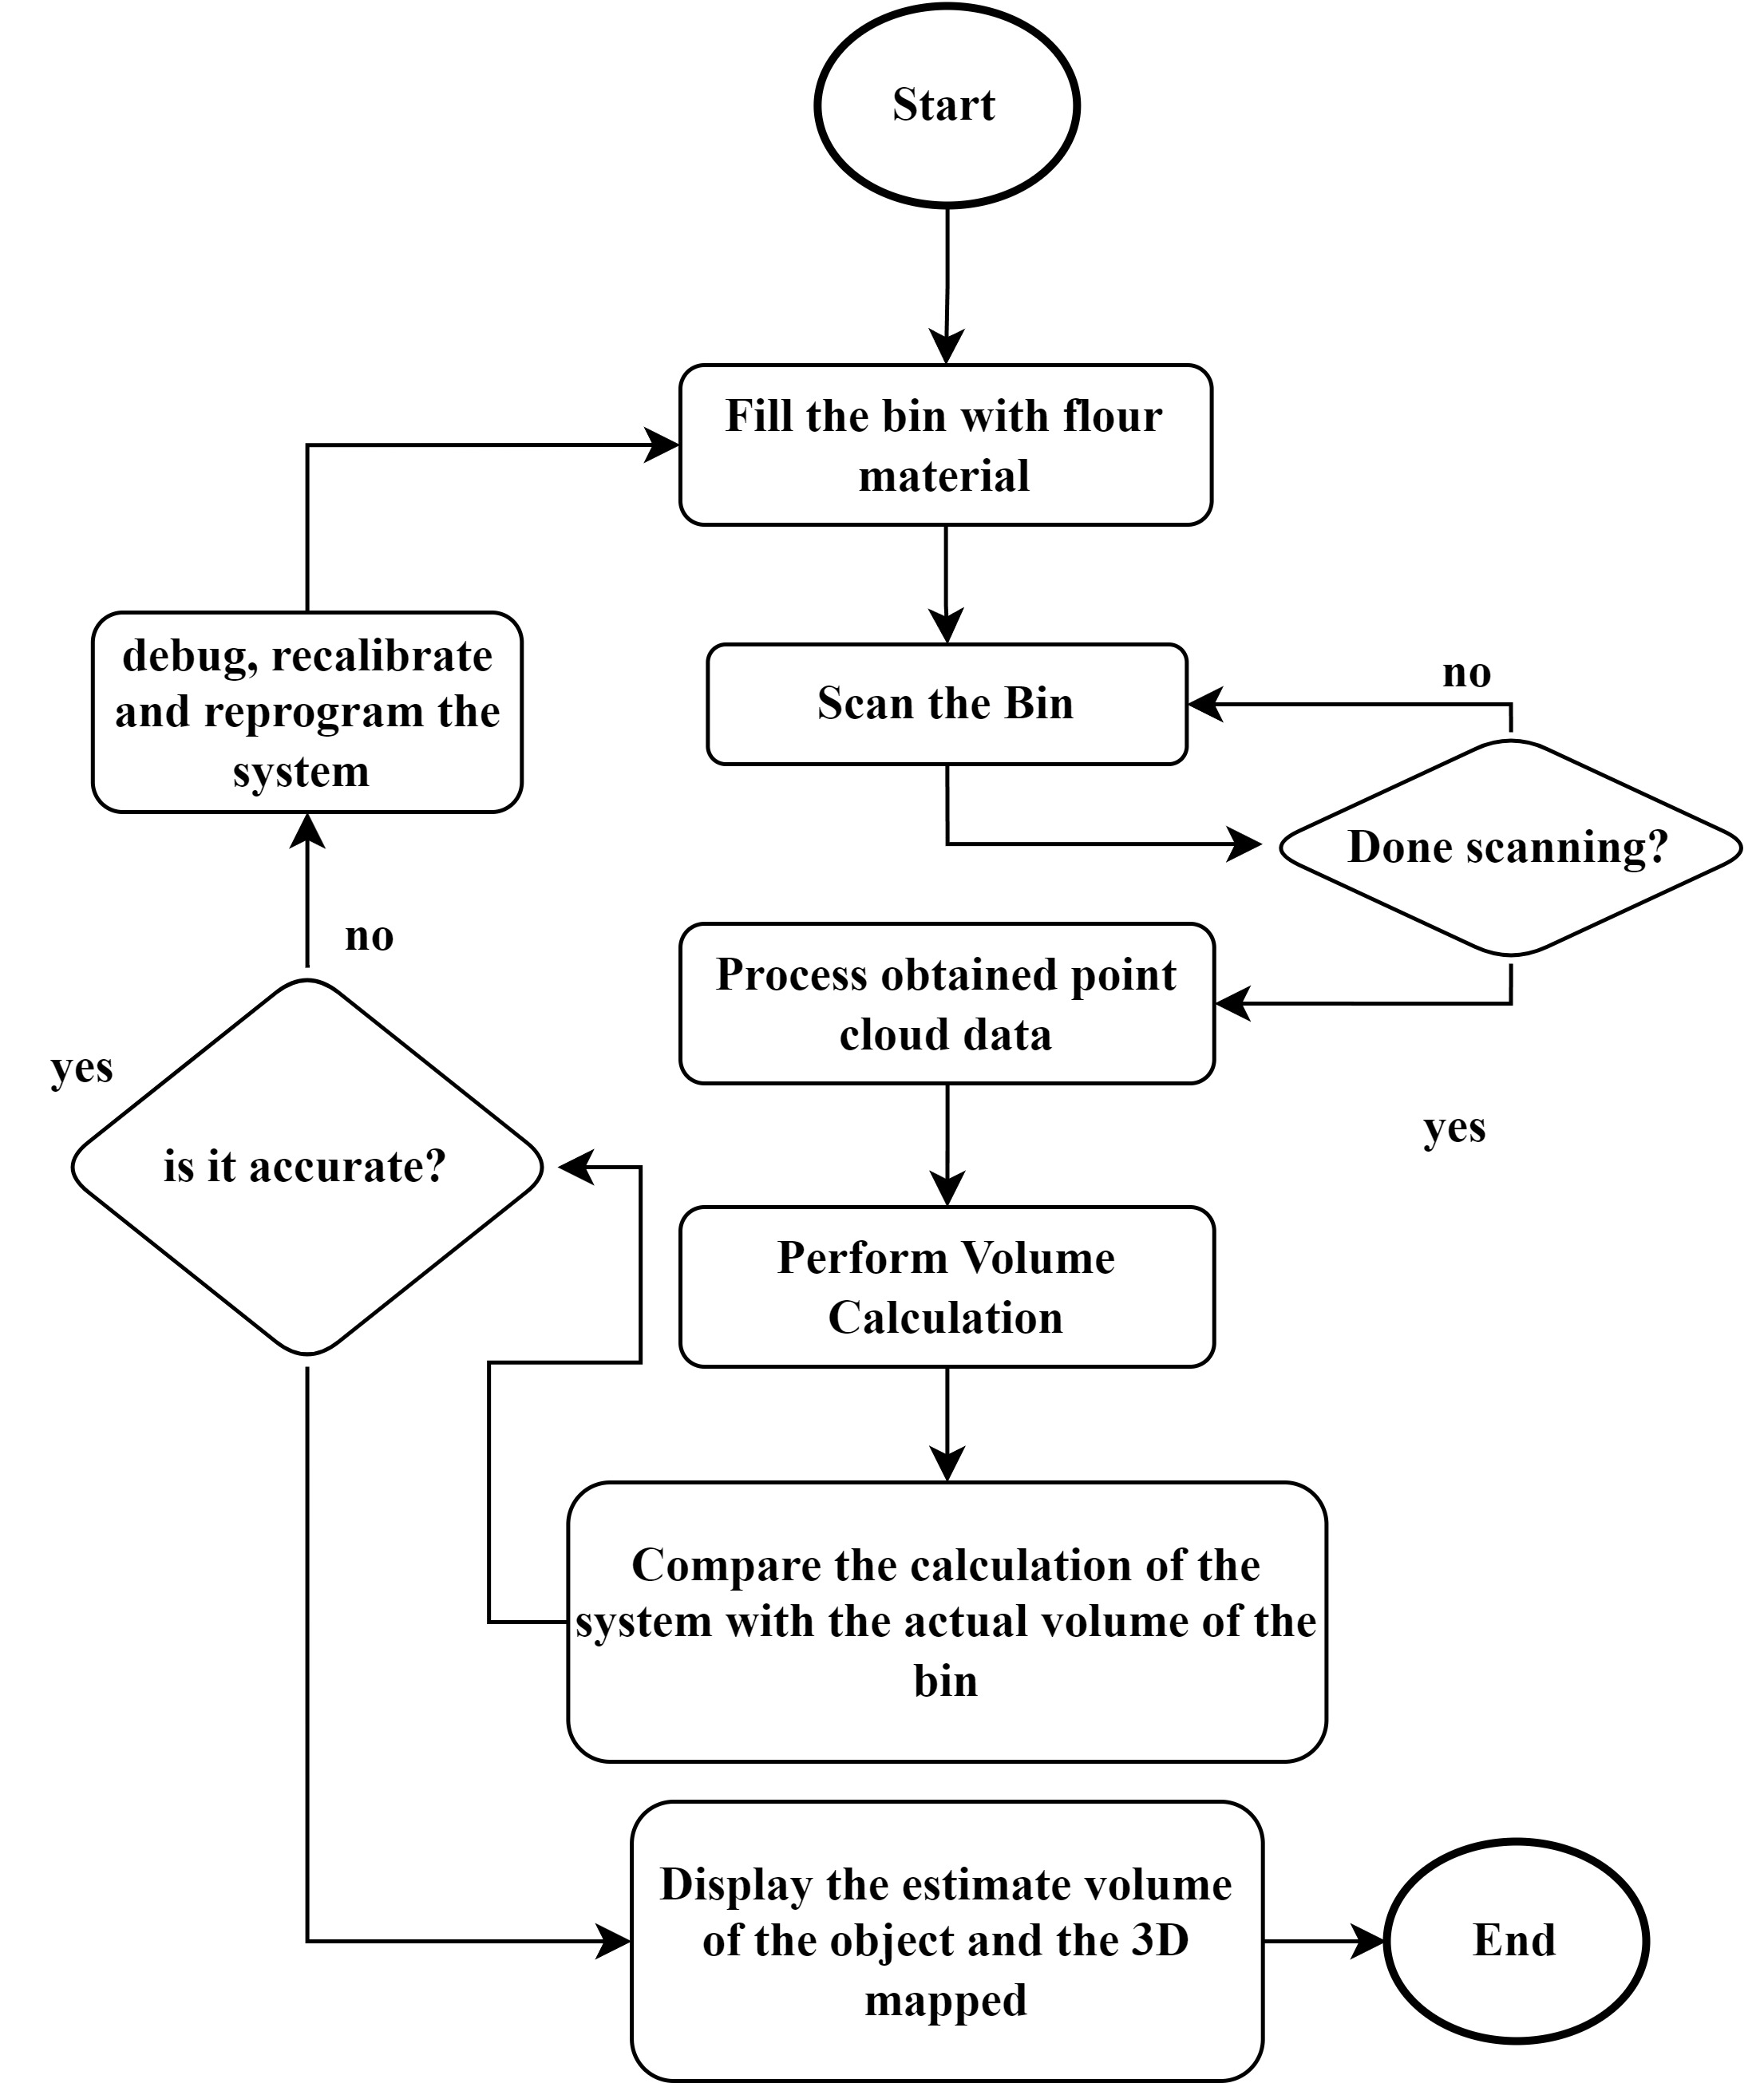
\includegraphics[width=0.9\textwidth]{Figures/general-flowchart-of-the-system-2.jpg}
% 	\caption{General Flowchart of the System}
% 	\label{ch4:fig:General flowchart of the system}
% \end{figure}

\subsection{Creating a Storage Bin}
\label{ch4:subsec:Modeling of Flour Bin}
The study involves constructing a mock-up flour storage bin modeled after those commonly used in food manufacturing industries. The mock-up bin is designed to closely mimic the geometric shape and proportions of real storage bins used in practice.

\subsection{3D Point Cloud Scanner Design (3D-PCSS)}
\label{ch4:subsec:3d_point_cloud_scanner_design}

\subsubsection*{Point Cloud Scanner System}

Point cloud devices, such as LiDAR (Light Detection and Ranging), offer exceptional accuracy in acquiring distance measurements over considerable distances. LiDAR systems emit laser pulses and measure the time it takes for these pulses to return after bouncing off objects in the environment. This technology enables the creation of highly detailed and accurate three-dimensional point clouds, which represent the surfaces and structures within the scanned area. Even low-cost LiDAR options are available in the market, making this technology accessible for various applications and budgets.

The point cloud scanner system in this study used a low-cost 2D LiDAR device controlled with single-board computer (SBC) for its computing functionality. \\

\subsubsection*{Rotating Mechanism}

The rotating mechanism design which is attached to the 2D LiDAR in this study is based on the methodology outlined in a previous research conducted by \citet{clar2022}. This prior study served as a foundational framework for the development of the rotating 2D LiDAR system in this study, providing into the integration of a pan-tilt unit (PTU) with a 2D LiDAR scanner to enable three-dimensional point cloud scanning. By employment the principles and techniques conducted in \citet{clar2022}, the current study aims to further refine and enhance the performance of the rotating 2D LiDAR system for its intended application and also address the problem encountered in the previous study.

The servo motor utilized in this study was the AX-12A Dynamixel, known for its high precision and reliability in robotic applications. What sets this servo apart is its compatibility with a Software Development Kit (SDK), which includes configurations for integration with the Robot Operating System (ROS). This feature enables communication and control of the servo motor within the ROS ecosystem, allowing for flexible and efficient development of robotic systems. This feature enables the LiDAR and Servo to communicate and synchronize, figure \ref{ch4:fig:servo_lidar_comm} shows the synchronization of the LiDAR and servo. \\

% \begin{algorithm}[]
% 	\caption{LDA}
% 	\label{ch4:algo:servo_and_lidar}
% 	\begin{algorithmic}[1]
% 		\FOR{$d$}
% 		\STATE{
% 			\FOR{$k\in\{1,...,K\}$}
% 			\STATE{Generate$\beta_k=(\beta_{k_1},...,\beta_{k,V})^T \sim Dirichlet(\cdot\vert\eta)$}
% 			\ENDFOR
% 		}
% 		\ENDFOR
% 	\end{algorithmic}
% \end{algorithm}

\begin{figure}[H]
	\centering
	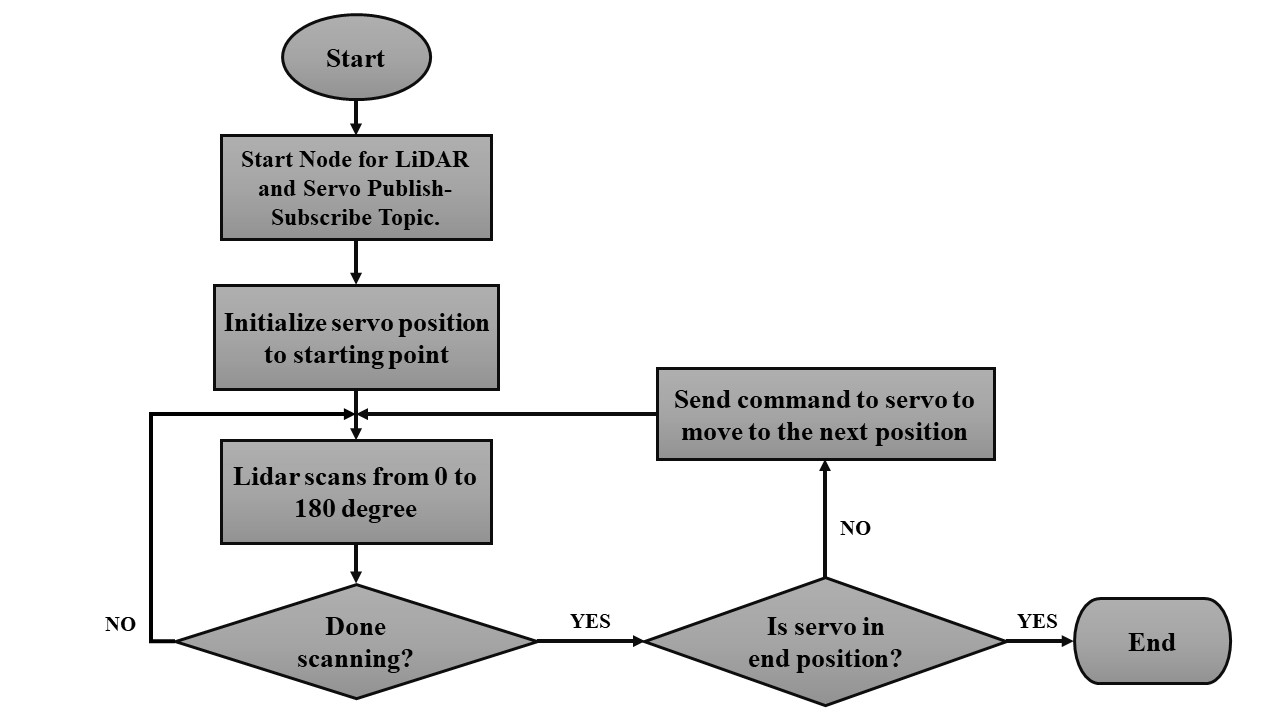
\includegraphics[width=1\textwidth]{Figures/servo_lidar_comm}
	\caption{Synchronization Process of LiDAR and Servo}
	\label{ch4:fig:servo_lidar_comm}
\end{figure}

The 3D-PCSS is the integration of point cloud scanner system and rotating mechanism. The major components of the system is illustrated in the figure \ref{ch4:fig:components_of_3d-pcss}, the hardware design flow chart of the system is shown in figure \ref{ch4:fig:3d-pcss_development_flow_chart}. The 3D-PCSS in this study considers the following design and functionality:
\begin{itemize}
	\item Based on low-cost 2D LiDAR device.
	\item Able to establish the communication between the rotating mechanism and LiDAR device.
	\item Able to gather and process 3D point cloud data.
	\item Support for connecting to a local network for remote data visualization and monitoring.
	\item Utilizing Robot Operating System (ROS) and Point Cloud Library (PCL) for its firmware development.
\end{itemize}

\begin{figure}[H]
	\centering
	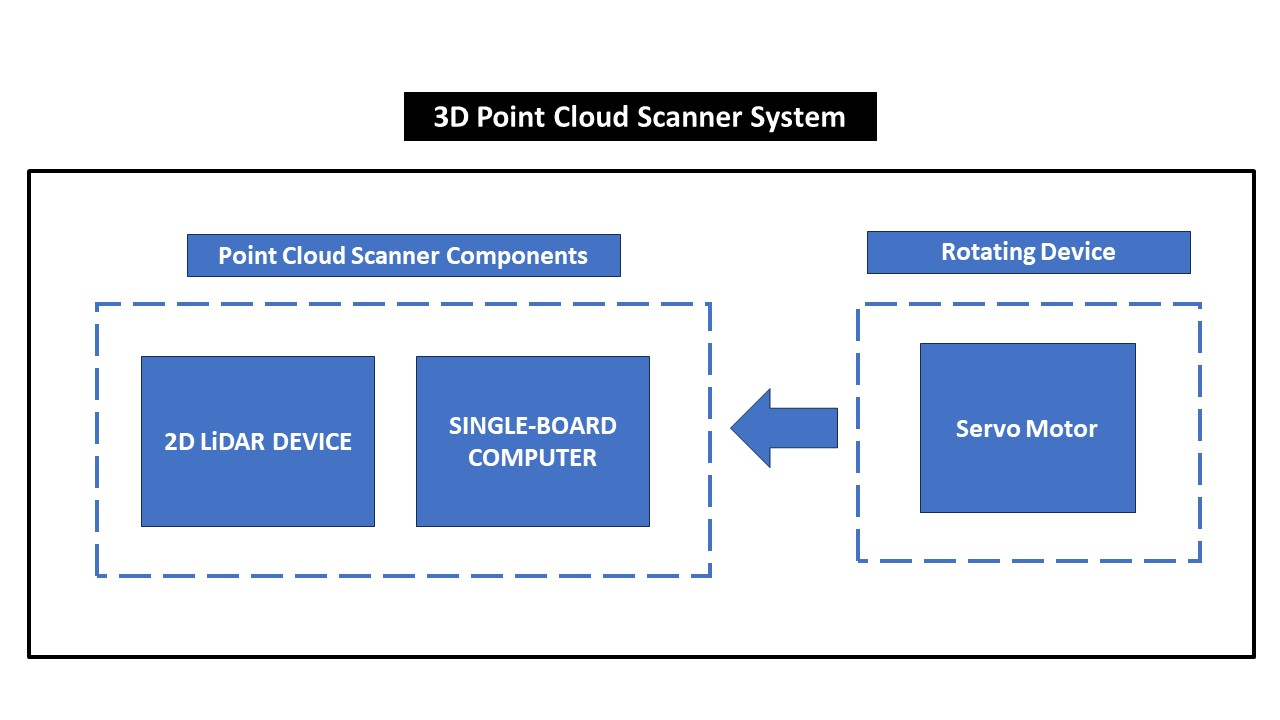
\includegraphics[width=1\textwidth]{Figures/3D-PCSS components}
	\caption{Major Components of 3D-PCSS}
	\label{ch4:fig:components_of_3d-pcss}
\end{figure}

\begin{figure}[H]
	\centering
	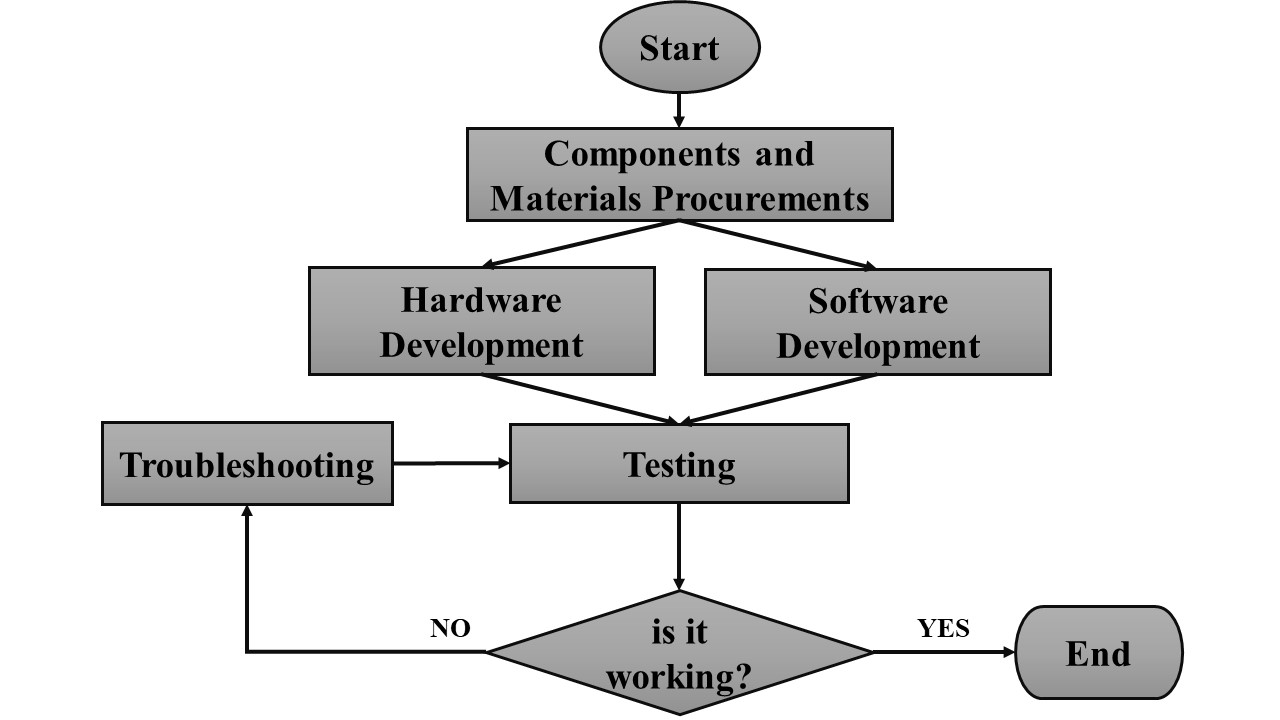
\includegraphics[width=0.8\textwidth]{Figures/hardware_flowchart}
	\caption{Hardware Design Flow Chart}
	\label{ch4:fig:3d-pcss_development_flow_chart}
\end{figure}

% \subsection{Data Gathering}
% For the data gathering of the raw point cloud, all the major hardware of the system will be assemble and integrate as shown in Figure \ref{ch4:fig:System Hardware Block Diagram}. The scanned data from the 2D LiDAR sensor will be received by small computer which is Raspberry Pi for the processing of the raw data. This small computer is connected to the internet in order to control remotely by the personal laptop. Different scanning procedure will be performed to gather point cloud data.

% \begin{figure}[H]
% 	\centering
% 	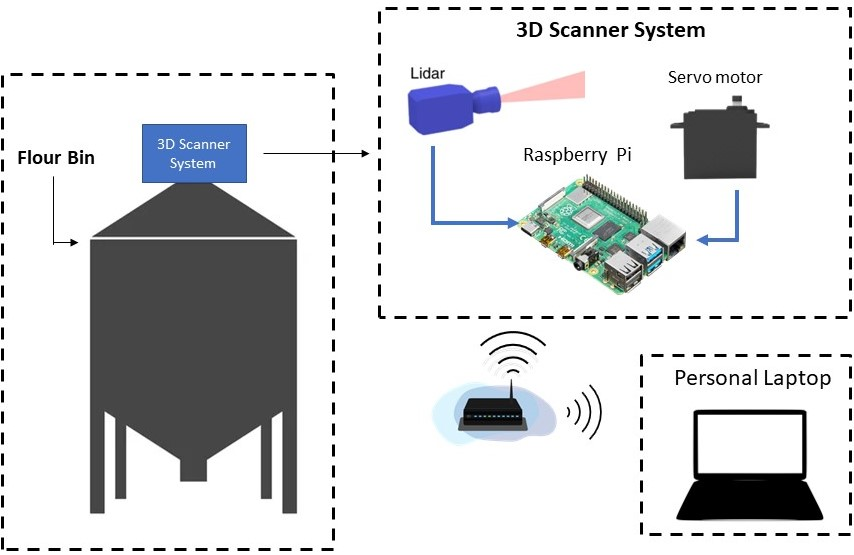
\includegraphics[width=0.9\textwidth]{Figures/system-hardware-block-diagram.jpg}
% 	\caption{System Hardware Block Diagram}
% 	\label{ch4:fig:System Hardware Block Diagram}
% \end{figure}

\section{Software Development}
\label{ch4:sec:firmware_development_design}

Software design plays a crucial role in the development of the 3D-PCSS by facilitating communication between hardware components, and allows connection with external software system. The system was designed to initialize all necessary components, including nodes and connection, immediately upon power-up. This ensures seamless operation and also establish connection with the developed web application for user interaction. As described in figure \ref{ch4:fig:software_system_process}, after turning on the system, it initializes essential nodes and enter in idle mode waiting for an external command coming from the web application. The system remain in idle mode unless turnoff. The development of software processes, including the choice of operating system and frameworks is outlined in this section.

Throughout this study, it's important to note that the terms 'process' and 'nodes' are used interchangeably. This interchangeable usage highlights the fundamental concept in ROS where processes, represented as nodes, perform computation and communication tasks within the system.

\begin{figure}[H]
	\centering
	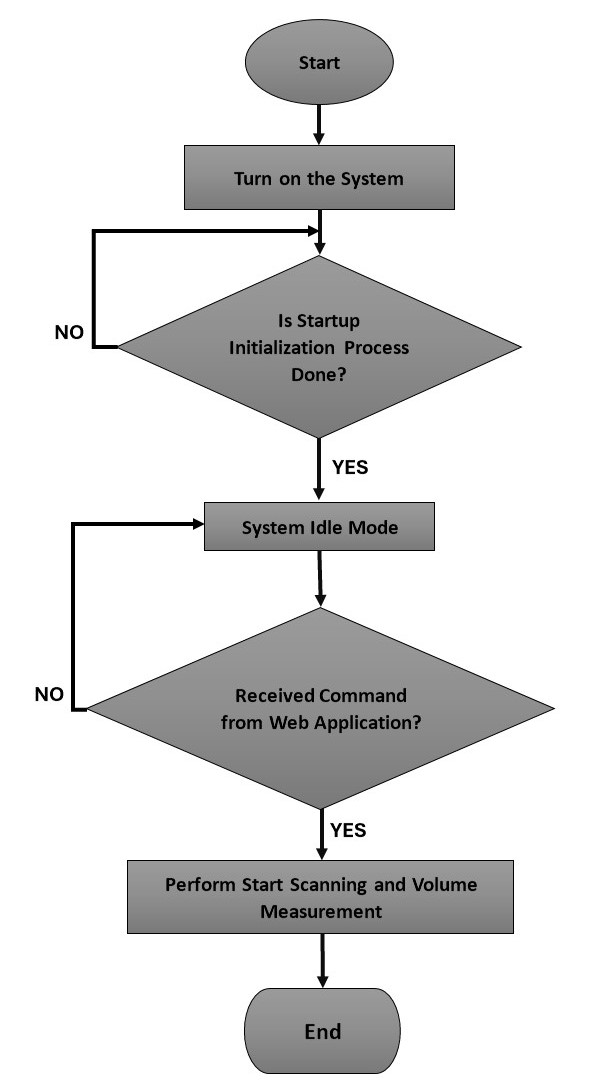
\includegraphics[width=0.7\textwidth, height=0.7\textheight]{Figures/software_system_process}
	\caption{System Process Flow Chart}
	\label{ch4:fig:software_system_process}
\end{figure}

\subsection{Operating System and Frameworks}

In this study, the single-board computer (SBC) used in the 3D-PCSS requires an appropriate OS and frameworks to support the execution of firmware and software components. Linux-based operating systems, such as Ubuntu, is commonly chosen for SBCs due to its reliability, flexibility, and extensive community support. This OS option provide a stable platform for running Robot Operating System (ROS) nodes and managing system resources effectively, thus, was utilized in this study. ROS framework was also utilized in this study to develop a publish-subscribe relationship between ROS nodes. Lastly, Point Cloud Library (PCL) serves in this study as a fundamental library being used for processing and analyzing point cloud data. PCL provides a comprehensive set of algorithms and tools for tasks such as point cloud registration, filtering and computational geometry to name a few.

\subsection{Startup Initialization Process}
Roscore and rosgridge are the two essential cores that used in the 3D-PCSS. These cores or nodes typically need to be manually started in the command-line interface (CLI) or desktop environment to run and process data, or to initiate other nodes and do specific tasks. In this study, a custom service file was developed to automate and start these nodes after the system is turnon. This file is created using Linux systemd to configure and instantly run the necessary programs or nodes.

% The Raspberry Pi will receive the scanned raw data coming from the 3D point cloud scanner. This data will be processed in different stages to produced desired output, such as point cloud pre-processing (formatting, converting, clustering, and cleansing) and post-processing (e.g., 3D mapping and volume measurement). Various platforms and frameworks nowadays are available to ease the handling of these massive raw data, thus, formatting the data to a desired platform must be perform. Typically, the value of raw data coming from the LiDAR sensor is not directly a point cloud data but rather a value of the distance between the sensor and the reflected nearest object in a particular direction, therefore, the data is converted into point cloud which composed of x, y, and z values. The Equation \eqref{ch4:eq:x-point}, \eqref{ch4:eq:y-point}, and \eqref{ch4:eq:z-point} is conversion of polar coordinates (distance, angle) to cartesian coordinates x, y, and z, respectively, in a 3D coordinate system.

% \begin{equation}
% 	x_{point_{i}} = \ \sin(i) \times d \
% 	\label{ch4:eq:x-point}
% \end{equation}
% \begin{equation}
% 	y_{point_{i}} = \ \cos(\pi) \times \cos(i) \times d \
% 	\label{ch4:eq:y-point}
% \end{equation}
% \begin{equation}
% 	z_{point_{i}} = \ -\cos(i) \times \sin(\pi) \times d \
% 	\label{ch4:eq:z-point}
% \end{equation}

% Where:

% \indent \indent i = scan angle of the scanner

% \indent \indent d = the distance point of the emitted pulse by the LiDAR (meter)

\subsection{System Scanning and Point Cloud Processes}

The researcher will create an algorithm for clustering and cleansing of the raw data. The data will be clustered into two parts, the outliers (dust) data and the inliers (target) data. Based on the behaviors and characteristics of dust, the researcher will use the Multi-echo method for outlier clustering because the laser emitted by the LiDAR will penetrate through the dust cloud and will receive multiple return. Another method that the researcher will utilize is the low-intensity method clustering for outliers due to the characteristic of the dust having a lower intensity compared to other objects. The data cleansing will be employed after all the data is being clustered. After of these processes, the researcher will convert the pre-processed point cloud for further analysis.

\subsection{Volume Estimation}
\label{ch4:sec:Volume Estimation}
The researcher will create an algorithm for volume estimation of the material inside the flour bin using Delaunay Triangulation which creates a mesh of triangles such that no point is inside the the circumference of any of the triangle. Convex Hull is a subset of Delaunay Triangulation which creates a boundary on the same given points, all the triangles are on the boundary of the point set. The computation of the estimated volume of the material inside the bin is shown in Figure \ref{ch4:fig:volume-estimation-figure} and Equation \eqref{ch4:eq:volume-estimation}.

\begin{figure}[H]
	\centering
	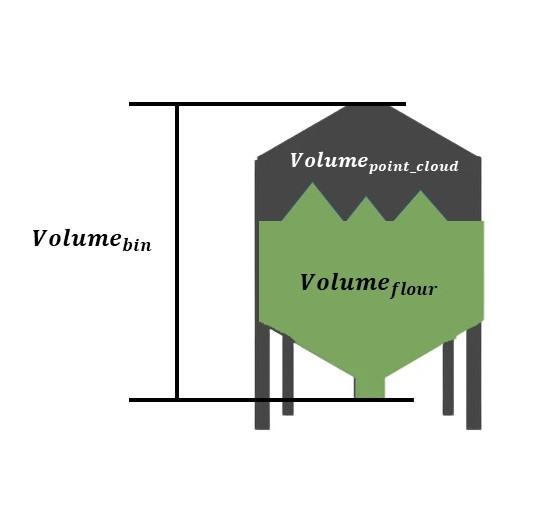
\includegraphics[width=0.8\textwidth]{Figures/volume-estimation-figure}
	\caption{Volume of the flour is the difference between the volume of the bin and volume of the point cloud}
	\label{ch4:fig:volume-estimation-figure}
\end{figure}

\begin{equation}
	Volume_{flour} = Volume_{bin} - Volume_{point\_cloud}
	\label{ch4:eq:volume-estimation}
\end{equation}

\section{Web-based Application Development}
This custom user interface based on web application is developed to used for the 3D-PCSS. The tools, framework and and resources of the system is discussed in this section.

The user interface consider the following design and functionality, the UI should be:
\begin{itemize}
	\item Intuitive and simple.
	\item Able to establish connection to the 3D-PCSS.
	\item Able to send command, display 3D point cloud data and volume measurement.
\end{itemize}

\section{Overall System Testing and Evaluation}
\label{ch4:sec:Testing and Evaluation}
In this section, Different testing was conducted

\subsection{Different Testing Procedure}
\label{ch4:subsec:Different Testing Procedure}
The researcher will conduct different testing and evaluation to observe the accuracy of the system. In the experiment, the researcher will ensure that the prototype flour bin is scanned remotely and without any human intervention. The researcher intends to perform multiple tests to assess the filtering method and validate the precision and effectiveness of the object's volume measurement, and each of the testing will have a multiple trials. The different testing procedure of the system are the following:
\begin{enumerate}
	\item \label{ch4:first} The system will scan the created different shape of flour bin without materials and dust inside.
	\item \label{ch4:second} The researcher will generate a dust in the flour bin but without material inside and scan the bin.
	\item \label{ch4:third} The searcher will scan the flour bin with flour material inside with different surface shape but without dust.
	\item \label{ch4:fourth} The researcher will generate dust from the testing structure conducted in testing \ref{ch4:third}
\end{enumerate}

\subsection{Evaluation of the System}
\label{ch4:subsec:Evaluation of the System}
Based on the conducted different testing mentioned in \ref{ch4:subsec:Different Testing Procedure}, the researcher will evaluate the conducted testing based on the volume of scanned data. System in the following evaluation

To evaluate the testing \ref{ch4:first}, the researcher will measure the accuracy of the system by comparing the estimated volume of the system  with the actual volume of the different shape of the bin, calculate the error percentage for each trial and assess the over all precision of the system. Table \ref{ch4:tab:Testing 1} shows the sample comparison of the testing.

\begin{table}[H]
	\caption{Testing \ref{ch4:first}}
	\label{ch4:tab:Testing 1}
	\centering
	\begin{tabular}{|c|c|c|c|}
		\hline
		% First row
		Flour bin Shape & Actual Volume (\si{mm^3}) & Scanned Volume (\si{mm^3}) & Error (\%) \\
		\hline
		\multicolumn{4}{|c|}{Trial 1}                                                         \\
		\hline
		% Second row
		Cube            & -                         & -                          & -          \\
		\hline
		% Third row
		Cylinder        & -                         & -                          & -          \\
		\hline
		\multicolumn{4}{|c|}{Trial 2}                                                         \\
		\hline
		Cube            & -                         & -                          & -          \\
		\hline
		% Third row
		Cylinder        & -                         & -                          & -          \\
		\hline
	\end{tabular}
\end{table}

Testing \ref{ch4:second} will be evaluated from the testing \ref{ch4:first} based on the number of point cloud acquired of both testing, and compare it. Basically, the testing \ref{ch4:second} will acquired more point cloud compared to testing \ref{ch4:first} due to multi-echo or multiple returning from the dust and the flour bin.

In testing \ref{ch4:third} and \ref{ch4:fourth}, the researcher will place flour materials inside the bin with different surface shape and perform volume estimation. After the volume estimation, the researcher will generate dust, scan the bin, perform volume estimation and compare it to the result of the testing \ref{ch4:third}. The sample result of testing \ref{ch4:third} and \ref{ch4:fourth} is shown in table

\begin{table}[H]
	\caption{Testing 3 and 4}
	\label{ch4:tab:Testing 3 and 4}
	\centering
	\begin{tabular}{|c|p{0.27\linewidth}|p{0.26\linewidth}|p{0.2\linewidth}|}
		\hline
		% First row
		Flour bin Shape & Scanned Volume (without dust) & Scanned Volume (with dust) & Error (\%) \\
		\hline
		\multicolumn{4}{|c|}{Surface Shape 1}                                                     \\
		\hline
		% Second row
		Cube            & -                             & -                          & -          \\
		\hline
		% Third row
		Cylinder        & -                             & -                          & -          \\
		\hline
		\multicolumn{4}{|c|}{Surface Shape 2}                                                     \\
		\hline
		Cube            & -                             & -                          & -          \\
		\hline
		% Third row
		Cylinder        & -                             & -                          & -          \\
		\hline
	\end{tabular}
\end{table}
\renewcommand{\thechapter}{\Roman{chapter}}
\chapter{Result and Discussion}
\renewcommand{\thechapter}{\arabic{chapter}}
\label{ch:Result and Discussion}
\thispagestyle{empty}

The results of the system development outlined in the previous chapter were presented and discussed in this chapter. After evaluating the specification of each system and undergo different design revision and integration, the study successfully identified and finalized the necessary components, tools and materials for each system.

\section{Developed 3D Point Cloud Scanner System (3D-PCSS)}

\subsection{3D-PCSS CAD Design Setup}

The 3D Point Cloud Scanner System hardware setup, as shown in Figure \ref{ch4:fig:cad_storage_bin}, consists of a 2D LiDAR Device fixed to a platform connected to a servo motor. This servo motor allows the platform to rotate, giving the LiDAR device an extra axis of movement. Inside the compartment is where the single-board computer along with other circuit components located. The detailed specification of each of the components is presented in appendix \ref{appen:a}.

\begin{figure}[H]
	\centering
	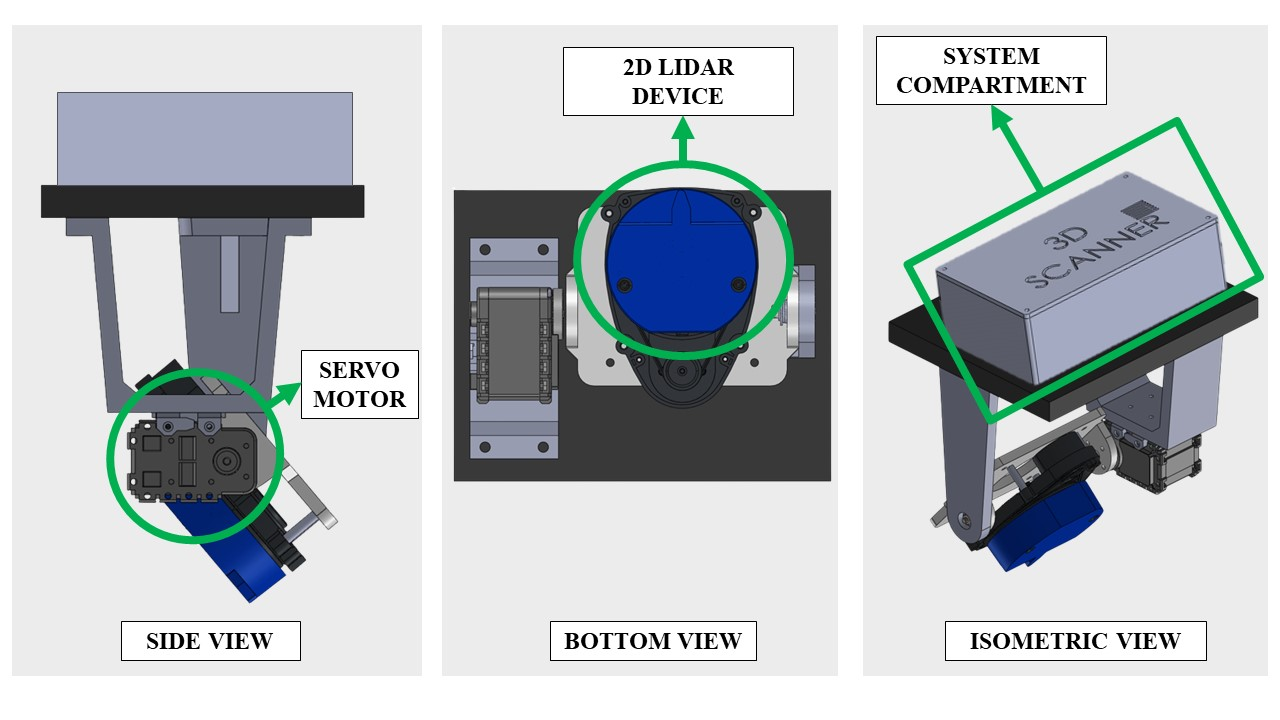
\includegraphics[width=1\textwidth]{Figures/3d-pcss-cad-design}
	\caption{Different View of the CAD Model Design of 3D-PCSS}
	\label{ch4:fig:cad_storage_bin}
\end{figure}

\subsection{Actual Design of the 3D-PCSS}

The actual development of the 3D-PCSS shown in figure \ref{ch4:fig:actual-3d-pcss} was constructed in accordance with the 3D CAD model design and the system is powered by a battery. Before the integration of the system, individual component testing were conducted to test and verify if such components function properly. The base platform, to which the 2D LiDAR device and servo motor are attached, was fabricated using aluminum metal. The system compartment is fabricated using a 3D printer and employing ABS material. Inside the compartment, the specific components and its category is shown in figure \ref{ch4:fig:specific-components}
\begin{figure}[H]
	\centering
	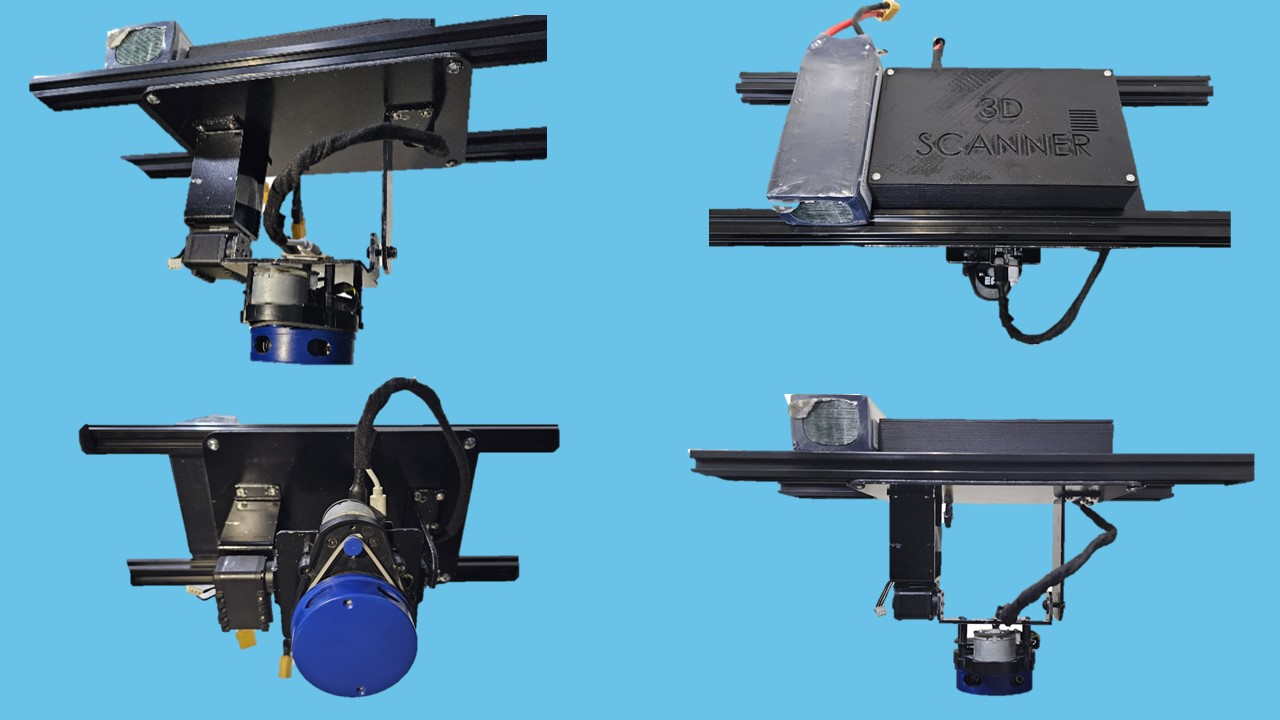
\includegraphics[width=1\textwidth]{Figures/actual-3d-pcss}
	\caption{Actual 3D-PCSS Developed}
	\label{ch4:fig:actual-3d-pcss}
\end{figure}

\begin{figure}[H]
	\centering
	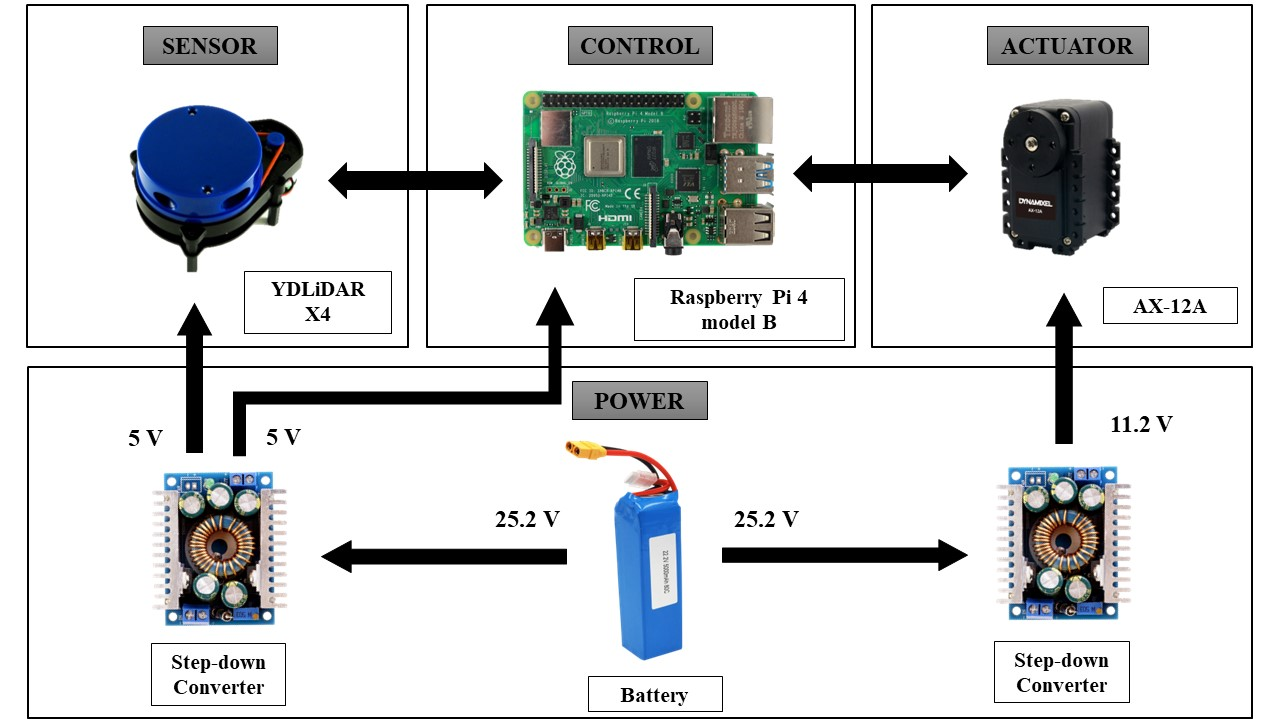
\includegraphics[width=1\textwidth]{Figures/specific-components}
	\caption{Specific Components of the System}
	\label{ch4:fig:specific-components}
\end{figure}

\section{Software Implementation}

The processes discussed in the previous chapter were implemented on the single-board computer (Raspberry Pi), playing a crucial role in the overall functionality of the 3D-PCSS. Figure \ref{ch4:fig:nodes-topics-relationships} illustrates the various nodes, topics, and their relationships in a publish-subscribe model. This implementation were apply after construction of the actual design of the 3D-PCSS. The arrows in the diagram show how data flows between the different nodes and its relationship to a corresponding topics. The ROS bridge server Node facilitates communication by relaying commands between the web application and the ROS framework via the ``/rosapi" service. Commands to start and stop scanning from the web interface are processed using the Remote Command Node within the system. The LiDAR Node captures data and publishes it as range values, while the Dynamixel Node and LiDAR Node synchronize their operations through the ``/dxl\_pos" topic. The Scan to 3D Point Cloud Mapping Node converts raw scan data into usable 3D point cloud data. Finally, the post-processing stage refines the point cloud data for volume measurement.

\begin{figure}[H]
	\centering
	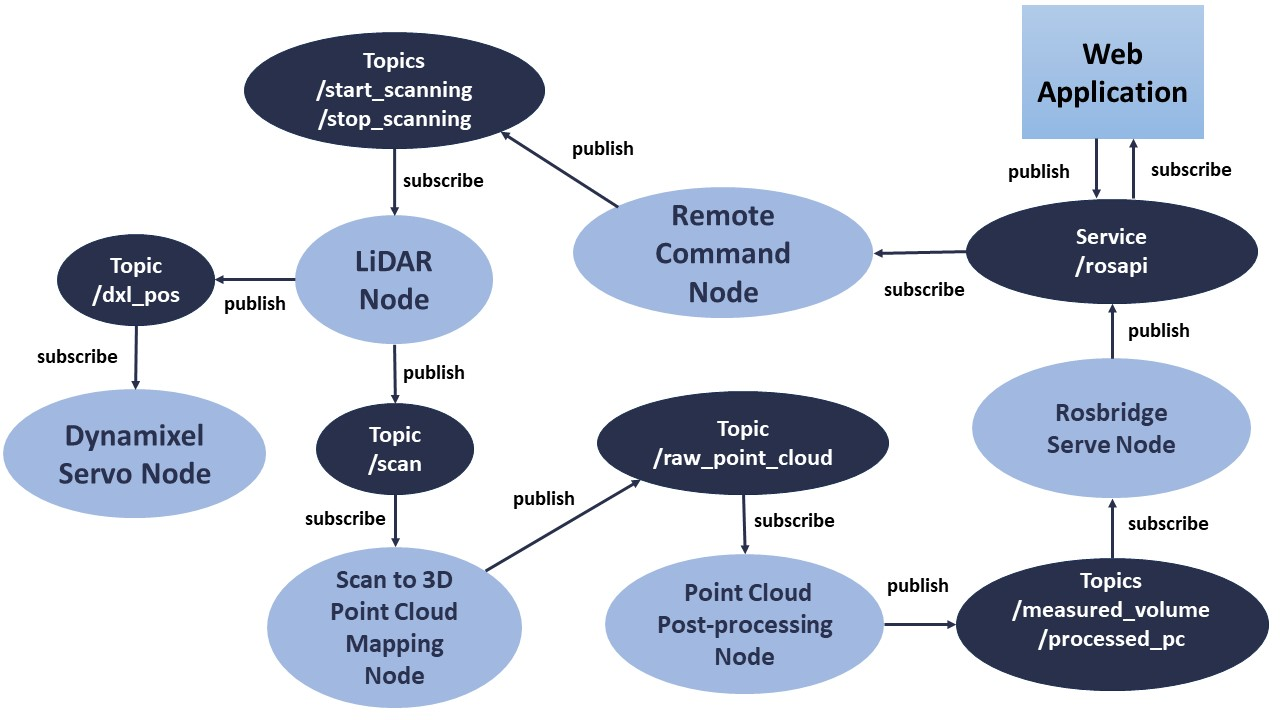
\includegraphics[width=1\textwidth]{Figures/nodes-topics-relationship}
	\caption{Nodes, Topics and their Relationships}
	\label{ch4:fig:nodes-topics-relationships}
\end{figure}

\section{Web-based User Interface Implementation}
A variety set of tools and frameworks were employed to enhance the functionality of the Web Interface. Table \ref{ch3:tab:tools-frameworks} outlines the various tools, frameworks, and libraries utilized in the implementation of the web-based user interface.

\begin{table}[H]
	\centering
	\caption{Tools and Frameworks Used in the Web-based User Interface}
	\label{ch3:tab:tools-frameworks}
	\begin{tabular}{|l|p{9cm}|}
		\hline
		\textbf{Tool/Framework} & \textbf{Description/Functionality}                                                                                                                                                \\ \hline
		jQuery                  & Used for simplifying JavaScript programming and DOM manipulation, jQuery is included via CDN for easy integration.                                                                \\ \hline
		Three.js                & This JavaScript library is utilized for rendering 3D graphics in a web browser. It enables the display of the 3D point cloud viewer within the application.                       \\ \hline
		EventEmitter2           & EventEmitter2 is employed for implementing event-driven programming, allowing efficient communication between different components of the application.                            \\ \hline
		roslib.js               & roslib.js is utilized for connecting the web application to the Robot Operating System (ROS), enabling communication with ROS nodes and topics.                                   \\ \hline
		Bootstrap               & The Bootstrap framework is employed for responsive design and styling of the user interface components. It ensures consistency and enhances the visual appeal of the application. \\ \hline
		Chart.js                & This JavaScript library is used for creating interactive charts and graphs to visualize data. It enhances the user experience by providing intuitive data representation.         \\ \hline
		ros3d.js                & ros3d.js is utilized for integrating ROS visualization capabilities into the web application. It facilitates the display of ROS topics such as point clouds and robot models.     \\ \hline
	\end{tabular}
\end{table}


These tools and frameworks collectively contribute to the functionality of the web-based user interface for the 3D-PCSS.

\subsection{UI Different Dashboard}
\subsubsection*{Main Dashboard Section}
The main dashboard of the UI, as shown in Figure X, consists of three distinct sections. On the left side, the System Status section provides visual feedback regarding the establishment of the connection with the system, allowing users to monitor and verify the connection status. Additionally, users can access a list of currently active topics by clicking the List of Topics button. In the center section, users can visualize and interact with the 3D point cloud data. This includes functionalities such as zooming in and out, moving the visualization, and conducting analysis. Moreover, in this section the start and stop scanning button is located, enabling users to control the scanning process directly from the dashboard. Finally, on the right side, users can find volume measurement values and other pertinent information, such as storage capacity values. The save button is also located in this section to store the empty space volume, Product volume and the percentage capacity of the storage bin in the database

\begin{figure}[H]
	\centering
	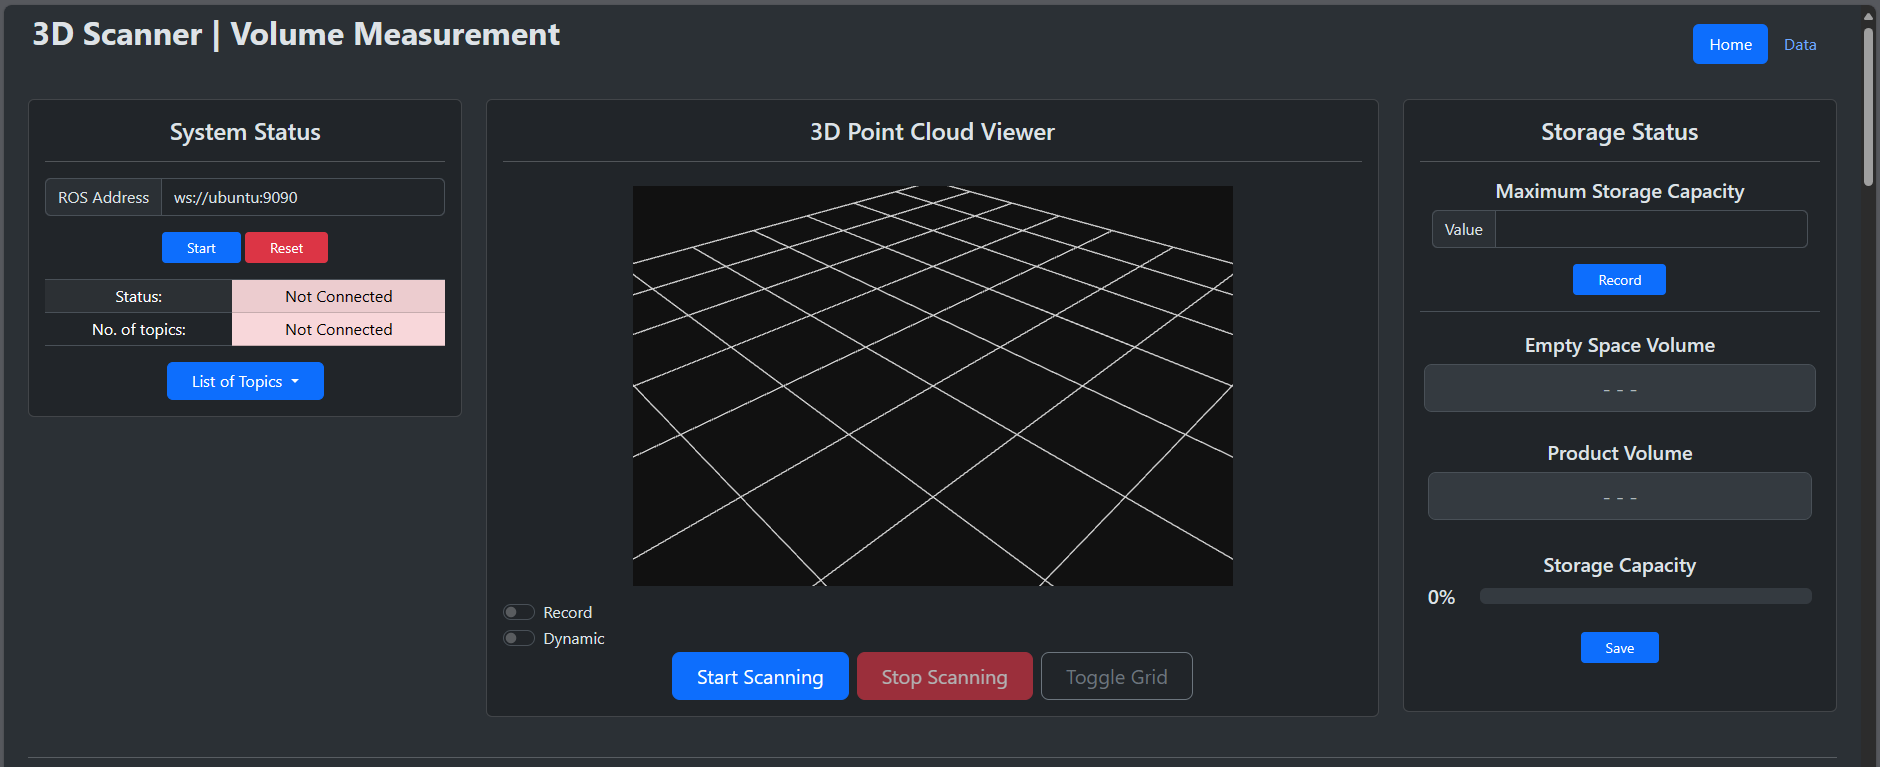
\includegraphics[width=0.9\textwidth]{Figures/main-dashboard}
	\caption{Main Dashboard of Web Interface}
	\label{ch4:fig:main-dashboard}
\end{figure}

\subsubsection*{Data Section}

In the data section of the dashboard, users can visualize both the data table and the graph, as depicted in Figures X and Y, respectively.

\begin{figure}[H]
	\centering
	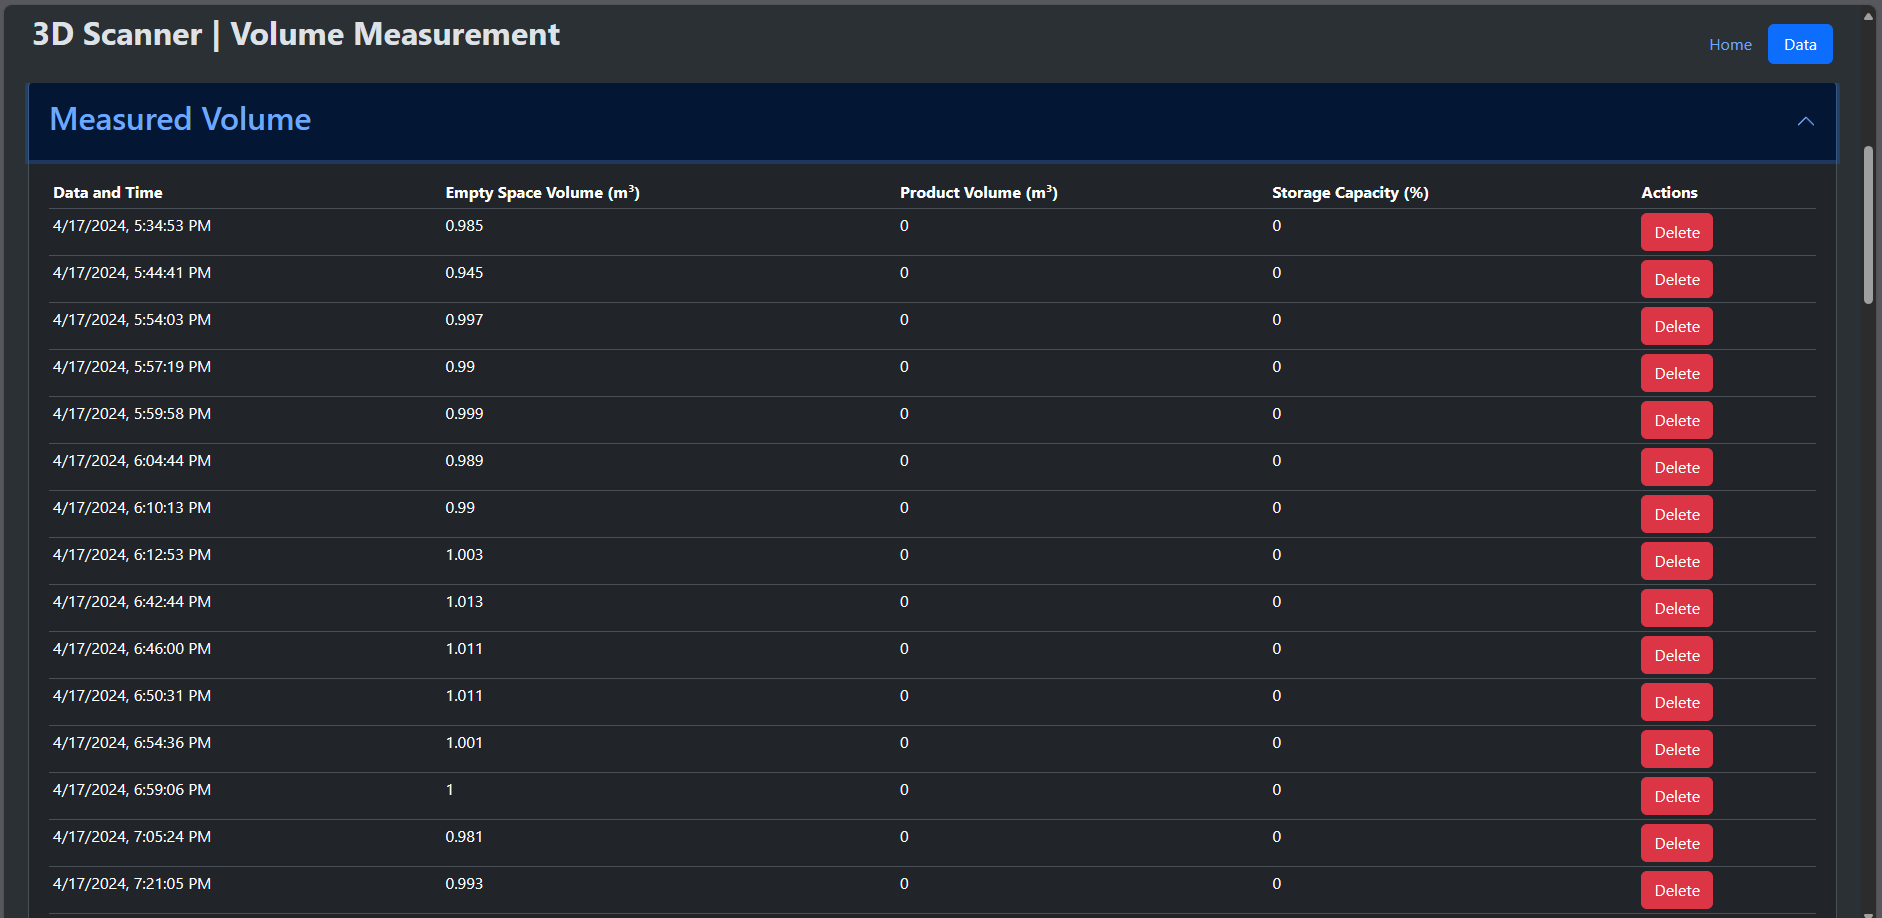
\includegraphics[width=0.9\textwidth]{Figures/main-dashboard-1}
	\caption{Data Dashboard Section Table}
	\label{ch4:fig:main-dashboard-1}
\end{figure}

\begin{figure}[H]
	\centering
	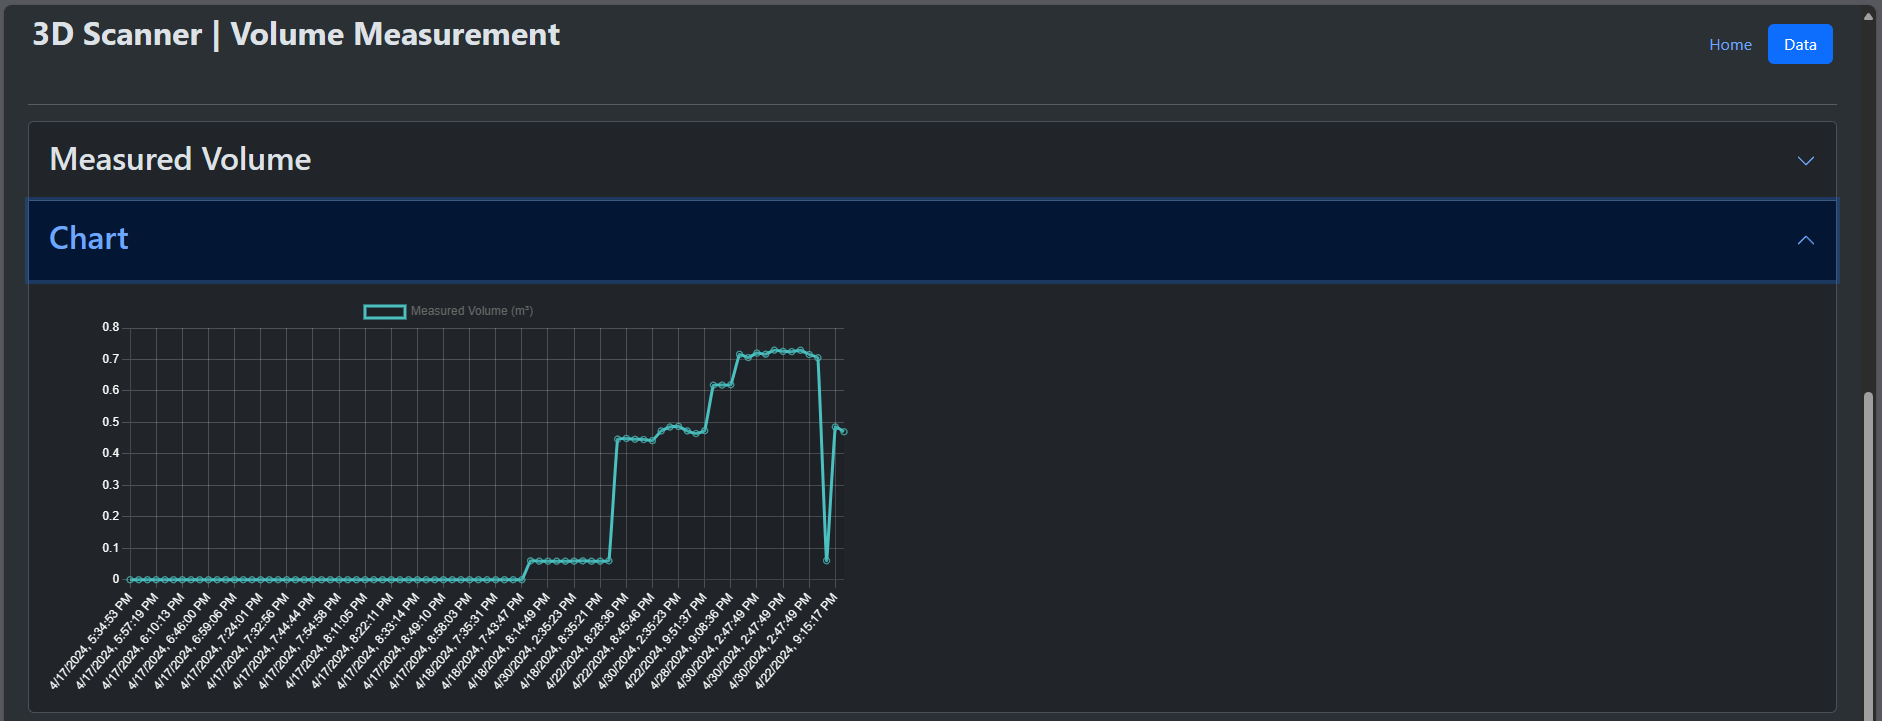
\includegraphics[width=0.9\textwidth]{Figures/main-dashboard-2}
	\caption{Data Dashboard Section Graph}
	\label{ch4:fig:main-dashboard-2}
\end{figure}

\section{Overall System Integration}
The 3D-PCSS and the Web interface were integrated and test their functionalities. This integration includes verifying the connection between the system and the web interface. After verifying the connection between the systems, further tests were conducted to ensure successfully interaction and functionality between the two components. This integration process aimed to validate the overall system's capability to communicate effectively,perform intended tasks such as send and receive command, and visualizing data.


\section{Testing Result and Data Analysis}

After conducting the various tests outlined in Section \ref{ch3:sec:TestingAndEvaluation}, the performance and accuracy of the overall system were evaluated. This section presents the results of each test case along with analysis of the data collected.

\subsection{Created Mock-up Storage Bin}
The design specifications outlined of the proposed storage bin in section \ref{ch3:subsec:constructing-of-storage-bin} were implemented to construct a mock-up storage bin. In the actual mock-up bin consists of three distinct geometric shapes as depicted in Figure \ref{ch4:fig:constructed-storage-bin}. The dimensions of each shape were manually measured using a steel tape measure.

The rectangular shape of the bin measures 2.775 meters in height, with lengths and widths of 0.5 and 0.69 meters respectively. The pyramidal frustum shape has an upper length and width of 0.5 and 0.69 meters respectively, with a height of 0.03 meters, and a lower length and width of 0.42 meters. Lastly, the conical frustum shape features a top radius of 0.21 meters, a bottom radius of 0.17 meters, and a height of 0.42 meters.

With these dimensions, the individual and total volume capacities of the storage bin were calculated. Table \ref{ch4:tab:volume-calculation} provides a summary of the measured individual and total volume capacity of the bin. \\


\begin{table}[H]
	\centering
	\caption{Individual and Total Volume of the Storage Bin}
	\label{ch4:tab:volume-calculation}
	\begin{tabular}{l r}
		\toprule
		\textbf{Shape}    & \textbf{Actual Volume ($m^{3}$)} \\ \midrule

		Rectangular       & 0.9573                           \\

		Pyramidal Frustum & 0.0077                           \\

		Conical Frustum   & 0.0478088                        \\ \midrule

		Total             & 1.012875                         \\ \bottomrule
	\end{tabular}
\end{table}

\begin{figure}[H]
	\centering
	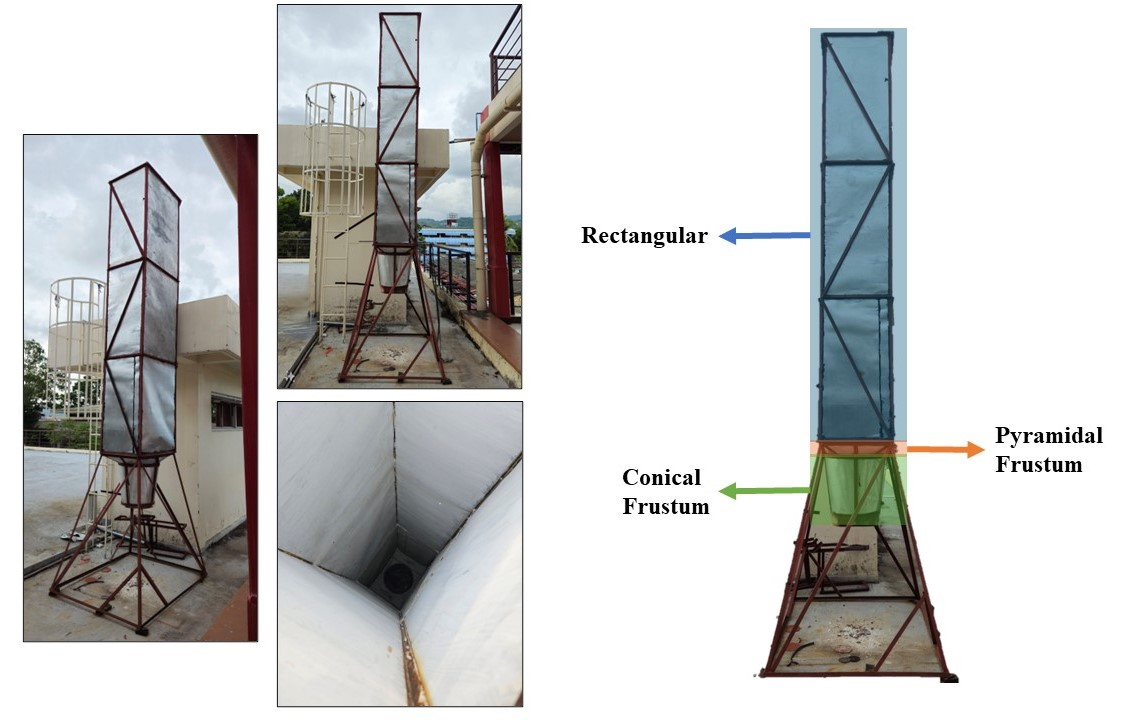
\includegraphics[width=0.9\textwidth]{Figures/constructed_storage_bin.jpg}
	\caption{Constructed Storage Bin Setup}
	\label{ch4:fig:constructed-storage-bin}
\end{figure}

\subsection{Actual System Setup}
The actual field system setup shown in figure \ref{ch4:fig:actual-system-setup} demonstrate the placement of the 3D-PCSS and the laptop where the user interface is running. The actual field of testing situated within the university premises.

\begin{figure}[H]
	\centering
	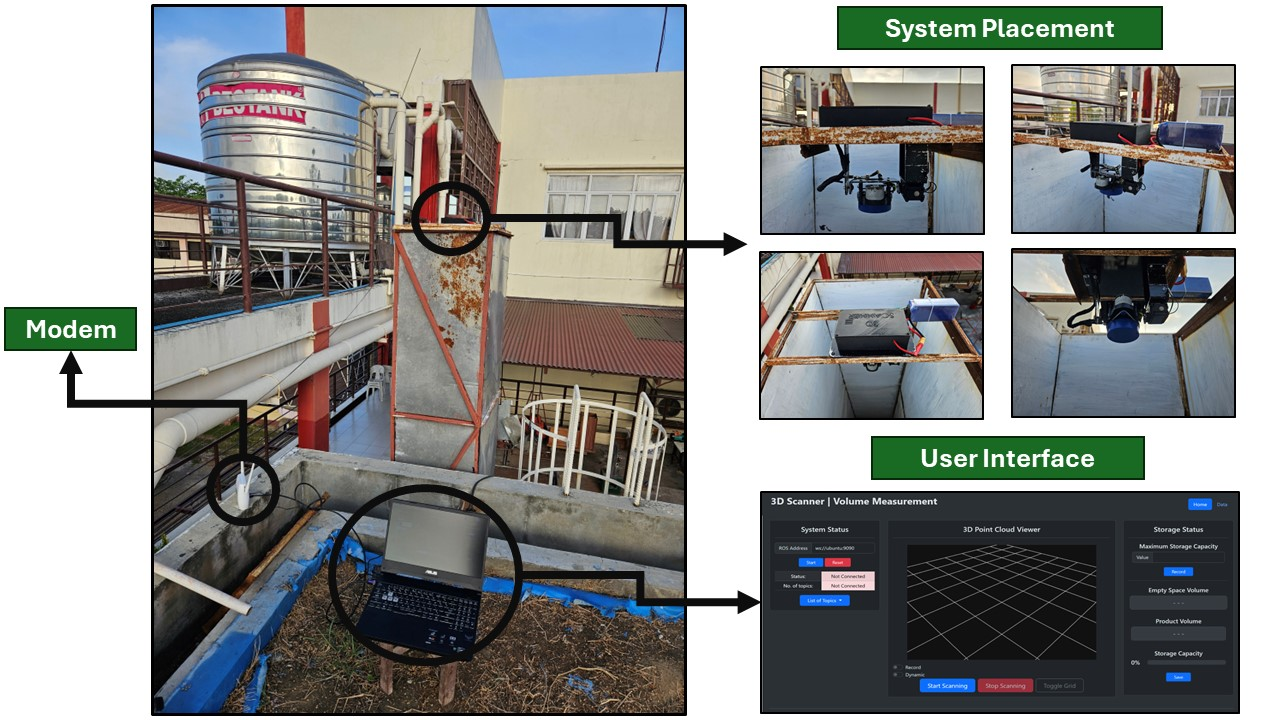
\includegraphics[width=1\textwidth]{Figures/actual-system-setup}
	\caption{Testing Field Actual System Setup}
	\label{ch4:fig:actual-system-setup}
\end{figure}


\subsection{Test Case 1: Empty Storage Bin Scanning}

Multiple scans of an empty storage bin were performed to evaluate the system's performance in accurately measuring the volume of the empty storage bin. Figure \ref{ch4:fig:empty-bin-point-cloud} shows the empty bin with the actual scanned point cloud shape. Table \ref{table:test_case_1_results} summarizes the results obtained from 37 scanning trials.

\begin{figure}[H]
	\centering
	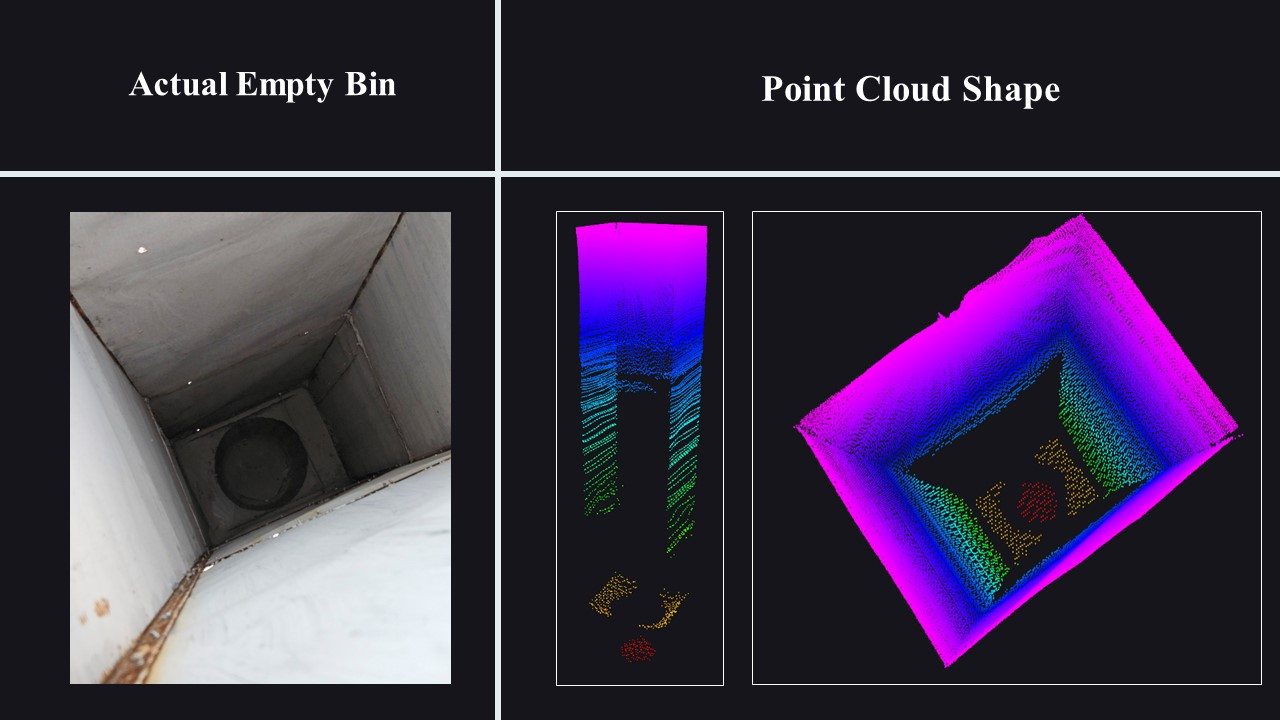
\includegraphics[width=1\textwidth]{Figures/empty-bin-point-cloud}
	\caption{Constructed Storage Bin Setup}
	\label{ch4:fig:empty-bin-point-cloud}
\end{figure}

\begin{table}[H]
	\centering
	\caption{Results of Test Case 1: Empty Storage Bin Scanning}
	\label{table:test_case_1_results}
	\begin{tabular}{l c r}
		\toprule
		\textbf{Trials} & \textbf{Actual Volume ($m^{3}$)} & \textbf{Measured Volume} ($m^{3}$) \\ \midrule

		1               & 1.012875                         & 0.997                              \\
		2               & 1.012875                         & 0.99                               \\
		3               & 1.012875                         & 0.999                              \\
		4               & 1.012875                         & 0.99                               \\
		5               & 1.012875                         & 1.003                              \\
		6               & 1.012875                         & 1.013                              \\
		7               & 1.012875                         & 1.011                              \\
		8               & 1.012875                         & 1.011                              \\
		9               & 1.012875                         & 1.001                              \\
		10              & 1.012875                         & 1                                  \\
		11              & 1.012875                         & 0.993                              \\
		12              & 1.012875                         & 1.007                              \\
		13              & 1.012875                         & 1.011                              \\
		14              & 1.012875                         & 1.019                              \\
		15              & 1.012875                         & 1.021                              \\
		16              & 1.012875                         & 1.013                              \\
		17              & 1.012875                         & 1.014                              \\
		18              & 1.012875                         & 1.006                              \\
		19              & 1.012875                         & 1.003                              \\
		20              & 1.012875                         & 1.01                               \\
		21              & 1.012875                         & 1.013                              \\
		22              & 1.012875                         & 1.016                              \\
		23              & 1.012875                         & 1.014                              \\
		24              & 1.012875                         & 1.014                              \\
		25              & 1.012875                         & 1.016                              \\
		26              & 1.012875                         & 1.015                              \\
		27              & 1.012875                         & 1.011                              \\
		28              & 1.012875                         & 1.011                              \\
		29              & 1.012875                         & 1.007                              \\
		30              & 1.012875                         & 1.016                              \\
		31              & 1.012875                         & 1.017                              \\
		32              & 1.012875                         & 1.009                              \\
		33              & 1.012875                         & 1.007                              \\
		34              & 1.012875                         & 1.017                              \\
		35              & 1.012875                         & 1.017                              \\
		36              & 1.012875                         & 1.014                              \\
		37              & 1.012875                         & 1.014                              \\ \bottomrule
	\end{tabular}
\end{table}

\begin{figure}[H]
	\centering
	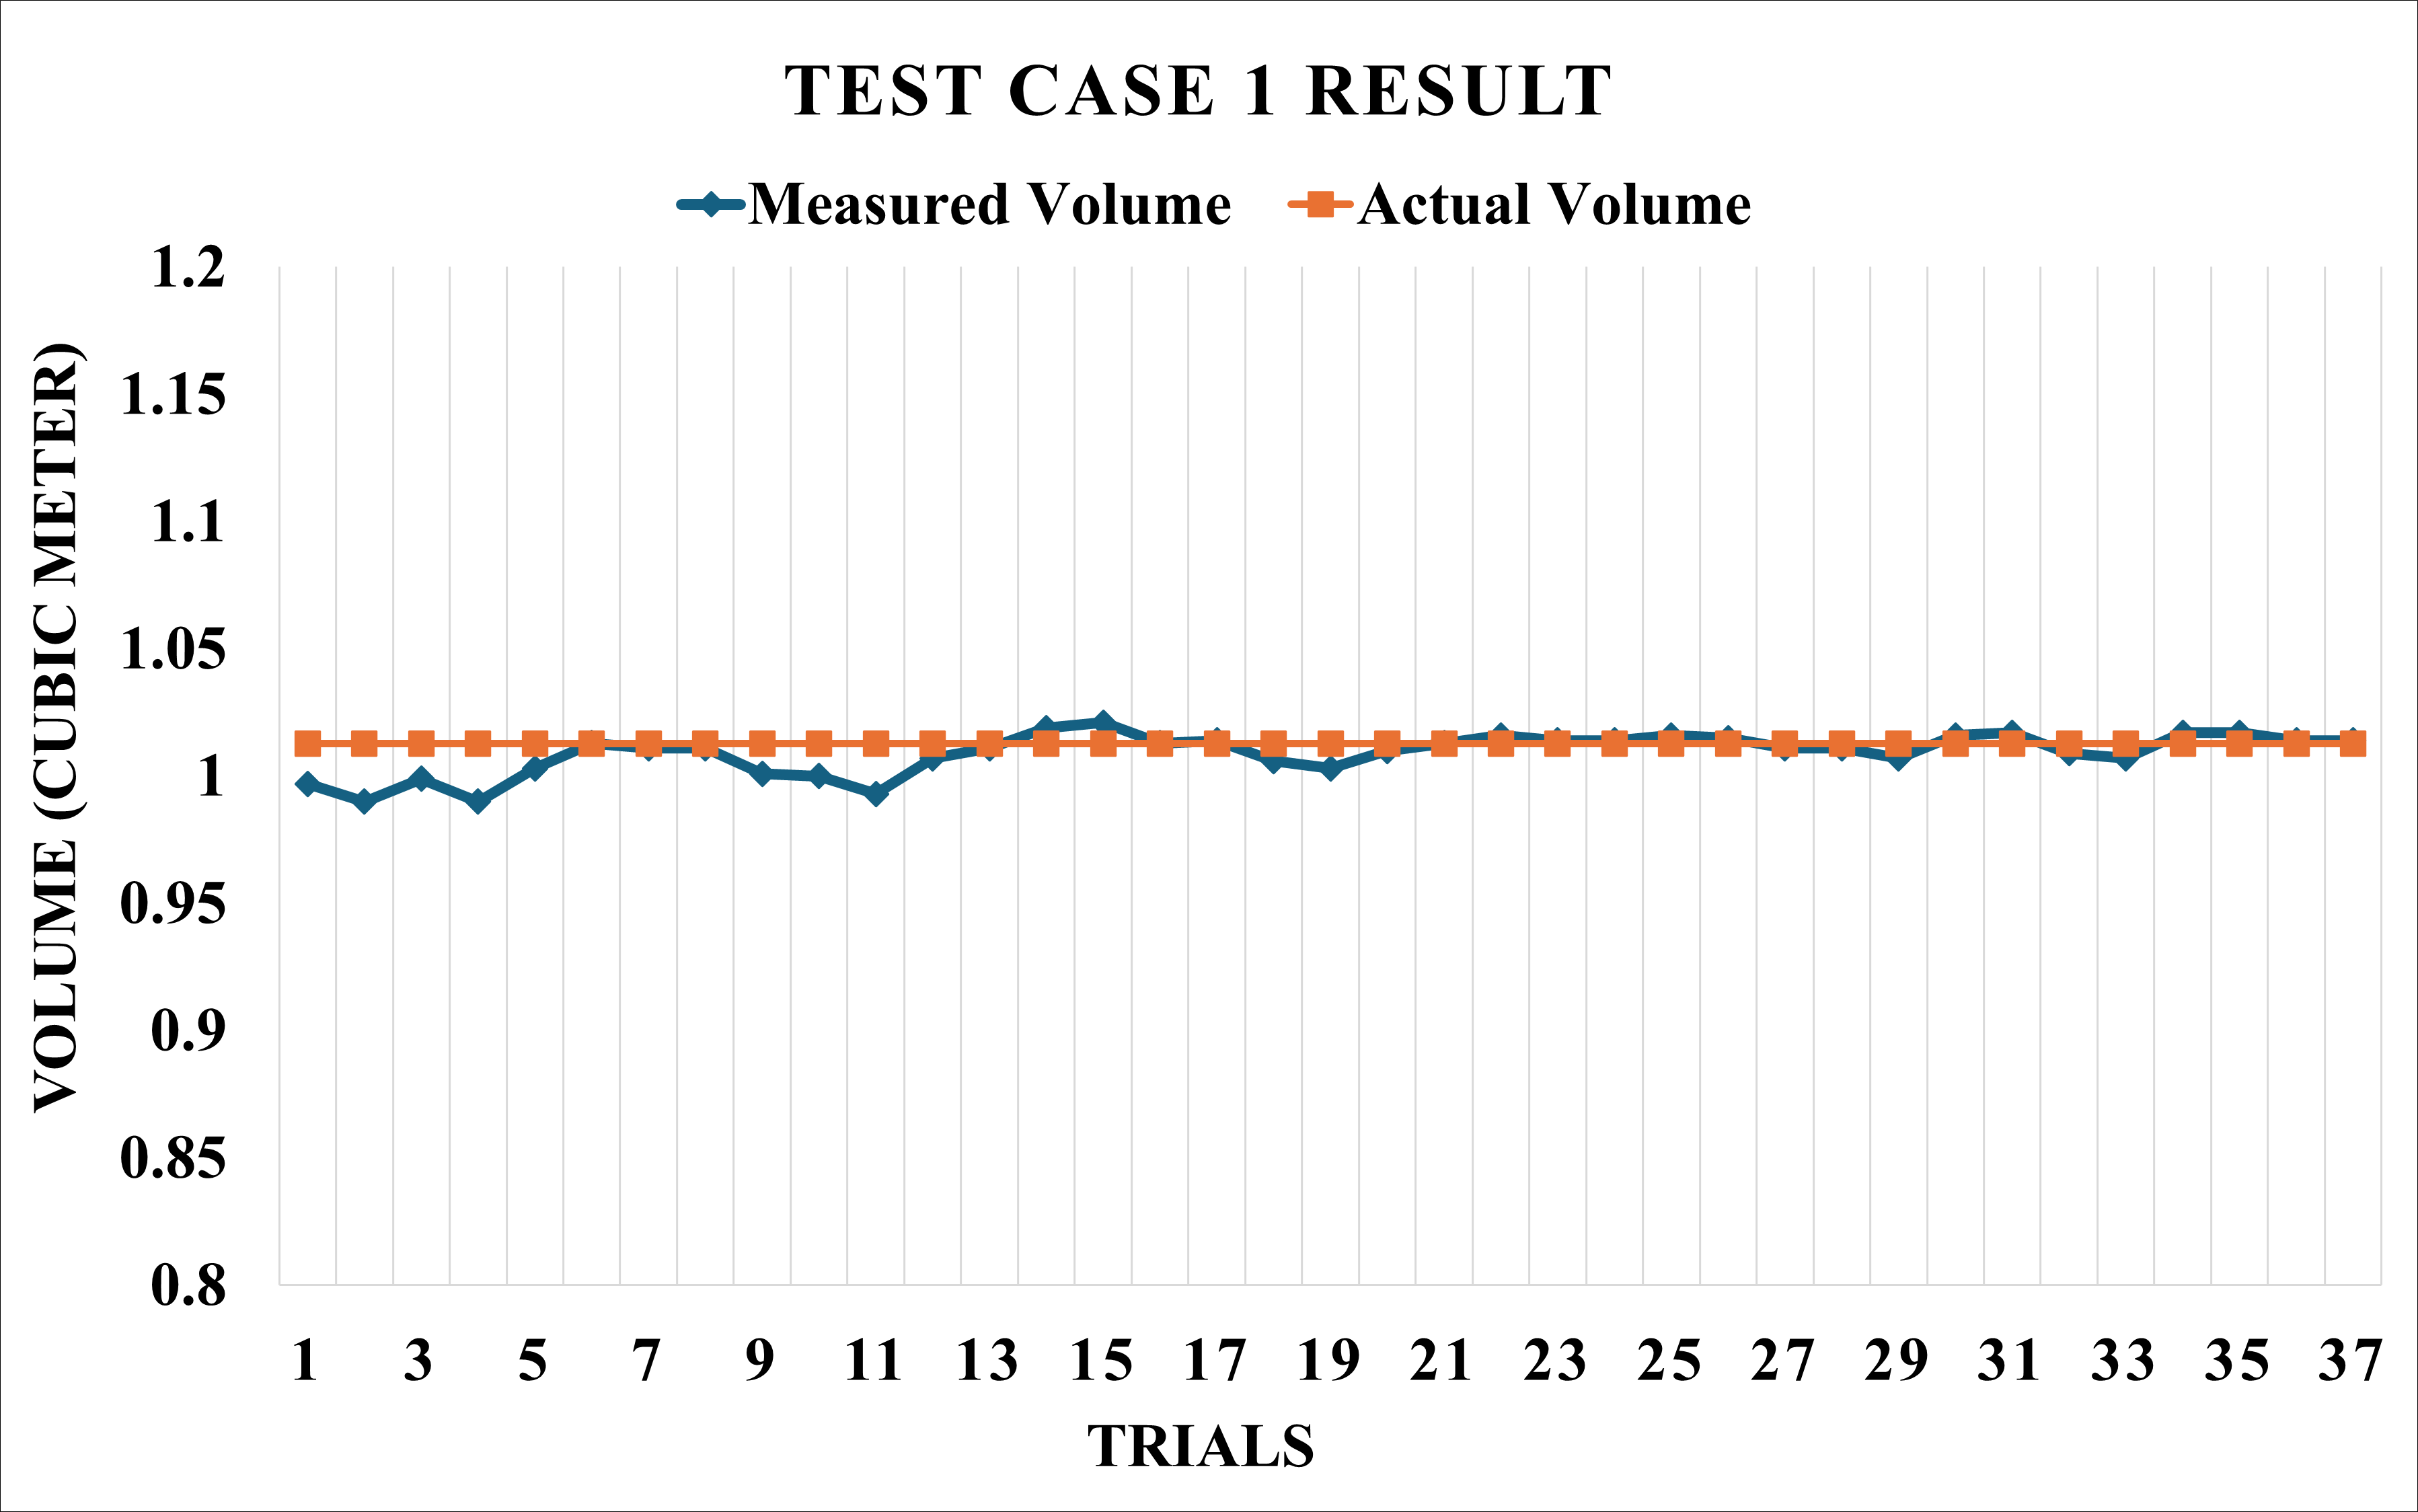
\includegraphics[width=0.8\textwidth]{Figures/test-case-1-graph}
	\caption{Distribution of the Measured Volume with 37 Trials on Test Case 1}
	\label{ch4:fig:test-case-1-graph}
\end{figure}

The average measured volume across all trials was determined to be 1.00919 $\pm$ 0.00784 $m^{3}$, indicating a standard deviation of 0.00784 $m^{3}$. With a gathered Mean Absolute Percentage Error (MAPE) of 0.599377608 \%. This average volume of the empty storage bin was subsequently used as the maximum volume capacity for the next testing cases. The distribution of the data gathered can be visualize in the figure \ref{ch4:fig:test-case-1-graph}

\subsection{Test Case 2: Filling the Storage Bin with Known Volume}

In this test case, three different scenarios were conducted to evaluate the system's accuracy in measuring the volume of flour filled into the storage bin with different storage percentage capacity such as: 5.8\%, 47.2\% and 70.3\% of the storage's maximum capacity, the storage bin was filled with a known volume using the container shown in figure \ref{ch4:fig:known-volume}. Each scenario conducted two different flour surface contour as outline in section \ref{ch3:subsec:test-case-2}. The results show the different flour surface contour first, followed by the data table.

\begin{figure}[H]
	\centering
	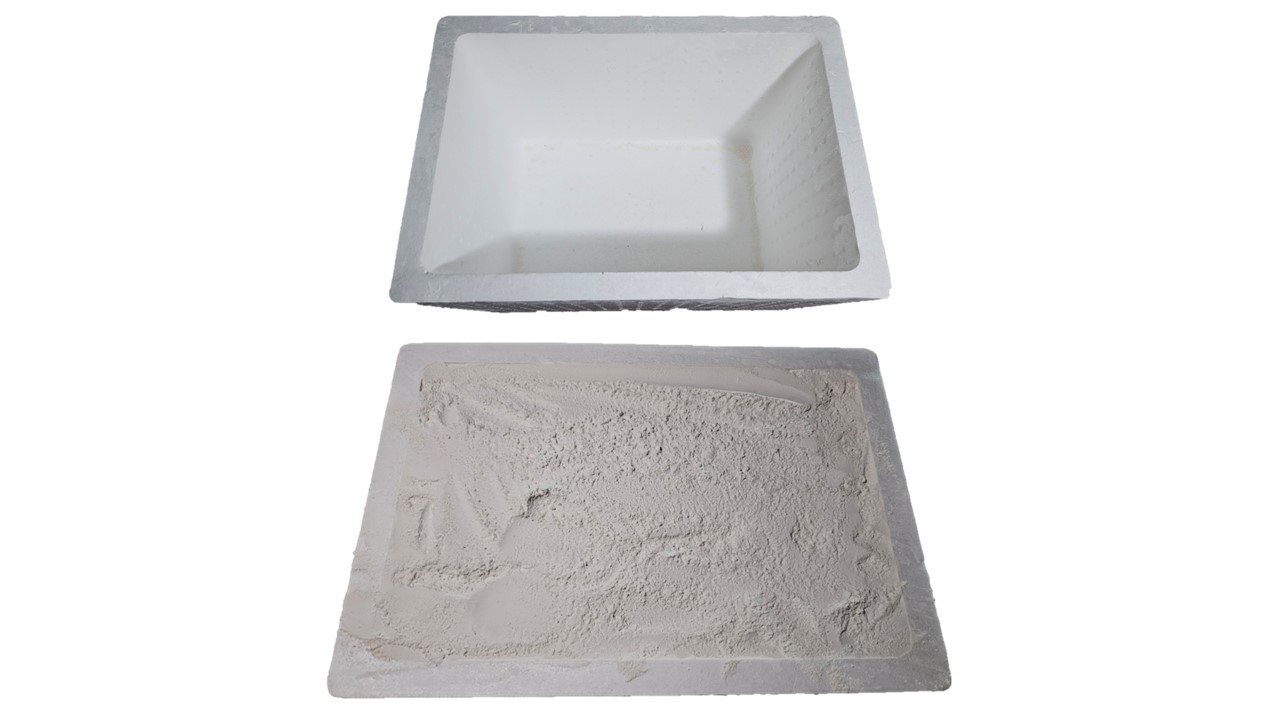
\includegraphics[width=0.8\textwidth]{Figures/known-volume}
	\caption{Container with a Known Volume Used for Testing}
	\label{ch4:fig:known-volume}
\end{figure}


\subsubsection*{Test Case 2.1: Storage Bin Filled to 5.8\% of Maximum Capacity}

\begin{figure}[H]
	\centering
	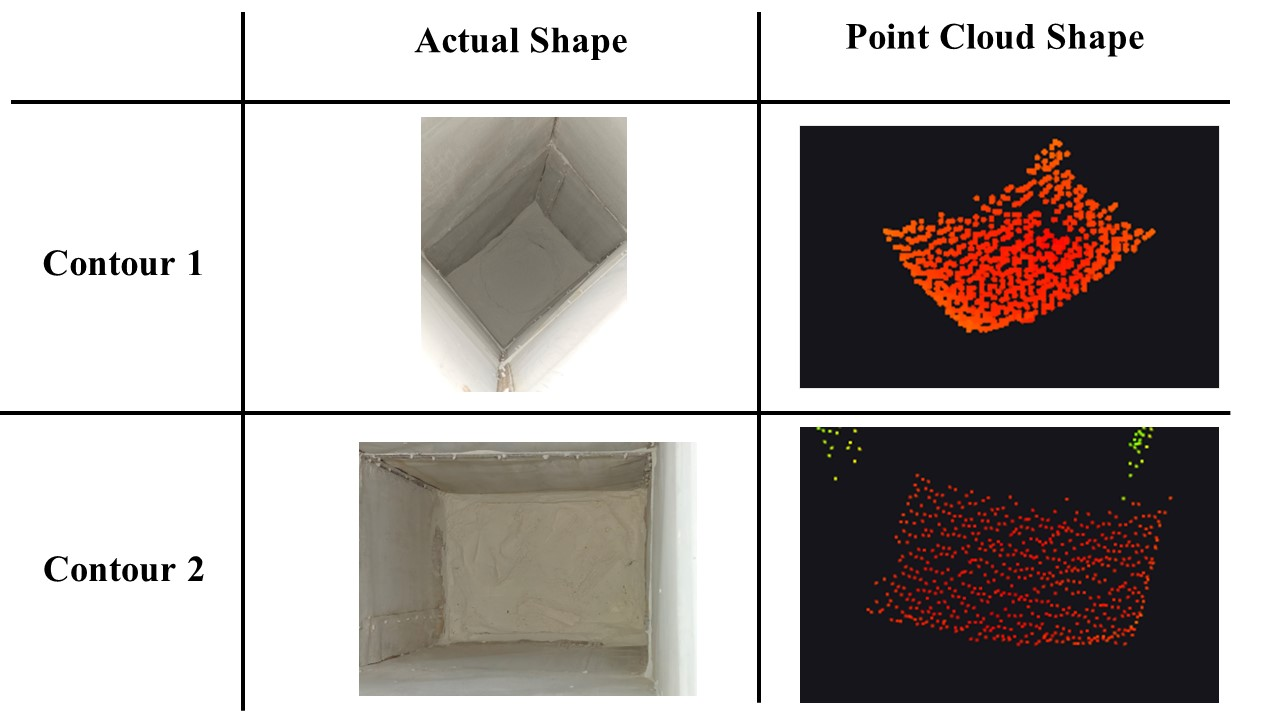
\includegraphics[width=0.8\textwidth]{Figures/test_2-1_contours}
	\caption{Different Flour Surface Contour of Test 2.1}
	\label{ch4:fig:test_2-1_contours}
\end{figure}

\begin{table}[H]
	\centering
	\caption{Test Case 2.1 Result}
	\label{table:test_case_2-1_results}
	\begin{tabular}{l c c r}
		\toprule
		\textbf{Trials} & \multicolumn{2}{c}{\textbf{Measured Volume ($m^{3}$)}} & \textbf{Actual Volume} ($m^{3}$)          \\
		{}              & Contour 1                                              & Contour 2                        & {}     \\ \midrule
		1               & 0.06                                                   & 0.0592                           & 0.0594 \\
		2               & 0.05934                                                & 0.0601                           & 0.0594 \\
		3               & 0.058943                                               & 0.0589                           & 0.0594 \\
		4               & 0.05976                                                & 0.0591                           & 0.0594 \\
		5               & 0.059678                                               & 0.0602                           & 0.0594 \\ \midrule
		Average         & 0.059678                                               & 0.0595                           & {}     \\ \bottomrule
	\end{tabular}
\end{table}

\begin{figure}[H]
	\centering
	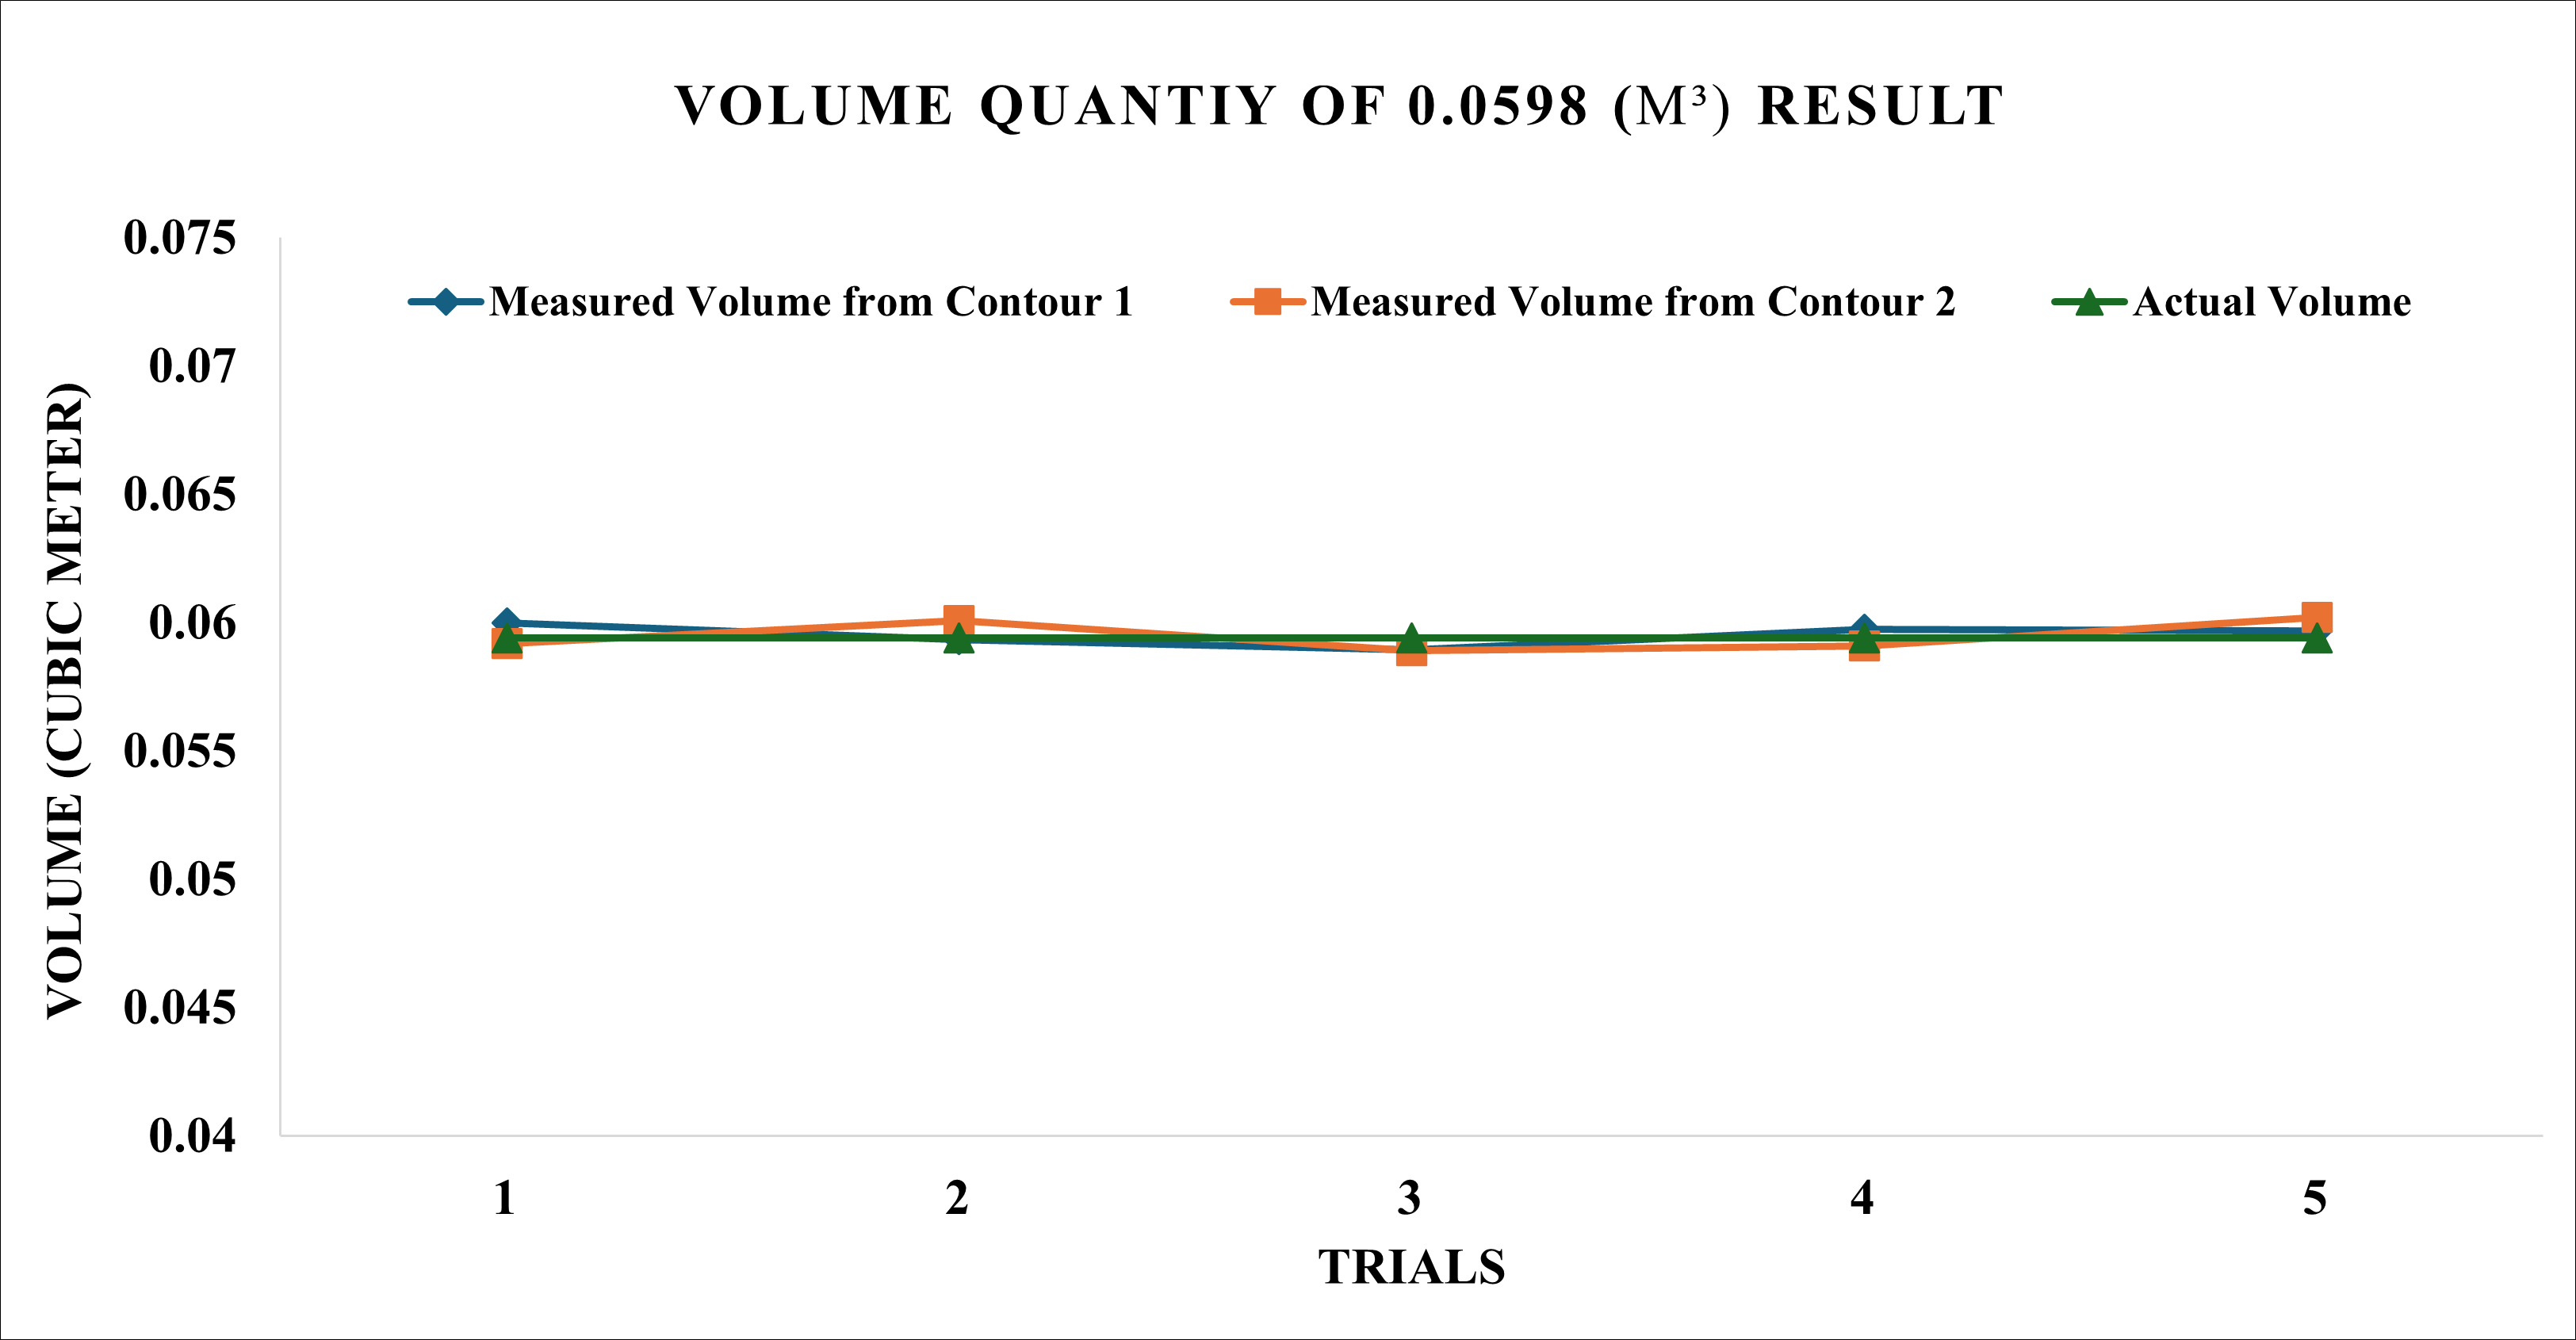
\includegraphics[width=0.8\textwidth]{Figures/test-case-2-1-graph}
	\caption{Distribution of the Measured Volume on Test Case 2.1}
	\label{ch4:fig:test-case-2-1-graph}
\end{figure}



The results from Test Case 2.1 gathered an average measured volume of 0.059678 $m^{3}$ and 0.0595 $m^{3}$ and a deviation of 0.00036 $m^{3}$ and 0.00054 $m^{3}$ from contour 1 and 2 respectively. Contour 1 achieved a MAPE of 0.591\%, while the contour 2 have a MAPE of 0.8417\%. Overall, Test Case 2.1 gathered an average measured volume with standard deviation of 0.0595221 $\pm$ 0.0004626 $m^{3}$ and a MAPE of 0.7163\%.

%\subsection{Discussion}

%%%The test results demonstrate the effectiveness and accuracy of the developed 3D-PCSS in measuring the volume of both empty and filled storage bins. The system consistently provided reliable measurements across multiple trials and scenarios, validating its suitability for practical applications in various industries. Further analysis of the data collected revealed minor discrepancies between the measured and actual volumes, which can be attributed to factors such as sensor calibration and environmental conditions. Overall, the system performed satisfactorily and met the objectives set forth in this study. \\

%%%%%%%%%%%%%%%%%%%%%%%%%%%%%%%%%%%%%%%%%%%%%%

\subsubsection*{Test Case 2.2: Storage Bin Filled to 47.2\% of Maximum Capacity}

\begin{figure}[H]
	\centering
	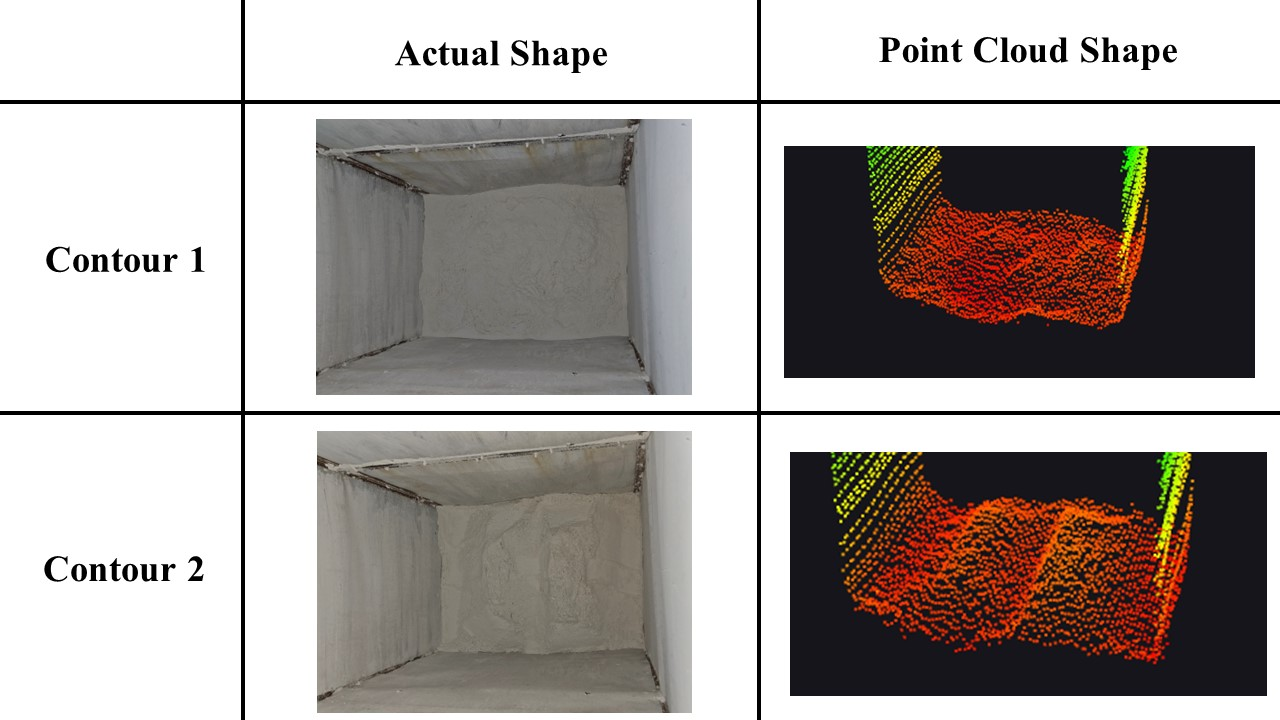
\includegraphics[width=0.8\textwidth]{Figures/test_2-2_contours}
	\caption{Different Flour Surface Contour of Test 2.2}
	\label{ch4:fig:test_2-2_contours}
\end{figure}
\begin{table}[H]
	\centering
	\caption{Test Case 2.2 Result}
	\label{table:test_case_2-2_results}
	\begin{tabular}{l c c r}
		\toprule
		\textbf{Trials} & \multicolumn{2}{c}{\textbf{Measured Volume ($m^{3}$)}} & \textbf{Actual Volume} ($m^{3}$)          \\
		{}              & Contour 1                                              & Contour 2                        & {}     \\ \midrule
		1               & 0.470418                                               & 0.472914                         & 0.4752 \\
		2               & 0.470279                                               & 0.464461                         & 0.4752 \\
		3               & 0.472061                                               & 0.473782                         & 0.4752 \\
		4               & 0.4805594                                              & 0.485587                         & 0.4752 \\
		5               & 0.4770345                                              & 0.470211                         & 0.4752 \\ \midrule
		Average         & 0.47407038                                             & 0.473391                         & {}     \\ \bottomrule
	\end{tabular}
\end{table}

\begin{figure}[H]
	\centering
	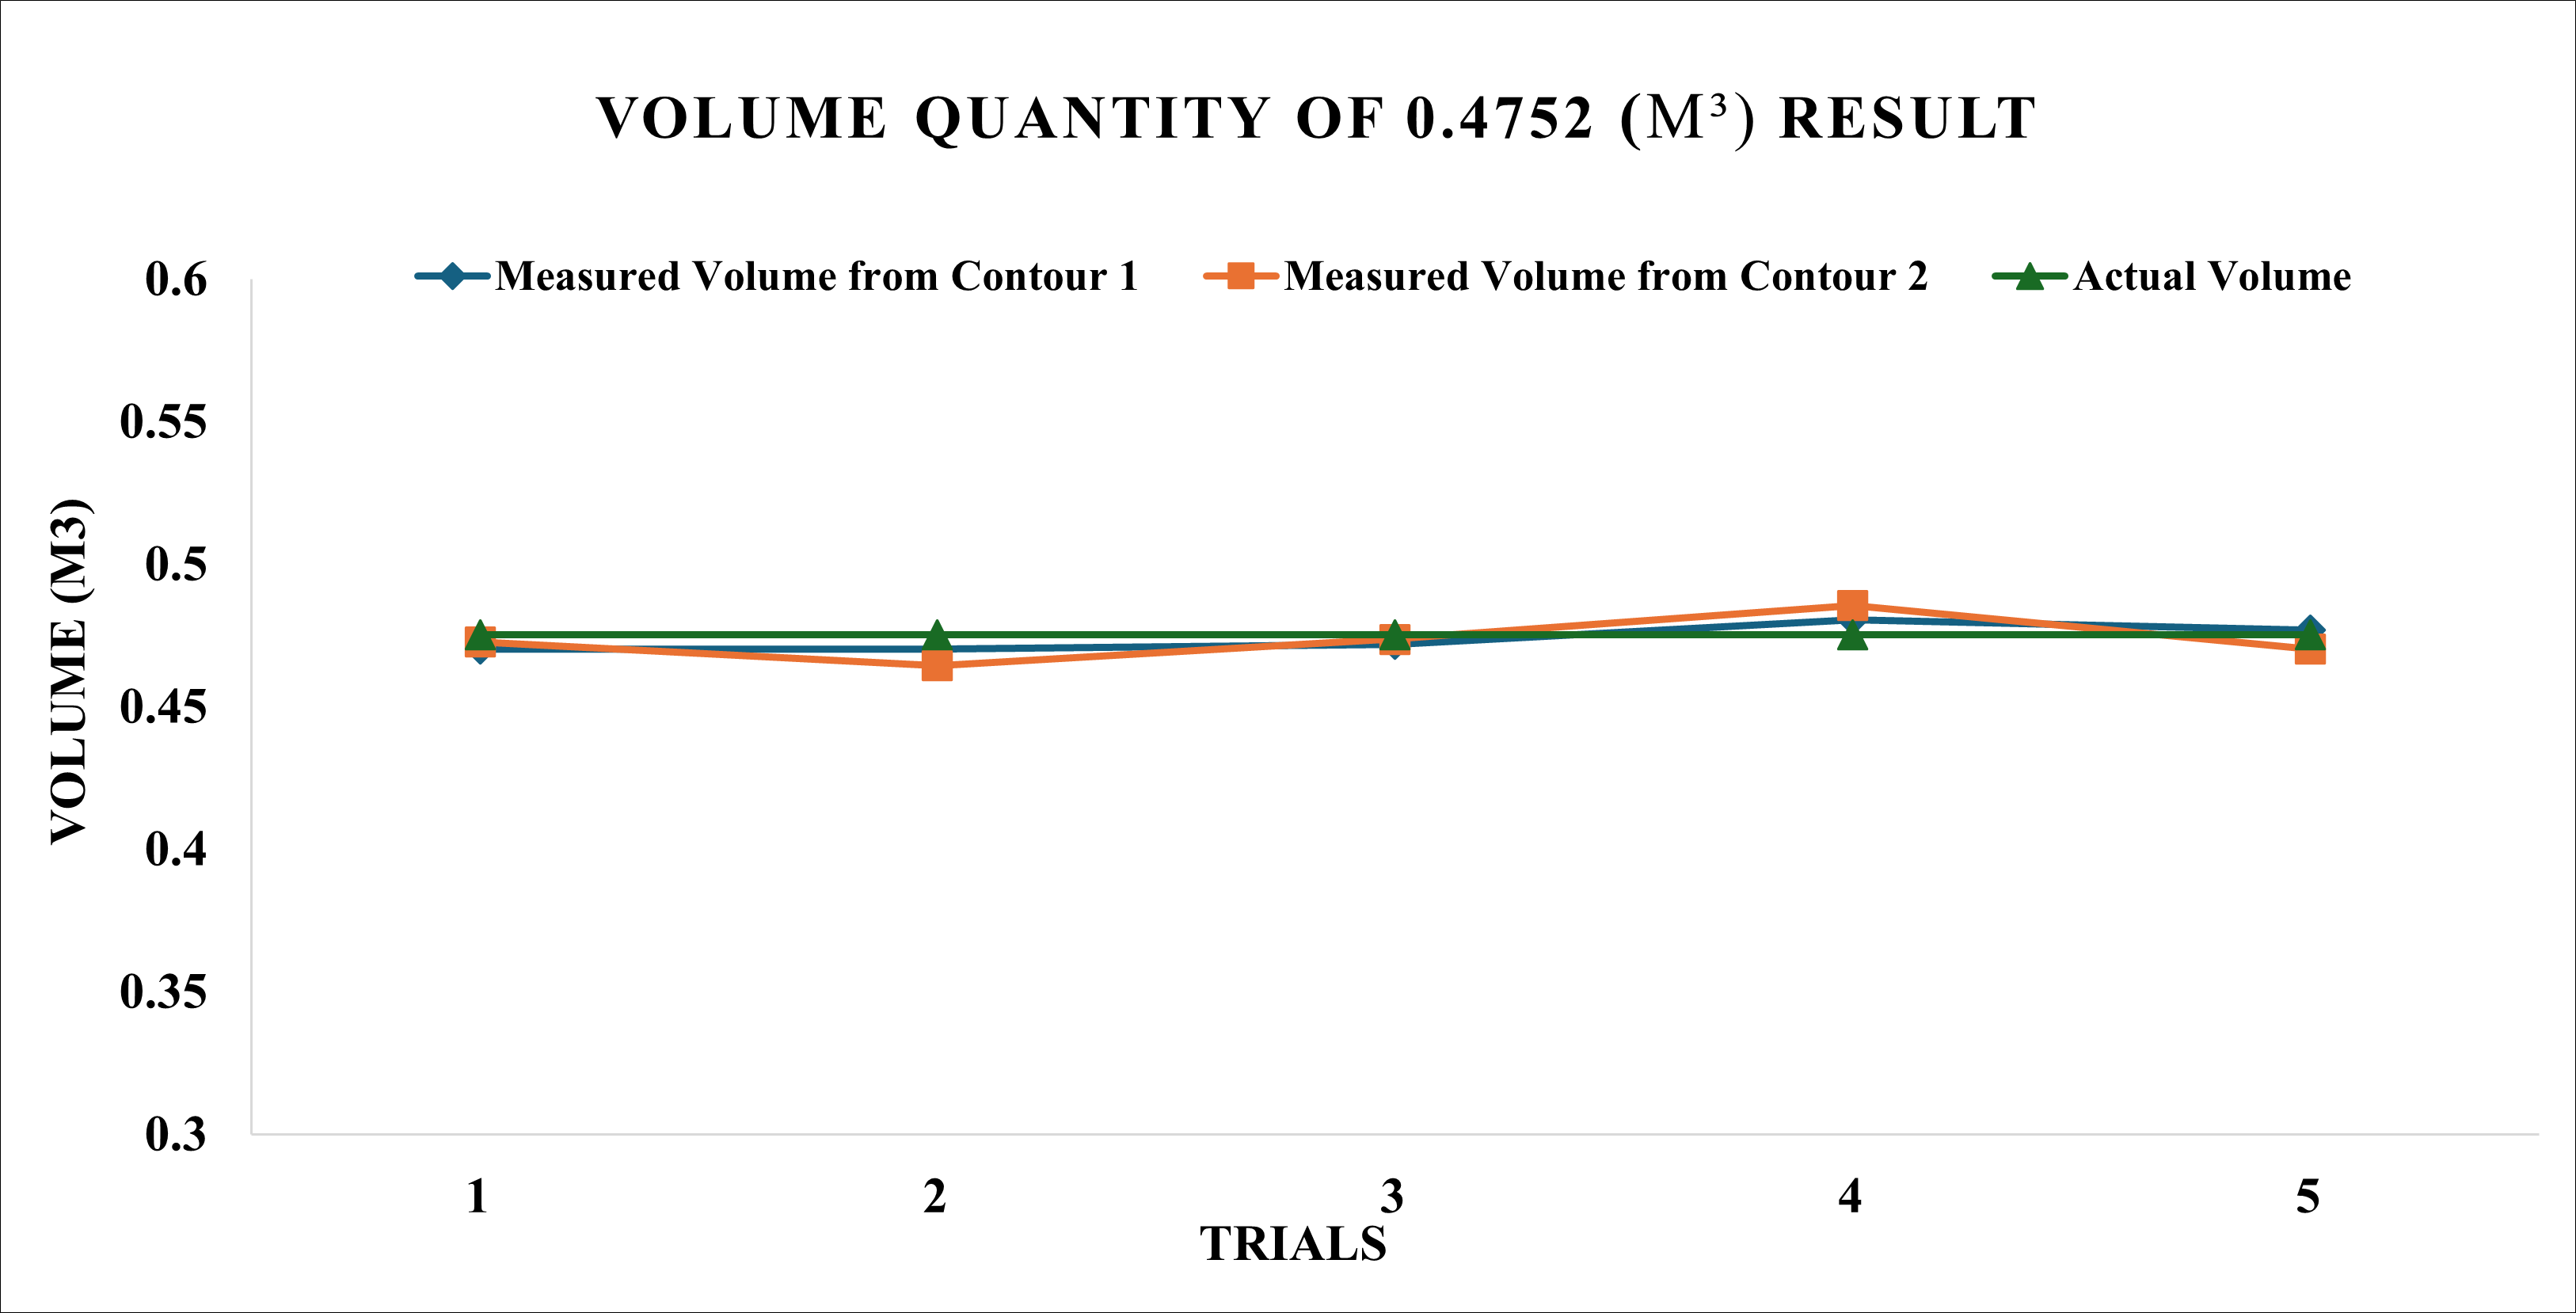
\includegraphics[width=0.8\textwidth]{Figures/test-case-2-2-graph}
	\caption{Distribution of the Measured Volume on Test Case 2.2}
	\label{ch4:fig:test-case-2-2-graph}
\end{figure}

The results from Test Case 2.2 gathered an average measured volume of 0.47407038 $m^{3}$ and 0.4733912158 $m^{3}$ and a deviation of 0.00406 $m^{3}$ and 0.00691 $m^{3}$ from contour 1 and 2 respectively. Contour 1 achieved a MAPE of 0.8432\%, while the contour 2 have a MAPE of 1.2549\%. Overall, Test Case 2.2 gathered an average measured volume with a standard deviation of 0.47373 $\pm$ 0.00568 $m^{3}$ and a MAPE of 1.04912\%.

\subsubsection*{Test Case 2.3: Storage Bin Filled to 70.37\% of Maximum Capacity}
\begin{figure}[H]
	\centering
	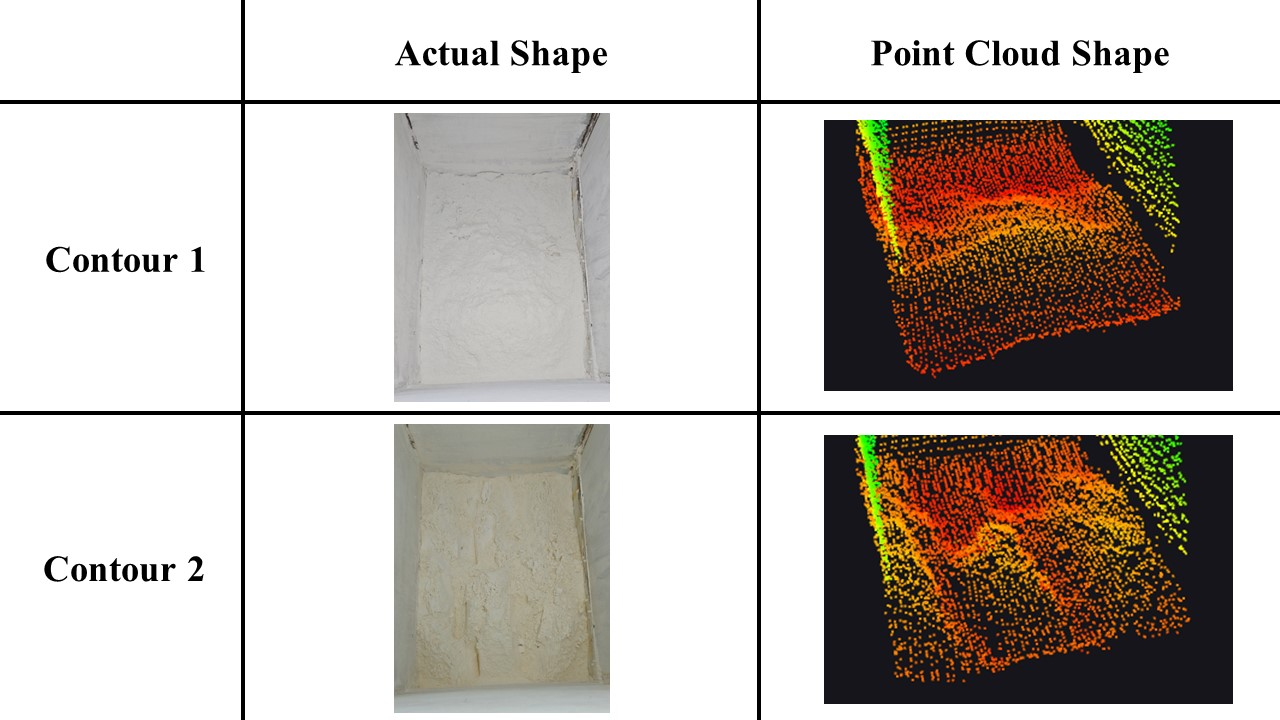
\includegraphics[width=0.8\textwidth]{Figures/test_2-3_contours}
	\caption{Different Flour Surface Contour of Test 2.3}
	\label{ch4:fig:test_2-3_contours}
\end{figure}

\begin{table}[H]
	\centering
	\caption{Test Case 2.3 Result}
	\label{table:test_case_2-3_results}
	\begin{tabular}{l c c r}
		\toprule
		\textbf{Trials} & \multicolumn{2}{c}{\textbf{Measured Volume ($m^{3}$)}} & \textbf{Actual Volume} ($m^{3}$)          \\
		{}              & Contour 1                                              & Contour 2                        & {}     \\ \midrule
		1               & 0.716327                                               & 0.725803                         & 0.7128 \\
		2               & 0.706001                                               & 0.724873                         & 0.7128 \\
		3               & 0.720251                                               & 0.729404                         & 0.7128 \\
		4               & 0.71687                                                & 0.715844                         & 0.7128 \\
		5               & 0.729654                                               & 0.705429                         & 0.7128 \\ \midrule
		Average         & 0.7178206                                              & 0.7202706                        & {}     \\ \bottomrule
	\end{tabular}
\end{table}

\begin{figure}[H]
	\centering
	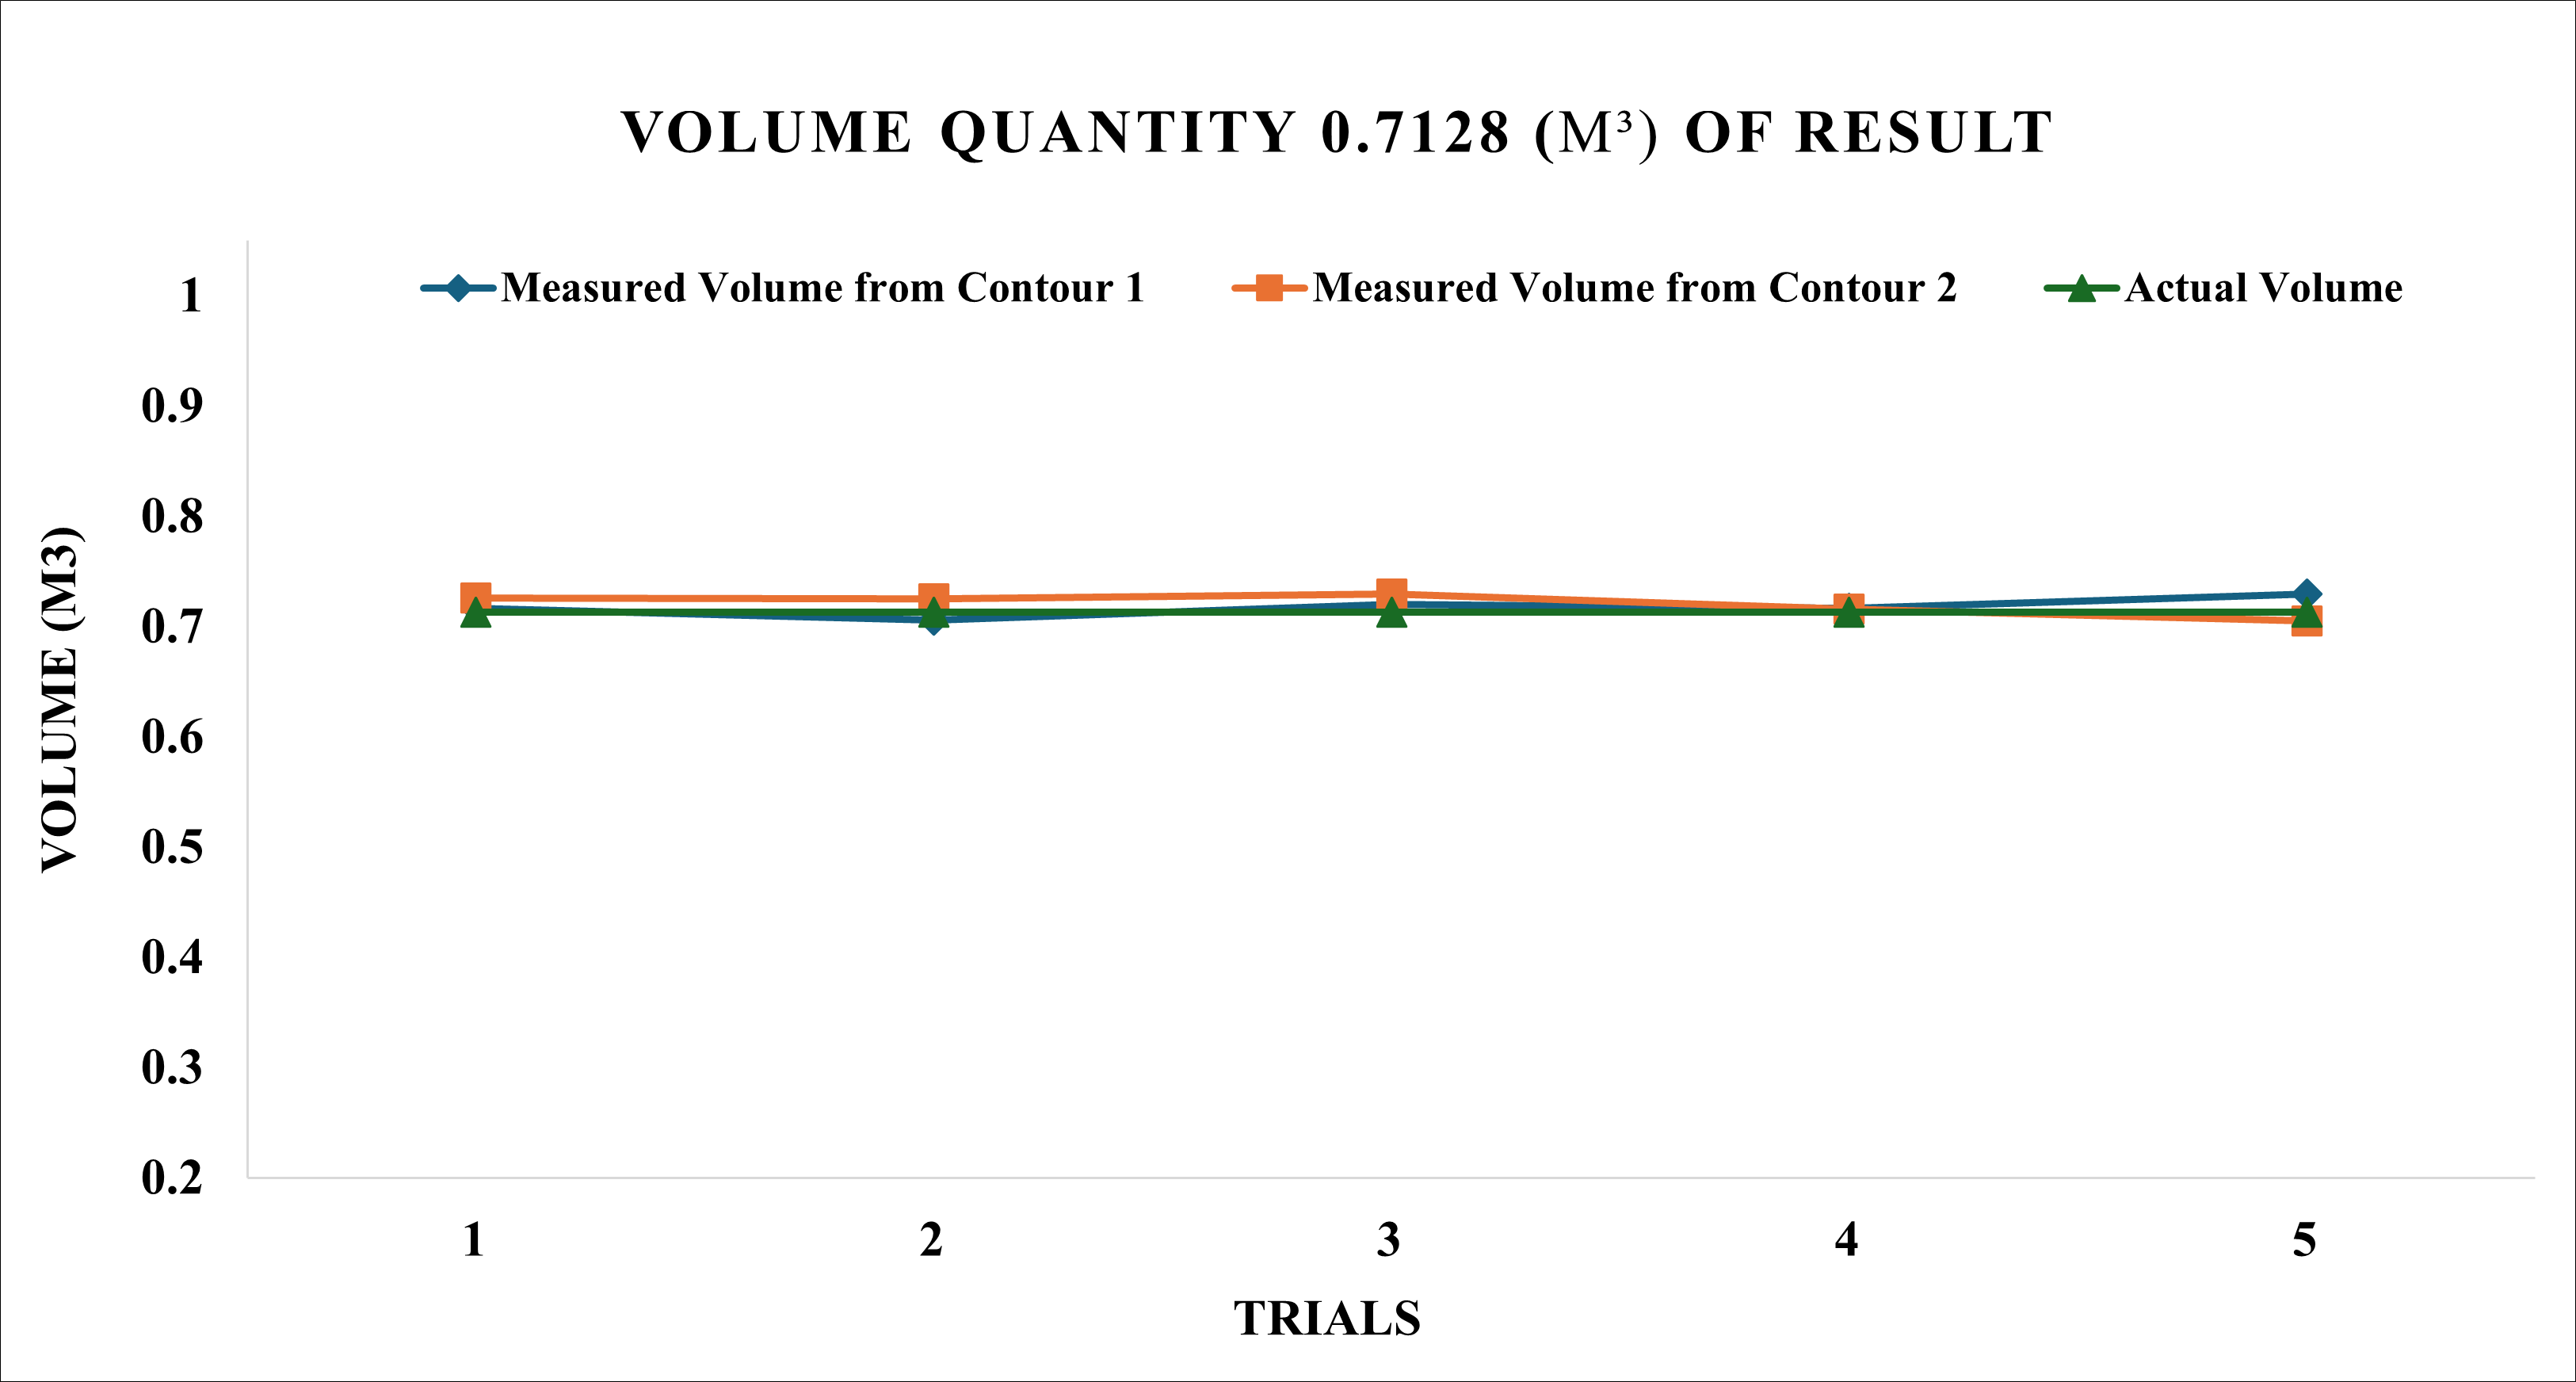
\includegraphics[width=0.8\textwidth]{Figures/test-case-2-3-graph}
	\caption{Distribution of the Measured Volume on Test Case 2.3}
	\label{ch4:fig:test-case-2-3-graph}
\end{figure}


The results from Test Case 2.3 gathered an average measured volume of 0.7178206 $m^{3}$ and 0.7202706 $m^{3}$ and a deviation of 0.0076 $m^{3}$ and 0.0086 $m^{3}$ from contour 1 and 2 respectively. Contour 1 achieved a MAPE of 1.08588\%, while the contour 2 have a MAPE of 1.4617\%. Overall, Test Case 2.3 gathered an average measured volume with a standard deviation of 0.719 $\pm$ 0.008239 $m^{3}$ and a MAPE of 1.27379\%.

\subsubsection*{Summary of Test Case 2 Result}
\begin{table}[H]
	\centering
	\caption{Summary of the of Test Case 2}
	\label{ch4:tab:test-2-summary}
	\begin{tabular}{l c r}
		\toprule
		\textbf{Test} & \textbf{Average Measured Volume with Deviation ($m^{3}$)} & \textbf{MAPE (\%)} \\ \midrule

		2.1           & 0.0595 $\pm$ 0.0004626                                    & 0.71633            \\

		2.2           & 0.47373 $\pm$ 0.00568                                     & 1.04912            \\

		2.3           & 0.719 $\pm$ 0.00824                                       & 1.27379            \\ \midrule

		Average       & {}                                                        & 1.01308            \\ \bottomrule
	\end{tabular}
\end{table}

The table \ref{ch4:tab:test-2-summary} indicates that the system achieved an average MAPE of 1.01308 across the three conducted tests. This suggests that the system is capable of accurately measuring the volume of the flour product across varying storage capacities, up to a maximum level of 70.3\%.

\subsection{Summary of the Conducted Test Cases}

\begin{table}[H]
	\centering
	\caption{Summary of the of Test Case 2}
	\label{ch4:tab:test-cases-summary}
	\begin{tabular}{l l c r}
		\toprule
		\multicolumn{2}{l}{\textbf{Test Cases}} & \textbf{Average Measured Volume with Deviation ($m^{3}$)} & \textbf{MAPE (\%)}                \\ \midrule

		\multicolumn{2}{l}{1}                   & 1.009189 $\pm$ 0.0078356                                  & 0.5993776                         \\

		{}                                      & 2.1                                                       & 0.0595 $\pm$ 0.0004626 & 0.71633  \\

		2                                       & 2.2                                                       & 0.47373 $\pm$ 0.00568  & 1.04912  \\

		{}                                      & 2.3                                                       & 0.719 $\pm$ 0.00824    & 1.27379  \\ \midrule

		Average                                 & {}                                                        & {}                     & 0.909655 \\ \bottomrule
	\end{tabular}
\end{table}

The table \ref{ch4:tab:test-cases-summary} summarizes the two test cases conducted. The system achieved an average MAPE of 0.909655\% indicates an error of $<1\%$ with a highest error of 1.27379\% and lowest error of 0.5993776\%.
\bibliography{References}
\bibliographystyle{apalike}


\end{document}